\documentclass[a4paper,11pt]{report}
\setcounter{errorcontextlines}{999}

%%%pre-amble%%%%%%%%
\usepackage{rotating}
\usepackage{adjustbox}
\usepackage{graphicx}
\usepackage{hyperref} %this makes everything hyper-refed
\usepackage{fancyhdr}
\usepackage{subfigure}
\usepackage{textgreek}
\usepackage{enumitem}
\usepackage{booktabs}
\usepackage{verbatim}
\usepackage{longtable}
\setlength{\LTcapwidth}{9.75in}
\usepackage{multirow}
\usepackage{color}
\usepackage{grffile}
\usepackage{amsmath, amsthm, amssymb}
\usepackage{lscape}
\usepackage[table,xcdraw]{xcolor}
\usepackage{setspace}
\lhead{} 
\usepackage[english]{babel}
\usepackage{csquotes}
\usepackage{float}

\usepackage[
backend=biber,
style=authoryear,
sorting=nyt
]{biblatex}
%\usepackage{biblatex}

\addbibresource{biblio.bib}

 \usepackage{titlesec, blindtext, color}
\definecolor{gray75}{gray}{0.75}
\newcommand{\hsp}{\hspace{1pt}}
\usepackage[a4paper,left=2cm,right=2cm,top=2cm,bottom=2.5cm,footskip=30pt]{geometry}
\pagestyle{fancy} 
\titleformat{\chapter}[hang]{\Huge\bfseries}{\thechapter\hsp\textcolor{gray75}{|}\hsp}{0pt}{\LARGE\bfseries}
\titlespacing{\chapter}{0pt}{0pt}{1cm}
\fancyfoot[C]{\thepage}
\usepackage[T1]{fontenc}
\usepackage[toc,page]{appendix}

\newcommand{\myparagraph}[1]{\paragraph{#1}\mbox{}\\}

\graphicspath{Figures/} %this is the path to all your figures

%%%%%%%%%%%%%%%%%%%%%%%%%%%%%%%%%%%%%%%%%%%%%%%5
\begin{document}


\begin{titlepage}%%%%%%%%%%%%%%%%%%%%%%%%%%%%%%
\newcommand{\HRule}{\rule{\linewidth}{0.5mm}}

\center 

%logo

\includegraphics[width=7cm]{Figures/ucllogo.jpg}\\[1cm]
%headings
\textsc{\LARGE University College London}\\[2cm] % Name of your university/college
%title
\HRule \\[1cm]
{ \huge \bfseries Quantifying the importance of target organ interactions in Graft versus Host Disease}\\[0.4cm] 
\HRule \\[1.5cm]

\vspace{1cm}
\textsc{\Large UCL Genetics Institute (UGI)}\\[0.5cm] % Major heading such as course name
\textsc{\Large \&}\\[0.5cm]
\textsc{\Large UCL Cancer Institute (Institute of Immunity and Transplantation) } \\[2.5cm] % Major heading such as course name

\textsc{\large MPhil - PhD Upgrade Report}\\[1.5cm] % Minor heading such as course title
 
%Author
\begin{minipage}[t]{0.8\textwidth}
%\begin{flushleft} \large
\raggedright
\emph{Author:}\\
Claire \textsc{Winship} % Author's Name
%\end{flushleft}
\end{minipage}
~
\begin{minipage}[t]{0.8\textwidth}
%\begin{flushright} \large
\raggedleft
\emph{Supervisors:} \\
Dr  Vincent \textsc{Plagnol}\\ 
Prof RonJon \textsc{Chakraverty}\\ 
Dr Clare \textsc{Bennett}\\
%\end{flushright}
\end{minipage}\\[3cm]

%date
{\large \today}\\[3cm] 

\vfill % Fill the rest of the page with whitespace

\end{titlepage}%%%%%%%%%%%%%%%%%%%%%%%%%%%%%%%%%%%

\phantomsection
\begin{abstract}
Graft-versus-host disease (GVHD) represents the most common post transplant complication of haematological stem cell transfers (HSCT) and most commonly affects the skin. T cells that are cotransplanted with the stem cells are the primary immunocompetent cells that cause the graft-versus-host injury. An ongoing debate is whether the key GVHD transcriptional changes in alloreactive T cells compared to na\"ive T are triggered in the target organs (e.g. skin) or in the secondary lymphoid organs. Answering this question first requires an understanding the behaviour of T cells in a resting non GVHD context. We took a systems biology approach that took advantage of existing publicly available T cells expression datasets (such as ImmGen, https://www.immgen.org/) to generate a “Module Map” detailing the transcriptional profile of T cells. To ensure the creation of a functional and biologically relevant map a rigorous analytical regime was employed throughout module generation and testing. External datasets were subject to analysis by various clustering methods including WGCNA, Hierarchical clustering, K-means, PAM, SOM and model-based clustering. We then compared these inferred modules with the gene expression signatures identified in our own murine models of GVHD (poly- and mono-clonal). The biological relevance of the modules produced in each case was subsequently scrutinised using gene/pathway annotation and the identification of driver genes. Persisting module sets were further investigated using differential expression type strategies. The combination of these techniques led to the identification of potential pathways involved in GVHD pathogenesis.
\end{abstract}

\tableofcontents %prints table of contents
\listoffigures %prints list of figures
\listoftables %prints list of tables

%% Chapter 1

\chapter{Introduction} % Main chapter title

\label{Chapter1} % For referencing the chapter elsewhere, use \ref{Chapter1} 

%----------------------------------------------------------------------------------------

% Define some commands to keep the formatting separated from the content 
\newcommand{\keyword}[1]{\textbf{#1}}
\newcommand{\tabhead}[1]{\textbf{#1}}
\newcommand{\code}[1]{\texttt{#1}}
\newcommand{\file}[1]{\texttt{\bfseries#1}}
\newcommand{\option}[1]{\texttt{\itshape#1}}

%----------------------------------------------------------------------------------------
\section{Graft versus Host Disease}
\subsection{Clinical Background}

Allogeneic hematopoietic stem cell transplant (HSCT) represents the primary treatment for multiple malignant and nonmalignant diseases that would often prove fatal without intervention. However the current efficacy of HST is hampered by the fact that many patients go on to develop Graft-versus-Host Disease (GVHD), a condition that represents the most serious and life threatening complication to arise from this treatment with an overall mortality rate of 15\% ~\autocite{Fur2015, Bla2012}. Prior to HSCT, recipients undergo a conditioning regimen that is not only myelosuppressive to deplete the host immune system and facilitate donor stem cell engraftment, but is also immunosuppressive thus reducing the likelihood of graft rejection ~\autocite{Bla2012}. Indeed it is the toxicity and suppressive effects of this regimen that, by precipitating tissue damage and inflammation in the host, can lead to the development of clinical GVHD. This pre-HSCT conditioning usually takes the form of chemotherapy and is followed by the transfer of a stem cell graft. CD4+ and CD8$\textsuperscript{+}$ T cells are often co-transplanted with the graft and represent the primary immunocompetent population of cells that mediated a beneficial anti-tumour response known as Graft-versus-Leukaemia (GVL) ~\autocite{Pac2013}, also referred to as Graft-versus-Tumour (GVT) and promote haematopoietic engraftment. However, these cells also induce GVHD ~\autocite{Cha2007}. Development and severity of the disease depend on multiple factors such as recipient age, toxicity of the conditioning regime, haematopoietic graft source and GVHD treatment approaches which will be discussed in more detail later in this text ~\autocite{Bla2012}.

Put simply, GVHD occurs when immune cells transplanted from a non-identical donor (the graft) recognise host tissues in the transplant recipient as foreign and initiate an immune reaction that causes multi-system disease in the transplant recipient. Despite the prevalence of this disease variation in the identification, documentation and measurement of acute GVHD in particular means that obtaining accurate estimates of incidence in a given cohort are often not available. Historically GVHD has been divided into two subtypes namely acute and chronic based purely on time of manifestation; with acute GVHD defined as that occurring within 100 days of transplantation ~\autocite{Buz2008}. Mortality rates have been shown to be as high as 90\% for patients with steroid-refractory acute GVHD while the chronic subtype is associated with a 5 year mortality rate of 30-50\% ~\autocite{Bla2012}. In addition to differing times of onset it has since been demonstrated that acute GVHD and chronic GVHD involve distinct pathological processes and have characteristic clinical presentation ~\autocite{Bla2012}. While acute GVHD has strong inflammatory components and often presents with symptoms including a maculopapular rash, persistent nausea, diarrhea and a rising serum bilirubin concentration, chronic GVHD displays more autoimmune and fibrotic features such as skin involvement resembling lichen planus or the cutaneous manifestations of scleroderma together with ulcerations and sclerosis of the gastrointestinal tract. Immune dysregulation and opportunistic infections have been shown to be the primary causes of death among chronic GVHD patients ~\autocite{Bla2012}. There exists substantial evidence to support the above classifications but this division has been called into question by recognition of the fact that signs of acute and chronic GVHD may occur outside of the designated periods mentioned above. This has led to the increased use of clinical findings, rather than time periods, to distinguish acute from chronic GVHD. In line with this the National Institutes of Health (NIH) have put in place the following criteria to sub-classify GVHD: 
\begin{itemize}
    \item Classic acute GVHD - Cases present within $100$ days of hematopoietic cell transplant (HCT) and display features of acute GVHD. Diagnostic and distinctive features of chronic GVHD are absent.
    \item Persistent, recurrent, late onset acute GVHD - Cases present greater than $100$ days post-HCT with features of acute GVHD. Diagnostic and distinctive features of chronic GVHD are absent.
    \item Classic chronic GVHD - Cases may present at any time post-HCT. Diagnostic and distinctive features of chronic GVHD are present. There are no features of acute GVHD.
    \item Overlap syndrome - Cases may present at any time post-HCT with features of both chronic GVHD and acute GVHD. On occasion, this is colloquially referred to as "acute on chronic" GVHD.
\end{itemize}

The pathophysiology of acute GVHD is typically divided into three distinct phases. The first of these occurs during conditioning when host tissues are damaged by the given regimen (irradiation and/or chemotherapy), thus triggering their activation. This in tern leads to the secretion of inflammatory cytokines TNF-a and IL-1 and a consequential increase in expression of MHC antigens. In the second stage, following transfer into irradiated allogeneic recipients, na\"ive donor T cells are initially retained within secondary lymphoid tissues such as the lymph nodes and spleen. Here they undergo rapid proliferation before entering the peripheral circulation 3-4 days later ~\autocite{Cha2007}. Once released from secondary lymphoid tissues, donor T cells are activated by the recognition of host alloantigens and subsequently proliferate, differentiate and secrete cytokines such as IL-2. The signalling cascade that results ultimately causes the recruitment of effector cells to target organs e.g. the skin ~\autocite{Red2003}. Finally, in stage three, effector functions of cytotoxic T cells cause damage to host target tissues and acute GVHD becomes clinically evident ~\autocite{Buz2008}. This tissue specific damage leads to the involvement of other effector cells e.g. natural killer (NK) cells and neutrophils which further augment tissue injury ~\autocite{Bla2012}. The critical importance of T cells in acute GVHD pathology has been heavily supported by the complete abrogation of GVHD following T cell depletion from the graft. Indeed, to date this strategy remains the most effective in preventing acute GVHD. There remain many unresolved questions regarding the precise mechanisms and celltypes involved in the activation of T cells. These uncertainties will be discussed later but are primarily focused on whether cross-presentation of antigen by donor antigen presenting cells (APCs) can cause activation of T cells and initiation of acute GVHD ~\autocite{Cha2007}. When compared to the acute subtype, the pathophysiology of chronic GVHD is seemingly more complex and we still know relatively little about it. Current theories based on available data include aberrant Transforming Growth Factor-\textbeta (TGF-\textbeta), thymic damage during pre-transplant conditioning and consequentially defective negative selection of T cells, deficiencies in regulatory T cells (Tregs) and auto-antibody production ~\autocite{Aro2010}.

Currently there exist no laboratory tests that can predict either the risk of a patient developing GVHD post HSCT, or likely responsiveness to treatment and survival prognosis. The fact that diagnosis is almost soley based upon the existence of clinical symptoms and biopsy of the target organ involved represents a significant barrier to GVHD research and treatment advancement. The development of accurate biomarkers to identify patients at high risk of developing this complication at an early stage of the transplantation/treatment process is of great importance in the improvement of therapeutic protocols and development of tailored treatment plans ~\autocite{Pac2013}. Should such a diagnostic test exist it would ideally need fulfil several criteria. Firstly, it must accurately distinguish cases of GVHD from those suffering a separate complaint e.g. gastrointestinal GVHD \textit{cf.} infectious colitis. Secondly, a successful biomarker should enable classification of the current disease state. In addition the test itself would need to be quick, inexpensive,  non-invasive and perhaps most importantly standardised. It would naturally be advantageous if the same diagnostic test was also able to give an indication of probable prognosis in terms of survival, NRM and treatment success. Statistics such as these could facilitate risk stratification of patients prior to the commencement of treatment. As discussed by Paczesny ~\autocite{Pac2013}, biomarkers for GVHD largely fall into the following three categories: 
\begin{itemize}
    \item MicroRNAs - 21-25 nucleotide transcripts that repress gene function via interactions with target messengerRNAs.
    \item Cellular biomarkers - These utilise the fact that the functions and numbers of several different immune cell populations e.g. regulatory T cells (Tregs) are altered in GVHD and can be used as biomarkers for this pathology. 
    \item Proteomic biomarkers - the proteome is defined as the totality of proteins present in a sample at a given time point. For this reason proteins are an ideal choice of biomarkers in post-transplantation conditions. It can therefore be argued that the optimal location to search for biomarkers is likely to be within the target tissues themselves but this has so far proved difficult due to limited tissue sample sizes and issues of cellular heterogeneity. 
\end{itemize}

Once a diagnosis of GVHD has been made, treatment with steroids and/or broad-spectrum antibiotics is the most common course of action. The downside of such treatments is that as they are non-specific in their targeting of T cells, they will more than likely have a substantial negative impact on GVT and immune reconstitution ~\autocite{Bla2012}. There is still some debate regarding the precise nature of the relationship between GVT and GVHD but Storb \textit{et al.} reported increased GVT in patients with chronic GVHD by no association was seen for patients suffering from the acute form of the condition ~\autocite{Sto2013}. Indeed, multiple studies have highlighted that transplant patients with chronic GVHD have a decreased relapse risk compared to those who do not develop any form of GVHD, although this potential benefit is unfortunately usually found to be offset by higher instance of non-relapse mortality.

One comparatively recent development in the treatment of GVHD is the incorporation of regulatory T cells (Tregs) into conditioning regimes. There is some evidence that administration of CD4+CD25+ Tregs counteracts the GVHD causing potential of donor alloreactive T cells without interfering with the expansion of co-infused T cells possessing a broad T cell receptor (TCR) repertoire ~\autocite{Ian2015}. This ensures long-term immunity and protection from diseases such as CMV. Although the long term effects of this prophylactic approach are yet to be determined, it is thought that in an inflammatory environment transferred Tregs are activated by recipient APCs and block the activity of alloreactive T cells in an antigen-specific manor ~\autocite{Ian2015}. Attempts to reduce the intensity of conditioning regimens e.g. using non-myeloablative conditioning regimens or to localise the treatment using techniques such as total lymph node irradiation have also led to a reduction in the incidence of acute GVHD as well as improved treatments but these regimens are heavily reliant on GVT effects to eliminate residual malignant cells ~\autocite{Bla2012}.

To date, the majority of preclinical studies into GVHD pathogenesis have been performed in mice. This includes studies undertaken within our laboratory, the results of which form the primary datasets for this project. However, substantial insights, notably into effects of pharmacological agents, have also been gleaned from studies in large animal models e.g. canine and nonhuman primates ~\autocite{Bla2012}. It has been demonstrated that the period of engraftment represents the optimal point at which to examine gene expression changes duration acute GVHD ~\autocite{Buz2008} but whether this is appropriate is of course dependent upon the nature of the hypothesis being tested. 

\subsection{Risk factors}
As our awareness of the prevalence and potential severity of GVHD has grown, so too has our understanding of the risk factors that contribute to the likelihood of an individual developing this condition. Whilst there appears, unsurprisingly, to be some overlap when it comes to comparing known risk indicators for acute and chronic GVHD subtypes, not all studies currently concur with respect to the impact of some factors. 

Among risk factors for acute grades 2-4, the most well described include recipient human leukocyte antigen (HLA) mismatching with the donor, use of a female donor for male HSCT recipients, older patient age at time of HSCT and alloimmunization of the donor ~\autocite{Flo2011}. Interestingly, using rabbit ATG during the conditioning regimen has been shown to be linked to a reduced risk of developing acute GVHD, possibly by inhibiting activation of donor T cells or causing their depletion ~\autocite{Flo2011}. Some have additionally found that incorporating high intensity irradiation into pre-transplant conditioning, donor age and prior cytomegalovirus (CMV) infection in the recipient although there exist multiple conflicting reports concerning the impact of the latter factor in particular ~\autocite{Hah2008}.

Turning to chronic GVHD, prior acute GVHD, older patient age at time of transplant, grafting with growth factor-mobilized blood cells, sex-mismatch of donor for male recipients, older patient age, and HLA mismatched/unrelated donors have all been found to correlate with increased risk of disease ~\autocite{Flo2011}. Rabbit ATG has again been shown to associate with a reduction in the probability of a patient acquiring chronic GVHD but the biological mechanisms underlying this phenomenon remain poorly understood. A decrease in thymic damage resulting in better negative selection of alloreactive T cells is one plausible explanation ~\autocite{Flo2011}. In recent years genetic profiling of both HSCT donors and recipients have highlighted the importance of the expression patterns of certain genes by CD4$\textsuperscript{+}$ and CD8$\textsuperscript{+}$ T cells of the donor in quantifying the risk of developing post-transplant complications. Baron \textit{et al.} have found that the activities and interactions of multiple genes in donor T cells responsible for the regulation of cellular functions including proliferation and TGF-\textbeta signalling are associated with the development of chronic GVHD following HSCT accompanied by high dose conditioning ~\autocite{Bar2007}. This finding has particular clinical relevance as others have reported the attenuation of GVHD following early post-transplant TGF-\textbeta production in donor T cells and this cytokine is known to possess tumour suppressive capacities in the context of haematologic pathologies. The same study also uncovered a potential link between TCIRG1 and reduced risk of GVHD. This gene codes for the \textalpha 3 subunit of vacuolar H+-ATPase which colocalizes with the T cell receptor and mediates inhibitory signals that lead to up-regulation of CTLA4 and repression of interleukin-2 and its upregulation has previously been shown to increase both kidney and heart graft lifespan ~\autocite{Bar2007}.

It is therefore important to note that although GVHD is known to result from donor T cell responses to host alloantigens, disease manifestation and severity are not determined by histoincompatibility alone. This has been neatly demonstrated in both human and mouse models using major histocompatibility complex(MHC)-identical individuals or inbred strains respectively. Given that such individuals display over 50 minor histocompatibility antigen differences, if histoincompatibility was sufficient to induce GVHD the expected disease occurrence would be 100\%.  Instead it has been shown as being 50\% in mice and 73\% for human recipients ~\autocite{Bar2007}. One concept which is yet to be explored in depth is that of the inherent immune responses of the donor. It is logical that variations in these responses, partially the result of past infections encountered, may lead to some individuals being 'stronger alloresponders' and thus potentially more likely to trigger GVHD when transferred to the host ~\autocite{Bar2007}. Appropriate quantification of gene expression signatures may shed light on this aspect of HSCT transplant biology.  This area of research is even more intriguing when viewed in light of the observation that the donor CD4$\textsuperscript{+}$ and CD8$\textsuperscript{+}$ T cell gene expression profiles seem to persist in the recipient after transfer. Baron \textit{et al.} state that in their study of microarray data, the gene profile of the donor T cells on day 0 was highly correlated with the recipients on day 365 post-HSCT ~\autocite{Bar2007}. It is well documented that by this time point post transplant recipient T cells derive predominatly, if not entirely, from the differentiation of donor-derived hematolymphoid progenitors in the thymus of the recipient and this has lead to the theory that differing donor gene profiles are imprinted in hematopoietic stem cells ~\autocite{Bar2007}.

It can be seen from the above that there is evidence that acute and chronic GVHD represent distinct syndromes with separate pathologies as mentioned above. Indeed the fact that both mobilized blood cells grafts and older patient age seem to translate into an increased risk of chronic GVHD but not acute GVHD supports this conclusion ~\autocite{Flo2011}. Furthermore, the results of Baron \textit{et al.} suggest that of the genes they identified as being associated with GVHD risk, 54\% and 62\% of CD4$\textsuperscript{+}$ and CD8$\textsuperscript{+}$ specific signatures respectively correlated with only one GVHD subtype ~\autocite{Bar2007}. Thus it seems logical to conclude that based upon current evidence acute and chronic GVHD should be classed as separate entities. 

\subsection{SNPs implicated in GVHD pathology}

It has been known since the time of some of the earliest transplants that genetic variation between individuals involved in an HSCT could induce immune responses in the recipient. These responses can cause rejection of the graft or can trigger GVHD ~\autocite{Han2010}. To date there have been many GVHD related studies which have adopted the candidate gene approach whereby the particular genes examined are identified based upon pre-existing biological knowledge. Cytokines have often been the focus of such projects ~\autocite{Tin2013}. Having said this, numerous single nucleotide polymorphisms (SNPs) identified within genes encoding a wide variety of proteins including chemokines and co-stimulatory molecules have now been linked to GVHD risk and pathology ~\autocite{Chi2012}. These observations have lead to suggestions that pre-transplant assessment of certain biologically relevant polymorphisms may be advantageous in risk stratification and could represent possible therapeutic targets ~\autocite{Chi2012}. Unfortunately however, this field of research is plagued by inconsistent findings, often as a result of small sample populations, cohort heterogeneity, and failure to adequately account for confounding variables such as clinical covariate, gender disparity, types of GVHD prophylaxis, and racial admixture ~\autocite{Han2010,Lin2003,Tin2013}. In recent years, genome-wide association studies (GWAS) have been increasingly utilised to search for SNPs which might affect GVHD instance or pathology. Indeed, the major benefit of GWAS is that due to the fact that such studies are conducted in a hypothesis-free manner and cover the entire genome, there is a higher chance of uncovering novel, unexpected associations ~\autocite{Tin2013}. This method is not without drawbacks however. The statistical calculations are inherently more complex for GWAS than candidate gene studies and the financial burden is significant. Chien \textit{et al.} calculated that in order to reach 80\% power for the detection of SNP/phenotype correlations would necessitate screening of at least 5000 transplantations i.e. 10,000 total samples from patients and donors which is an immense task in terms of both time and financial cost ~\autocite{Chi2012}. 

Perhaps the most likely candidate genes for the analysis of polymorphisms relevant to GVHD are those coding for histocompatibility antigens (HA) which are capable of inducing both cellular and humoral immunity. Class I and II HLA genes of the major histocompatibility complex (MHC) code for the most powerful HA, referred to as major HA, although other genes are also known to encode HA peptides ~\autocite{Han2010}. This latter fact is evidenced by the occurrence of GVHD following HLA identical transplants. Interestingly, non-HLA or minor HA encoded throughout the genome can also induce a polyclonal T cell response capable of causing severe GVHD despite their comparatively small scale abilities to activate T cells. However, clinical association studies have not yet been able to pinpoint the impact of specific minor HA polymorphisms on GVHD pathologies and this remains an area of interest for future research ~\autocite{Han2010}. One topic of research which has proved slightly more fruitful to date is the analysis of SNPs identified in genes situated on the Y chromosome which appear to have an immediate effect post-HSCT in instances of deletions in the UGT2B17 gene and Y chromosome disparity between donor and recipient. This situation arises when male recipients receive grafts from female donors and it is thought that strong linkage disequilibrium among genes encoding a variety of male-specific peptides able to activate B and T cells, including UTY, ZFY and USP9Y, may explain the powerful immune response observed ~\autocite{Han2010}. Additionally, as seen in GWAS studies, the deletion in the UGT2B17 gene can affect multiple epitopes and induce widespread immune responses ~\autocite{Tin2013,Han2010}. 

The gene coding for the T-cell cytotoxic CTLA-4 antigen is an example of how accurate quantification of the impact a SNP may have is not always straightforward. CTLA-4, which is homologous to the primary T cell co-stimulatory molecule CD28, is known to play an inhibitory role in both the early and late phases of T cell activation ~\autocite{Kar2015} and is also involved in human leukocyte antigen (HLA) binding together with members of the B7/CD28 interleukin pathway ~\autocite{Dic2012}. This protein is capable of eliciting down-regulation of the T cell response and is therefore potentially a very attractive therapeutic target. Pioneer studies into the effects of CTLA-4 polymorphisms in the context of HLA identical sibling HSCT identified increased GVHD development as being associated with the AA genotype present in the donor at rs3087243, while the genotype AG was linked to an increased rate of relapse ~\autocite{Dic2012}. Chien \textit{et al.} subsequently published counter findings suggesting a decreased risk of grade IIb-IV acute GVHD in the case of HLA-matched related donors who possess the A allele at this location ~\autocite{Chi2012}. Interestingly this group observed an increased risk for grade III-IV acute GVHD for the same SNP, but this time in the setting of an unrelated donor. This and other contradictory results relating to one polymorphism in a single gene only highlight the complexity of deciphering the phenotypic effects of SNPs in the context of disease. As well as donor derived SNP associations,  several polymorphisms within the recipient CTLA-4 gene have been linked to the likelihood of a patient developing acute GVHD.  Notably, Karabon \textit{et al.} found that HSCT recipients with an AA genotype at the CTLA-4c.49A>G (rs231775) and CT60G>A (rs3087243) locations were at significantly lower (1.5-fold) risk of developing acute GVHD post-transplant, although the biology underpinning these observations is not yet well characterised ~\autocite{Kar2015}. 

Interleukins (ILs) represent one group of cytokines whose roles in the immune system are known to be of vital importance for it's proper functioning. It is perhaps unsurprising therefore that a plethora of GVHD associated SNPs have been identified in members of the interleukin families. As early as the 1970's interleukins were being linked to GVHD, with donor genotypes of IL-23 being identified as having a protective impact on disease occurrence ~\autocite{Glu1974}, although this claim has since been challenged ~\autocite{Ngu2010}. Turning to IL-10 - which is a powerful suppressor of TNF-\textalpha, IL-1a and b,  IL-6, IL-12 and IFN-\textgamma ~\autocite{Lin2003, Tak2000} - it has been reported that homozygosity of the recipient for allele A at base 592 upstream of the IL-10 transcription start site is associated with a lower risk of grade III and IV acute GVHD ~\autocite{Tin2013}. Lin \textit{et al. } identified a similarly reduced risk when HSCT donors possessed the G allele at position 238 ~\autocite{Lin2003}. Further studies have reported that IL-10 SNPs rs1800896, rs1800871, rs1800872 and rs2834167 can also be linked to acute GVHD but once again the biological implications of these variants remain ill-defined ~\autocite{Chi2012,Han2010}. This cytokine additionally seems to be implicated in the development of chronic GVHD, with a link being suggested between the number of CA repeats within the donor IL-10 gene and the chance of developing the chronic condition post-transplant ~\autocite{Tak2000}. The later finding by Lin \textit{et al.} that the presence of the homozygous T-C-A-T-A promoter-region haplotype amongst HSCT recipients correlates with a lower occurrence of acute GVHD, albeit with currently unknown molecular effects, demonstrates the potential power of SNP disease association studies ~\autocite{Lin2003}. When it comes to IL-6, the link between genotype at position 174 and increased likelihood of GVHD presentation post-HSCT has been unusually consistent among laboratories ~\autocite{Dic2012}. The role of IL-17 polymorphisms in acute GVHD has also been investigated. Researchers have observed that the occurrence of an A allele in the 197A/G or 197A/A genotype of the donor IL-17 promoter region in the case of unrelated HSCT is affiliated with greater risk of a patient suffering from acute GVHD grades II - IV ~\autocite{Esp2011}. This association was not found for the recipient genotype but has been linked to susceptibility to rheumatoid arthritis. It is believed that this variant (rs2275913) may affect how readily the IL-17 gene is transcribed in response to T cell activation signals, although results of modelling the precise role of this gene in GVHD pathology have been mixed with some findings suggesting that the transfer of IL-17 producing cells initiate acute GVHD, while others support the theory of these cells reducing the severity of the disease ~\autocite{Esp2011}. Whatever its specific mode of action, IL-17 is known to be an important player in inflammation and so its involvement in GVHD would not come as a surprise. 

As discussed in a later section, there is evidence that bacterial leakage in the gastrointestinal tract (GI tract) caused by mucosal damage sustained during conditioning may help initiate and maintain the inflammatory environment required for GVHD to occur.  Given this finding and the fact that GVHD presents as an immune-mediated inflammatory condition, some have postulated that it might involve some of the same pathways as inflammatory bowel disease (IBD).  Indeed, one gene that has been quite heavily studied in the context of both conditions is NOD2/CARD15 which encodes a protein capable of recognising a bacterial cell wall component, muramyl dipeptide. This results in downstream activation of innate defence pathways. Three SNPs within the NOD2/CARD15 gene, present in either donor or recipient, have been linked to GVHD, namely two missense mutations at locations 702 and 908, as well as a cytosine insertion at position 1007 which truncates the protein ~\autocite{Hol2004}. These polymorphisms which are also implicated in Chrohn's disease, were associated with reduced survival/greater transplantation related mortality (TRM) as well as increased GVHD occurrence and severity in HLA-matched transplants, although these results have again suffered from variable reproducibility ~\autocite{Kre2011}. Nguyen \textit{et al.} concluded that the same SNPs were not significantly associated with HSCT outcome ~\autocite{Ngu2010} and Kreyenberg \textit{et al.} found significant correlations only in the case of recipient genotype which somewhat limits clinical relevance ~\autocite{Kre2011}. 

A further protein of interest in the search for GVHD associated SNPs is B-cell activating factor (BAFF). This cytokine is well characterised as being important for B-cell homeostasis and SNPs of this gene have been linked to the development of multiple autoimmune diseases. With regard to GVHD, elevated levels of BAFF compared to B-cell numbers at 6 months post-HSCT have been shown to be predictive of chronic GVHD, but only one study has identified SNPs of potential relevance to this pathology ~\autocite{Cla2011}. Clark \textit{et al.} found a total of eleven SNPs to be linked with chronic and overlap (see Background section) GVHD phenotype, seven of which only showed significant correlation when found in the recipient ~\autocite{Cla2011}. Despite the statistical significance of these SNPs, none were found to be specifically relevant when it came to predicting overall disease severity or pattern of organ involvement which is somewhat disappointing. 

As discussed in greater depth below, GVHD usually presents with a characteristic and highly specific target organ involvement and it is thought this may in part be due to the leukocyte trafficking activities of chemokines and their G protein-coupled receptors (GPCRs), also known as seven-transmembrane domain receptors ~\autocite{Ina2010}. While the expression of many chemokines is ubiquitous across tissues, some such as CCL25 and it's receptor CCR9 are expressed only in certain tissues. Indeed, in the case of CCL25 and CCR9 selective expression is seen only in the thymus and epithelial cells of the small intestine. It has therefore been postulated that SNPs found in either the chemokine or receptor genes may be involved with GVHD pathology within the GI tract. Indeed, as we as regulating T cell differentiation in the thymus, CCL25 and CCR9 are known to elicit the  selective homing and retention of CCR9-positive T cells to the small intestine rather instead of the colon ~\autocite{Ina2010}. It is thus easy to see why these two proteins may be interesting in the context of GVHD. Fascinatingly however, when Inamoto \textit{et al.} analysed the single known donor SNP in the CCR9 receptor gene (rs12721497), they found an association with the instance of GVHD in the skin and not the small intestine ~\autocite{Ina2010}. The authors were unable to fully explain this result but did suggest that redundancy of secondary lymphoid organs during the initiation of GVHD may have played a part. More recently the recipient haplotype of another GPCR, namely CCR5 has been identified as being linked to reduced rates of GVHD and increased disease free survival in mice ~\autocite{Tin2013}. SNPs located within genes encoding Heat shock proteins (HSP) are also of interest for GVHD researchers as these chaperons are implicated in the stimulation of pro-inflammatory cytokines and indeed a SNP in a member of the HSP70 family has been associated with higher instance of GVHD ~\autocite{Tin2013}.

Another compound which is known to regulate cytokine activity and whose polymorphisms potentially play a role in GVHD pathology is heparanase (HPSE). This endoglycosidase is responsible for chemokine and cytokine release following heparan sulfate (HS) degradation ~\autocite{Ost2015,Tin2013}. In a study by Ostrovskyty \textit{et al.} using unrelated HLA-matched donor-recipient pairs particular genotype at two SNP positions (rs4693608 and rs4364254) which correlates with high levels of HPSE was found to be associated with an increased risk of acute and chronic GVHD while, an alternative allele combination linked with low HPSE levels correlated with a reduced risk of GVHD pathology ~\autocite{Ost2015}. Moreover, differences between SNPs among donor and recipient pairs significantly increased the likelihood of the patient developing acute GVHD post-transplant. Given the importance of T cell proliferation in GVHD progression, some groups have also researched polymorphisms located in the methylene tetrahydrofolate reductase (MTHFR) and thymidylate synthase (TS) genes. In the case of MTHFR, gene expression results in the production of an enzyme which metabolises folate into folic acid which is in turn needed for the synthesis of thymidine ~\autocite{Tin2013}. It is believed that defects in this pathway could theoretically inhibit the proliferation of host antigen-specific T cells and this could have huge clinical potential. So far, a single MTHFR polymorphism has been linked to GVHD. Found at position 667, this SNP was shown to be associated with reduced occurrence of both acute and chronic GVHD ~\autocite{Tin2013}. Turning finally to TS, another folate-dependent enzyme involved in DNA replication, a homozygous three repeat genotype in the TS enhancer region of donors is associated with a higher risk of aGVHD. This is most probably the result of enhanced enzyme activity in these individuals with consequential increases in T cell proliferation ~\autocite{Tin2013}.


\subsection{Pathology in target tissues}

GVHD has long been known to exhibit characteristic patterns of organ involvement. In virtually all cases it is the skin, liver, gastrointestinal tract (GI tract) and lungs that are targets for alloreactive donor T cells ~\autocite{Cha2007, Sad2013}. It has been demonstrated that injury to other tissues such as the kidney can also occur but these are not typically referred to as GVHD target organs. Indeed, it can be argued that all recipient tissues represent potential targets in the context of this pathology and so gaining a full understanding of why such biases exist remains a challenge in the field. That said, some theories have been put forward. There is compelling evidence that DCs from GVHD target tissues are particularly successful at imprinting the homing receptors on activated T cells. These are usually specific for a particular tissue and can influence the recirculation of activated effector T cells thus triggering further injury to their tissue of origin. The highly organised and compartmentalised nature of the DC networks found in the skin and other target organs of GVHD is undoubtedly advantageous in terms of these cellular functions ~\autocite{Cha2007}.

Another possible contributing factor is that known target tissues are prime sites for exposure to microbes and their products ~\autocite{Cha2007}. Damage to the epithelium by pre-transplant conditioning is likely to result in increased pathogen exposure and subsequent activation of APCs via the recognition of molecular patterns such as lipopolysaccharide by surface receptors. Indeed bacterial endotoxin secretion into the GI tract following conditioning regimens is thought to initiate GVHD by triggering release of the chemokine CXC ~\autocite{Sad2013}. Release of chemokines and inflammatory cytokines including IFN\textgamma, IL-1 and IL-6 are known to be important for the activation of lymphocytes and their migration to sites of inflammation ~\autocite{Map2006,Sad2013}. Pre-existing damage is also likely to influence the particular cytokine milieu found at a given location. Of particular interest, IFN\textgamma results in an increase in MHC proteins on both lymphoid and non-lymphoid tissues. Sadeghi \textit{et al.} performed an analysis of gene expression profiles in GVHD target versus non-target organs and found significantly increased expression of both MHC class I and II peptides within the liver and kidney, i.e. target tissues compared to that seen in muscle ~\autocite{Sad2013}. Together with CTLA-4 expressed on Tregs, IFN\textgamma also induces indoleamine2, 3 dioxygenase (IDO) which in tern upregulates production of IL-10 by DCs thus stimulating the differentiation of Tregs from na\"ive CD$4$ + cells ~\autocite{Tin2013}. IDO has been shown to act as a potent regulator of persistent donor T cell proliferation and hence potentially of clinical GVHD ~\autocite{Jas2008}.

Sadeghi \textit{et al.} also identified CLIP which is a well-known antigen presenting cell as being upregulated in the kidney and liver of mice suffering from GVHD thus highlighting the potential importance of antigen presentation by tissue resident APCs. In this study, processes crucial for T cell invasion, such as leukocyte migration and leukocyte chemotaxis, were upregulated in the liver which may help explain why this is usually the first tissue to sustain damage in GVHD. Evidence in support of localised tissue inflammation has been seen in the form of enhanced Jak-STAT pathway signalling as well as CXCL1, ICAM1 and STAT3 expression in the liver of mice following chemotherapy, but only in the setting of an allogeneic HSCT ~\autocite{Sad2013}. Others have reported the upregulation of chemokines within the epidermis following both syngeneic and allogeneic bone marrow transplant (BMT) which, together with localised increases in chemokine mRNA and protein expression seen in the colon but importantly not in the serum following syngenic BMT, further supports the concept of tissue specific chemokine production is what drives early migration of T cells into GVHD target organs ~\autocite{Map2006}. Unfortunately, Inflammatory chemokines and their receptors are highly redundant and so inhibition of any one particular family is unlikely to prevent tissue infiltration in such proinflammatory conditions and a more global approach e.g. targeting the movement of lymphocytes with agents such as FTY720 is called for ~\autocite{Map2006}.
 
 It is important to note that increased expression of genes involved in inflammatory processes is seen in all tissues seven days post-transplant, indicating the systemic nature of the body's initial responses. Furthermore, in the case of the colon the induction of GVHD was seen to cause a significant increase in cytokine expression even prior to observable infiltration by donor T cells, suggesting that systemic responses to allogeneic antigen amplify existing inflammatory conditions ~\autocite{Map2006}. The critical importance of a proinflammatory environment for the progression of acute GVHD in mice at least is evidenced by the fact that the administration of MHC-mismatched T cells on the day of HSCT results in the development of uniformly lethal GVHD but delaying the T cell infusion by 5-8 weeks eliminates this induction ~\autocite{Map2006}.


\section{Our hypothesis}

Research in our laboratory has predominately been focused on attempting the quantification of the extent to which interactions occurring within peripheral tissues are responsible for the re-programming of T cells necessary to drive their pathogenicity. The hypothesis that target tissue specific interactions might remodel T cell transcriptional profiles is inspired by recent findings in human studies that there exists a great amount of diversity in the functional properties of effector T cells located in peripheral tissues. It therefore seems that it may be possible for transcriptional programs imprinted within lymphoid organs to be over-written once T cells are activated and recruited to GVHD target sites. 

The aim of the recent study undertaken in our research group was therefore to directly measure the respective roles of lymphoid organs and peripheral tissues in dictating T cell effector programs which lead to tissue injury. The computational analysis of the data collected during these experiments will form a major part of this report. 

The following sections briefly describe the methods used to generate the experimental datasets in the laboratory, as well as giving an introduction to the approaches utilised in analysis of the results obtained and the reasoning behind them. 

\section{Mouse models of GVHD}

Experimental work was performed using two murine minor antigen-mismatched models of bone marrow transplantation. The first, which will hereafter be referred to as MataHari, used a clinically relevant model of H-2\textsuperscript{b} MHC-matched, multiple minor antigen-mismatched bone marrow transplantation (BMT, B6$\,\to\,$129) involving transfer of donor CD4$\textsuperscript{+}$ and CD45.1$\textsuperscript{+}$ CD8$\textsuperscript{+}$ T cells. The second model, hereafter known as B6 into 129, involved the transfer of na\"ive MataHari CD8$\textsuperscript{+}$ T cells transgenic for a T cell receptor that recognizes a single, ubiquitous HY antigen (Db-Uty) from B6 female donors into B6 male recipients. 


\subsection{MataHari (Female $\to$ Male) model}

\begin{figure}[H] 
    \centering
    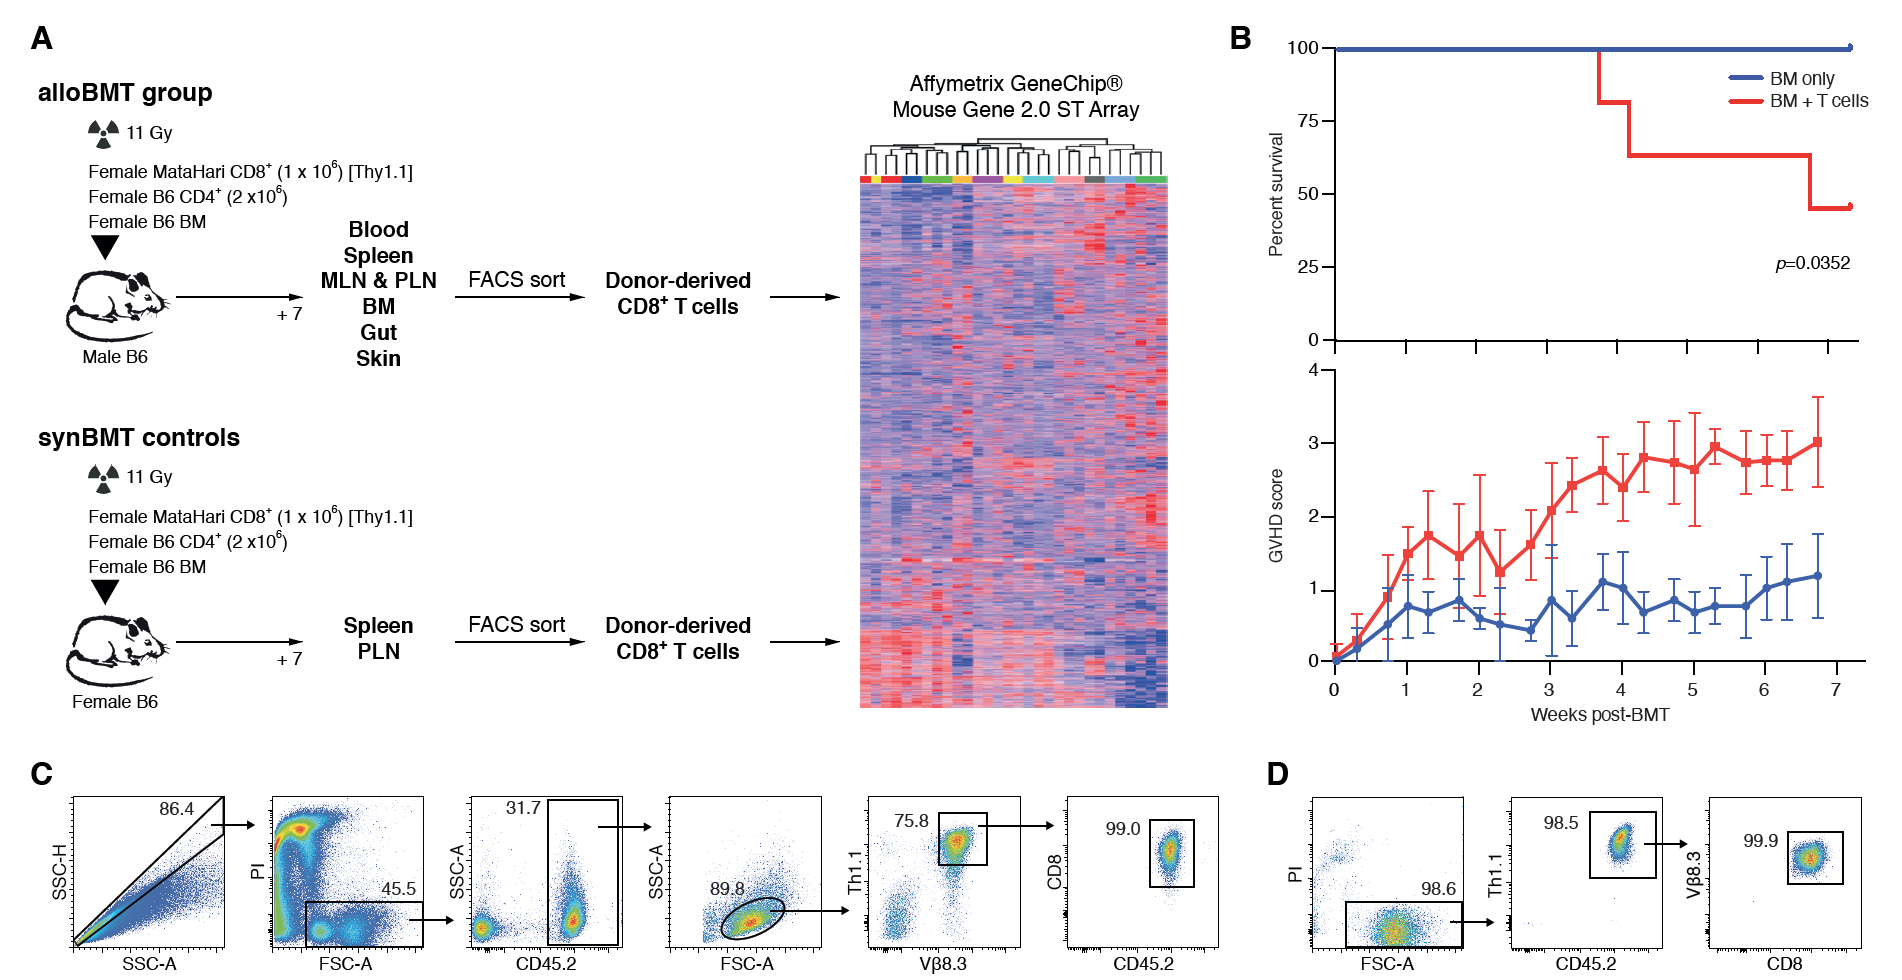
\includegraphics[width=0.9\textwidth]{Figures/Chapter1/MataHari.png}
   \caption{\small{\textbf{(A) Experimental setup.} Female MataHari CD8$\textsuperscript{+}$ T cells were transferred together with female B6 bone marrow and CD4+ T cells into lethally irradiated male B6 recipients (alloBMT group) or female B6 recipients (synBMT controls). Tissue harvesting took place at day +7 post-transplant and donor CD8$\textsuperscript{+}$ T cells were isolated and FACS sorted to high purity. Gene expression profile of sorted cells was assessed by whole-transcriptome microarray analysis. \textbf{(B) Characterization of the GVHD model.} Top graph: Kaplan Meier survival curve (log-rank Mantel-Cox test). Bottom graph: clinical GVHD score over time (mean ± SD). BM only (n=6), BM + T cells (n=11). \textbf{(C) Gating strategy used to sort donor derived CD8$\textsuperscript{+}$ T cells} (exclusion of doublets $\to$ exclusion of propidium iodide positive cells $\to$ exclusion of stroma cells $\to$ morphologic lymphocyte selection $\to$ selection of donor CD8$\textsuperscript{+}$ T cells based on the expression of congenic markers $\to$ confirmation of CD8 positivity). \textbf{(D) Gating strategy to evaluate purity at the end of each sort.} Abbreviations: BM, bone marrow; MLN, mesenteric lymph nodes; PLN, peripheral lymph nodes.} }
    \label{fig:1}
\end{figure}

\subsection{B6 into 129sv model}

\begin{figure}[H] 
    \centering
    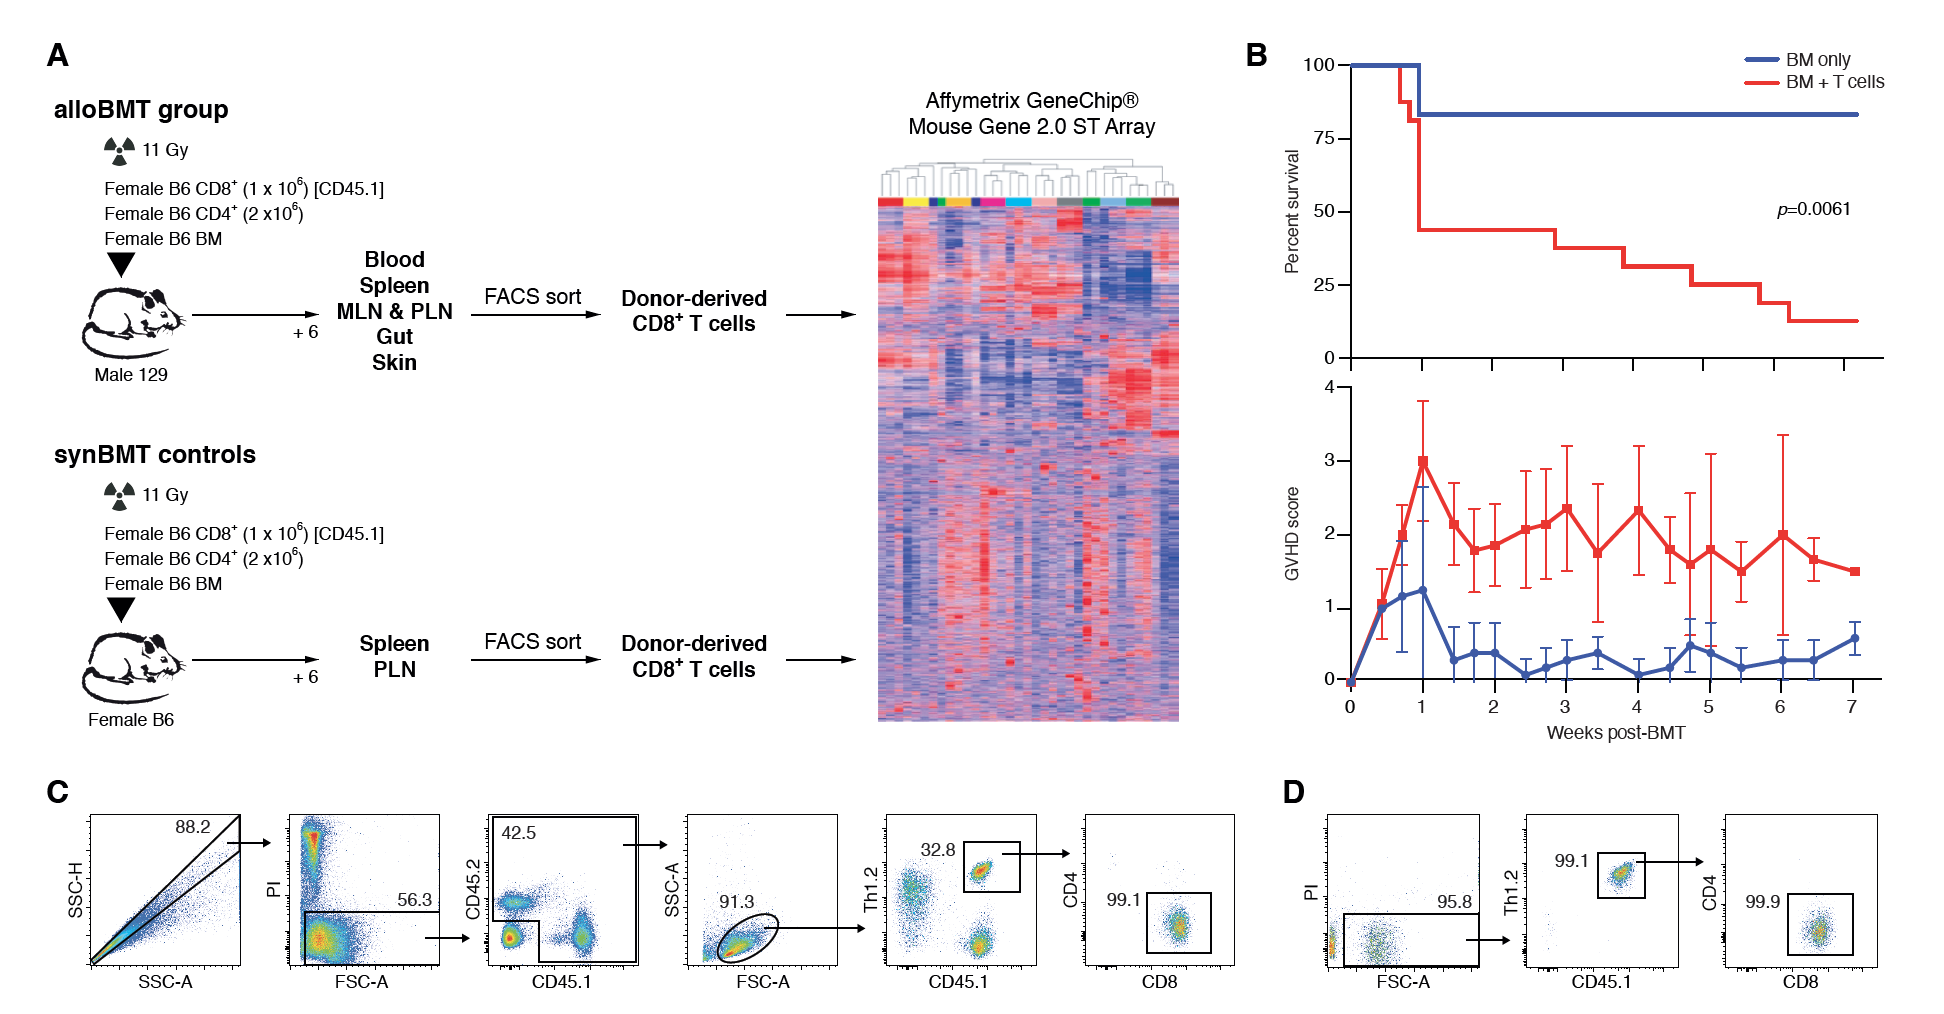
\includegraphics[width=0.9\textwidth]{Figures/Chapter1/B6_129.png}
   \caption{\small{\textbf{(A) Experimental setup.} Female B6 bone marrow and T cells were transferred into lethally irradiated male 129/Sv recipients (alloBMT group) or female B6 recipients (synBMT controls). Tissues were harvested at day +6 post-transplant and donor CD8$\textsuperscript{+}$ T cells were isolated and FACS sorted to high purity. Gene expression profiles of sorted cells was assessed by whole-transcriptome microarray analysis. \textbf{(B) Characterization of the GVHD model.} Top graph: Kaplan Meier survival curve (log-rank Mantel-Cox test). Bottom graph: clinical GVHD score over time (mean ± SD). BM only (n=6), BM + T cells (n=16). \textbf{(C) Gating strategy used to sort donor-derived CD8$\textsuperscript{+}$ T cells} (exclusion of doublets $\to$ exclusion of propidium iodide positive cells $\to$ exclusion of stroma cells $\to$ morphologic lymphocyte selection $\to$ selection of donor CD8$\textsuperscript{+}$ T cells based on the expression of congenic markers $\to$ confirmation of CD8 positivity). \textbf{(D) Gating strategy to evaluate purity at the end of each sort.} Abbreviations: BM, bone marrow; MLN, mesenteric lymph nodes; PLN, peripheral lymph nodes.} }
    \label{fig:2}
\end{figure}


\section{Systems biology approach}

Systems biology is perhaps best described as the adoption of a holistic approach to the task of understanding and interpreting complex biological systems. This field is based upon the premise that the whole is greater than the sum of the parts. In this context, "the whole" is often thought of as the networks that together from the living organism in its entirety. By it very nature this approach requires contribution from many scientific disciplines including biology, physics, computer science and bioinformatics to facilitate the exploration of new dimensions of data space and to tackle ever more challenging biological questions. 

As visualised in Figure 1.3, systems biology is usually thought of as a cyclical concept whereby new biological insights prompt the development of new, more powerful technologies to acquire increasing detailed data, which in turn necessitates the evolution of more advanced computational tools for appropriate analysis of the data obtained. Amongst other achievements, the ability to design predictive, multi-scale models now enables discovery of new biomarkers for disease, drug targeting as well as patient stratification based on unique genetic profiles.

\begin{figure}[H] 
    \centering
   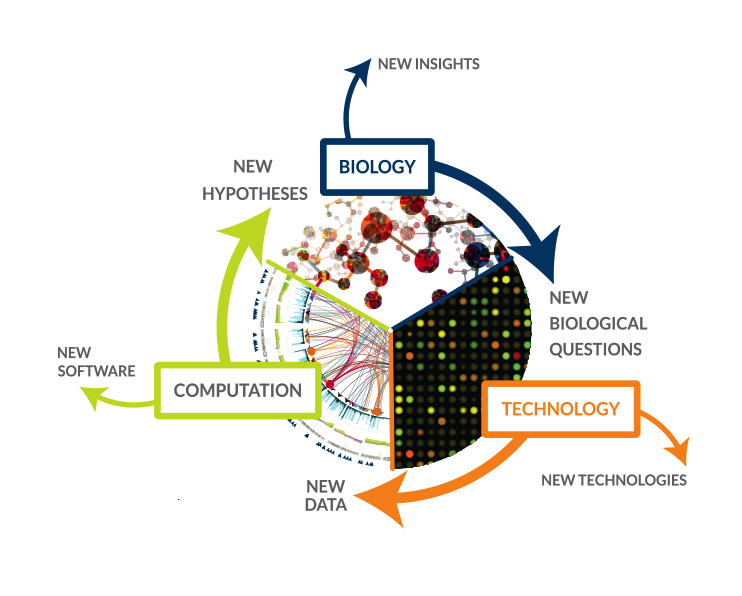
\includegraphics[width=0.8\textwidth]{Figures/Chapter1/systems_bio.jpg}
\caption{\small{The Institute for Systems Biology's depiction of how a cross-disciplinary environment allows for the establishment of a cycle where biology drives technology which in turn drives computation and so on.} }
    \label{fig:3}
\end{figure}

The high-throughput technologies in use today usually generate large lists of hundreds or thousands of potentially biologically interesting genes, but their biological interpretation is still a difficult task ~\autocite{Hua2009}. Indeed, there now exists a plethora of bioinformatics analytical/enrichment tools suitable for use with one or more of the currently available data types. Whilst this has undoubtedly been of huge benefit to thousands of research groups, the amount of choice can leave potential confused and overwhelmed regarding which is the best resource to meet their analytical requirements. It is often advisable for researchers to apply multiple tools from the same branch of analysis type to a given dataset and then manually compare the results and determine which offers the most biologically relevant insights ~\autocite{Hua2009}. In 2009, Huang \textit{et al.} performed a comprehensive analysis of the then available bioinformatics tools ~\autocite{Hua2009}. Although their list is now naturally very outdated, their classification of resources into three groups, namely singular enrichment analysis (SEA); gene set enrichment analysis (GSEA); and modular enrichment analysis (MEA), is still a valid separation. Briefly, SEA involves taking a pre-defined list of interesting genes, e.g. those found to be differentially expressed between case and control with a minimum 1.5 fold change, and linearly testing the enrichment of each known annotation term one-by-one. The major downsides of tools within this set are that the utility of the enrichment is heavily impacted by the quality of the pre-defined gene list and the output is often very large and not user-friendly. GSEA has a similar concept to SEA but with the key difference that GSEA takes as input all genes from a microarray experiment without pre-selection of significant genes. This naturally reduces the likelihood of analytical bias caused by prior determination of which genes are "interesting" and also means that even genes with seemingly small, but nonetheless interesting, changes in expression can still contribute to the analysis. Finally, MEA inherits the basic enrichment calculation found in SEA, but also incorporates network discovery algorithms by considering the term-to-term relationships. When considered together, these inter-relationships between enrichment terms may be of particular interest for the hypothesis under investigation and hence MEA will often produce results that are more easily related back to actual biological interactions than is the case for SEA or GSEA ~\autocite{Hua2009}.

As outlined in a previous section, our laboratory has generated two GVHD datasets using the B6 into 129sv and MataHari mouse models. Given the size and probable complexity of the microarray data obtained, we decided to utilise systems biology techniques to analyse these results and to try to identity clinically relevant gene modules that may help shed some light on the molecular pathways involved in the initiation and progression of GVHD in these mice. 

\subsection{Motivations: Benefit of clustering genes into modules?}

Virtually all cellular functions arise, at least on a fundamental level, as a direct consequence of gene expression patterns and subsequent protein-protein interactions. When considered at a more general level, these interactions can be seen to be organised into molecular pathways and feedback loops which together maintain homoeostatic functionality. Genes and the proteins they encode do not act in isolation but rather as part of one or more pathways or networks and hence it seems appropriate to analyse them in this context. Interconnected genes that form all or part of a biological network where nodes represent genes and edges the interactions between them, are often described as a gene module and it is these entitles that many bioinformatics tools try to identify by clustering together genes exhibiting similar patterns of expression ~\autocite{Lys2011}. These algorithms can be divided into many types based upon the mathematical premises they employ and include topology networks, network clustering, matrix decomposition and heuristic searches ~\autocite{Li2015}.

By attempting to identify gene modules within an expression dataset, we are far more likely to be in a position to understand the molecular implications of the condition/variable we are interested in than if we were to examine single, or even several genes, alone. However, this statement only holds true if the modules we identify and analyse are biologically meaningful and if one considers for a moment the detailed complexity of biological systems on every level, it can be seen that finding such modules is not as straightforward as it may initially appear. 

Many of the clustering algorithms developed to date group genes based on correlation networks between expression profiles as measured by microarray, or similar, techniques. These quantitative analyses typically produce measurements which can be described by an \textit{n} by \textit{m} matrix as follows: 

\begin{equation}
X = |x_ {il}|
\end{equation}

where the row indices correspond to network nodes (\textit{i} = \textit{1, 2,... n}) and the column indices (\textit{l} = \textit{1, 2,.. m}) correspond to sample measurements ~\autocite{Lan2008}. This can be written in the form:

\begin{equation}
\mathbf{X = |x_ {ij}|} = \left(
\begin{array}{c}
x_\textit{1} \\
x_\textit{2} \\
\vdots \\
x_\textit{n}
\end{array} \right)
\end{equation}

We refer to the \textit{i}-th row $x_i$ as the \textit{i}-th node profile across \textit{m} sample measurements. 

The rationale behind correlation network methodology, which is a common analytical choice among biologists, is to use network language to describe the pairwise relationships (correlations) between the rows of X ~\autocite{Lan2008}.

\subsection{How to evaluate quality of clustering results}

With advances in the development of stable gene clustering algorithms, researchers are now faced with questions of how to evaluate the accuracy and validity of modules they identify. However, given the prevalence of such algorithms, there are still surprisingly few established methods for the validation and evaluation of module gene sets. Until fairly recently, aside from size-limited experimental techniques to verify interactions between module members, studies largely relied upon function enrichment tools e.g. Gene Ontology (GO) and KEGG to determine the quality of their modules through enrichment. However, this method rarely produces evenly annotated modules and should theoretically be periodically re-analysed to account for updates made to the annotation database itself ~\autocite{Li2015}. 

In response to these shortcomings, research focus is now shifting to incorporate computational methods into the standard module validation analysis protocols. Such techniques often involve the probing of a modules architectural properties and collectively are sometimes known as Computational Validation Approaches based on Modular Architecture (CVAMA). CVAMA are suitable for application to modules of any size and are not reliant on external databases. In their recent review Li \textit{et al.} divided available CVAMA methods into topology-based approaches (TBA) and statistics-based approaches (SBA) and in the following brief summary we echo their distinctions ~\autocite{Li2015}. 

\subsubsection{topology-based approaches (TBA)}

A gene module can be seen as possessing several network topological features which can be used to quantify its physical parameters. Most analytical projects will tend to focus on one or several of these criteria which are deemed by the researchers to be most relevant for the purpose of establishing whether the proposed modules possess a non-random structure ~\autocite{Don2012}. Here we provide a list of typical parameters examined together with their definitions which have been taken from review of this topic by Doncheva \textit{et al.}~\autocite{Don2012}:

\paragraph{Connected components -} 
When considering an undirected network, any two given nodes are said to be connected if there are one or more edges between them. This parameter provides an indication of global connectivity, with a low value suggesting a strongly connected network.

\paragraph{Degree distributions -} 
For undirected networks, the node degree of a node \textit{n} is the number of edges to which it is linked. The \underline{node degree distribution} gives the number of nodes with degree \textit{k} for \textit{k = 0, 1, etc.} Nodes with high values of \textit{k} are known as hubs. In directed networks, the "in-degree" of node \textit{n} is the number of incoming edges and the "out-degree" is the number of outgoing edges. A network is termed scale-free if its degree distribution approximates a power law $k^{-\alpha}$ with the degree exponent \textalpha. As a general rule for biological studies, hubs with $\alpha >$ 3 are classed as irrelevant, those where 3 $< \alpha >$ 2 tend to possess hierarchical organisation and when $\alpha =$ 2 a 'hub-and-spoke' model (referring to the connectivity of the largest hub) is often seen. In the case of biological networks $\alpha$ is commonly between 2 and 3.

\paragraph{Neighbourhood-related parameters -} 
The set of neighbours for a particular node \textit{n} comprises its neighbourhood. The \underline{connectivity} \textit{kn} is the size of the neighbourhood of \textit{n} and the average of one can give an approximation of the average of the other. A networks density is a normalised version of this parameter. A network without any edges will have a density of 1, while the value for a clique will be 1.

\paragraph{Neighbourhood Connectivity} 

As mentioned above, the \underline{connectivity} of a node \textit{n} is the number of its neighbours. As such the neighbourhood connectivity of node \textit{n} is defined as the average connectivity of all neighbours of \textit{n}. The corresponding \underline{neighbourhood connectivity distribution} summarises the average of the neighbourhood connectivities of all nodes \textit{n} with \textit{k} neighbours for \textit{k = 0, 1, etc.} For directed networks, any given node possess three types of neighbourhood connectivity:

\begin{itemize}
    \item \emph{Only in }- the average out-connectivity of all in-neighbours of \textit{n}
    \item \emph{Only out }- the average in-connectivity of all out-neighbours of \textit{n}
    \item \emph{In and out} - the average connectivity of all neighbours of \textit{n}, where edge direction is ignored
\end{itemize}

Based on these definitions there are three equivalently named neighbourhood connectivity distributions.

\paragraph{Shortest paths -}

The length of a path is represented by the number of edges forming it. The length of the shortest path, or distance, between two nodes \textit{n} and \textit{m} is denoted by L(\textit{n,m}). The \underline{shortest path length distribution} gives the number of node pairs (\textit{n,m}) with L(\textit{n,m}) = \textit{k} for \textit{k = 0, 1, etc.} The \underline{eccentricity} of a node \textit{n} is the maximum non-infinite length of a shortest path between \textit{n} and another node in the network. The \underline{network diameter} is the maximum node eccentricity. 

the \underline{network radius} is defined as the minimum of the nonzero eccentricities of the nodes in the network. The \underline{average shortest path length} gives the expected distance between two connected nodes.

\paragraph{clustering coefficients -}

In undirected networks, the clustering coefficient $C_n$ of a node \textit{n} is defined as $C_n = 2e_n/(k_n(k_n–1))$, where $k_n$ is the number of neighbours of \textit{n} and $e_n$ denotes the number of edges between all neighbours of \textit{n}. In directed networks, this coefficient is parametrised by $C_n = e_n/(k_n(k_n–1))$. 

In both instances, the clustering coefficient is a ratio \textit{N/M}, where \textit{N} is the number of edges between the neighbours of \textit{n}, and \textit{M} the maximum number of edges that could possibly exist between the neighbours of \textit{n}. For any given node \textit{n}, this value is always between 0 and 1. 

The \underline{network clustering coefficient} is the average of the clustering coefficients of all nodes in the network and the \underline{average clustering coefficient distribution} gives the average of the clustering coefficients for all nodes \textit{n} with k neighbours for \textit{k = 2, 3, etc}.  

\paragraph{Shared neighbours -}

Defined as \textit{P}(\textit{n,m}), this parameter represents the number of interaction partners shared between nodes \textit{n} and \textit{m}. The \underline{shared neighbours distribution} gives the number of node pairs (\textit{n,m}) with \textit{P}(\textit{n,m}) = \textit{k} for \textit{k = 1, 2, etc}. 

\paragraph{Topological coefficients -}

The topological coefficient $\textit{T}_n$ of a node \textit{n} with $\textit{k}_n$ neighbours is computed as: 

\begin{equation}
\textit{k}_n = avg (\textit{J}(\textit{n, m}))/\textit{k}_n
\end{equation}

Here \textit{J}(\textit{n, m}) is defined for all nodes \textit{m} that share at least one neighbour with \textit{n}. 
The value \textit{J}(\textit{n, m}) is the number of neighbours shared between the nodes \textit{n} and \textit{m}, plus 1 if there is an edge between \textit{n} and \textit{m}. This coefficient is a relative measure for the extent to which a given node \textit{n} shares neighbours with other nodes. 

\paragraph{Stress centrality -}

The stress centrality of a given node \textit{n} is the number of shortest paths passing through \textit{n}. The \underline{stress centrality distribution} gives the number of nodes with stress \textit{s} for \textit{s = 1, 2, etc}. 

\paragraph{Betweenness centrality -}

The betweenness centrality $C_b\textit{(n)}$ of a node \textit{n} is defined as:

\begin{equation}
C_b\textit{(n)} = \textstyle \sum_{s\neq n\neq t}^{}  (\sigma_{st}(n)/\sigma_{st})
\end{equation}

where, \textit{s} and \textit{t} are nodes in the network other than \textit{n}, $\sigma_{st}$ gives the number of shortest paths from \textit{s} to \textit{t}, and $\sigma_{st}(n)$ is the number of shortest paths from \textit{s} to \textit{t} that pass through \textit{n}.

This parameter is only computed when a network is comprised of single edges alone. 

The betweenness value for each node \textit{n} is normalised to lie between 0 and 1 by dividing the number of node pairs excluding \textit{n} as follows:
\begin{equation}
(\textit{N} -– 1)(\textit{N} -– 2) / 2
\end{equation}
 where \textit{N} is the total number of nodes in the connected component that \textit{n} belongs to. The betweenness centrality of a node reflects the amount of control it exerts over the interactions of other nodes in the network.

\paragraph{Closeness centrality -}

The closeness centrality $C_\textit{(n)}$ of a node n is the reciprocal of the average shortest path length. The closeness centrality of each node \textit{n} is a value between 0 and 1 and is a measure of how quickly information spreads from a given node \textit{n} to other reachable nodes in the network.

Several topological indexes have also been developed to evaluate a given module's likely validity. These include the the network perplexity index of Entropy where a good quality module is expected to have a low entropy ~\autocite{Zha2009}. This index is typically defined as follows: 

\begin{equation}
Entropy (M) = -\textstyle \sum_{J \in {bins}}^{} P_j log_2 P_j
\end{equation}

Another widely used single index is the NB Value which is used to identify modules with high intra-modular connectivity (NB $\geq$ 0.5) ~\autocite{Oza2010}. The NB Value represents a ratio of edges within a module and the total number of edges between modules:

\begin{equation}
NB = \frac{\sum e(i)} {\sum d(i)} 
\end{equation}

To be of informative value it is vital that the index chosen to validate a module should be independent of the methods used to identify the module. It is also common practice for multiple topological indexes or module preservation statistics to be combined into an integrated measure for the overall assessment of module validity or preservation. Perhaps the most widespread composite preservation statistic used to validate whether a module is significantly preserved in another network is the Z\textsubscript{summary} score ~\autocite{Lan2011}: 

\begin{equation}
Z_{summary} = \frac{Z_{density} + Z_{connectivity}} {2} 
\end{equation}

A Z\textsubscript{summary} score of $\geq$ 10 indicates that a module is strongly preserved, a value between 2 and 10 suggests moderate preservation and if this index produces a score $\leq$ 2 then no preservation is found. 

\subsubsection{statistics-based approaches (SBA)}

As well as exhibiting some form of modular structure which can be analysed using the topological criteria detailed above, a "good" gene module should be statistically significant i.e. its architecture distribution ought to be very unlikely to be obtained by chance in a randomised network. It is often also important to quantify relationships between modules and phenotypic characteristics and this too requires some measurement of statistical significance. Depending on the biological context it is possible to use binary or mixed integer linear models to validate causal or dependent relationships between network modules and biological phenotypes ~\autocite{Hen2011,Sch2011,Shi2010}. Using a permutation test with a \textit{p}-value calculated by estimating the null distribution we are able to determine whether the composition of a given module is higher than expected by chance or is associated with a particular disease phenotype ~\autocite{Jia2012}. As mentioned above, comparative network analysis techniques such as Z\textsubscript{summary} can also aid the identification of conserved modules across networks or species, as well as providing insight into the reproducibility of the module in question. 


\subsection{Two complementary approaches to module definition}

\subsection{Prior generation of MataHari modules using WGCNA}

To tackle the hypothesis mentioned previously, i.e. to measure the respective roles of lymphoid organs and peripheral tissues in dictating T cell effector programs that result in tissue injury, our team began by characterising the transcriptional response of donor CD8$\textsuperscript{+}$ effector T cells as they trafficked to multiple sites during the evolution of GVHD. This enabled the analysis of how T cells differentiate within secondary lymphoid organs (SLO) compared to those in peripheral tissues. Experiments using the MataHari and B6 into 129sv GVHD models were performed as outlined in Figures 1.1 and 1.2 respectively. Once microarray data had been acquired from the B6 into 129sv experiments, skin- and gut-tissue specific genes, determined using PaGenBase, were removed from the datasets to correct for any contamination by other celltypes. Multi-dimensional scaling (MDS) was performed on both datasets and as evidenced by Figure 1.4A, not only do allogeneic recipients segregate separately from both na\"ïve T cells and those undergoing proliferation within lymphatic tissues, but there is also a clear distinction within recipients of allogeneic BMT between those T cells deriving from secondary lymphoid organs (plotted as blue circles) and those within GVHD target tissues (shown as red circles in the plot). 

\begin{figure}[H] 
    \centering
   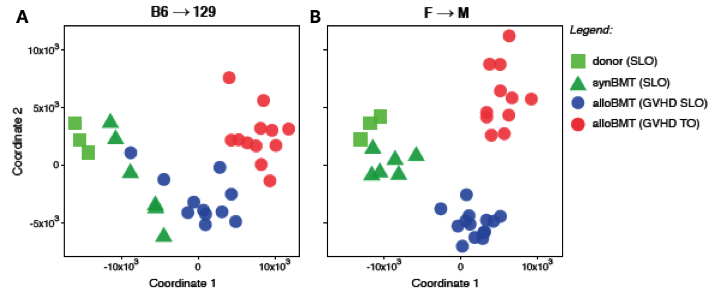
\includegraphics[width=0.8\textwidth]{Figures/Chapter1/lab_MDS_plot.png}
\caption{\small{Multi-dimensional scaling (MDS) plots depicting the proximity of the transcriptional profiles of donor derived CD8$\textsuperscript{+}$ T cells isolated from the spleen, lymph nodes, blood, gut and skin, in the two model systems (B6 into 129sv and MataHari Female $\to$ Male).} }
    \label{fig:4}
\end{figure}

It was concluded that these observed differences in gene expression profiles could be the result of either tissue environment-dependent re-programming or the selection of pre-existing variants from the bulk population. To exclude the latter option the experiments were repeated in the MataHari B6 female $\to$ B6 male. This BMT model involves the transfer of na\"ive MataHari CD8$\textsuperscript{+}$ T cells transgenic for a TCR that recognises a single, ubiquitous HY antigen, Db-Uty. As can be seen in Figure 1.4B, the expression profiles of T cells found in GVHD target organs are again clustered away from those in the secondary lymphoid organs. Additionally, there was a substantial amount of overlap identified between effector T cell expression profiles from each tissue in the MataHari Female $\to$ Male dataset and the equivalent sample in the B6 into 129sv model which supports the theory that differences in effector T cell profiles reflected the source tissue and were independent of the T cell receptor repertoire. Given the profound separation seen between tissue groups in the MataHari Female $\to$ Male model, this dataset was taken forward for further analysis. 

Using the analytical method Weighted Gene Correlation Network Analysis (WGCNA), which is detailed in Chapter \ref{Chapter3}, modules of co-expressed genes were identified within the Female $\to$ Male data in the hope that they may assist in gaining an understanding how tissue specific effector T cell transcriptional programs develop. A total of 31 such gene modules were found and the inter-module expression patterns were seen to vary substantially between both the type of BMT (syngeneic or allogeneic) and the tissue source of the T cells. This diversity in module expression profiles, which is portrayed in Figure 1.5A, even extended to tissue sub-compartments (e.g. the dermis versus the epidermis). As evidenced by this Figure, a marked distinction was observed between those modules up-regulated in GVHD target organs compared to the secondary lymphoid organs which is of great interest given our hypothesis of tissue specific re-programming of effector T cells. In order to determine how well these 31 modules were conserved in the B6 into 129sv model the Z\textsubscript{sum} composite preservation measurement was used. Of the 31 modules identified in the Female $\to$ Male dataset 30 were found to be conserved in the B6 into 129sv dataset based on a Z\textsubscript{sum} > 2.0, while 19 modules passed the cut-off at Z\textsubscript{sum} > 10. These 19 modules were subsequently annotated to identify enriched biological processes using the Gene Ontology database ~\autocite{Ash2000,GO2015} and candidate driver genes i.e. genes exhibiting high intra-modular connectivity were pinpointed. The most significant biological process annotations and likely driver genes are shown in Figure 1.5B. 

\begin{figure}[H] 
    \centering
   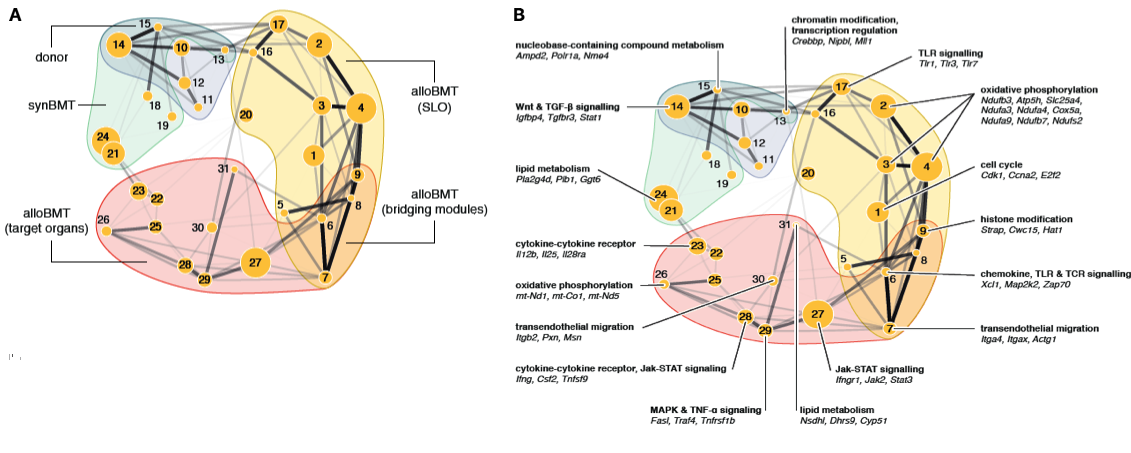
\includegraphics[width=0.9\textwidth]{Figures/Chapter1/MH_mods.png}
\caption{\small{A. Summary Eigengene network where shaded areas represent MataHari Female $\to$ Male module clusters associated with the surveyed experimental groups and GVHD subgroups. B. MataHari Female $\to$ Male modules classified according to the main classes of Gene Ontology terms of the annotated genes. Putative driver genes for each conserved module were identified on the basis of high intra-modular connectivity (3 examples per module).} }
    \label{fig:5}
\end{figure}

Further details and discussions of these findings will not be included here but given the importance of this dataset for work presented later in this report, the following represents a summary of the authors primary observations: 

\begin{enumerate}
    \item Several, strongly interconnected gene clusters segregated primarily with the SLO origin of effector T cells e.g. M17 was strongly correlated with T cells from the LN but negatively correlated with those of GVHD target organs; 
    \item M1 which contains genes associated with DNA replication and the cell cycle mapped to blood and BM-derived effector T cells;
    \item M3 segregated with the spleen and BM TE and was almost exclusively comprised of fatty acid oxidation and oxidative phosphorylation related genes;
    \item M7 which contained genes encoding proteins implicated in cytoskeletal reorganisation and transendothelial migration was the most densely interconnected of the bridging modules;
    \item  The largest GVHD target organ-specific module was M27. This module was enriched for multiple intracellular signalling gene pathways including MAPK and JAK-STAT;
    \item M28 was highly specific for effector T cells of the epidermis and contained a strong Ifng-related signal with genes for multiple pro-inflammatory cytokines, cytokine receptors and downstream adaptors;
    \item  M29 segregated with the majority of GVHD target organs and is considered by the authors to represent a pan-GVHD target organ gene cluster;
    \item  Driver genes identified within the M7, M28 and M29 modules, showed a high degree of overlap with a Th1/17-related pathogenicity gene cluster that is linked to aggressive T cell autoimmunity
\end{enumerate}
 
It can thus be seen that this MataHari dataset together with the WGCNA-derived gene modules discussed briefly above represent a highly useful and detailed resource from which we can potentially learn much regarding the impact of tissue specific effector T cell imprinting on GVHD pathology. 
 
 %input each chapter as a seperate .tex files
% Chapter 1

\chapter{Introduction} % Main chapter title

\label{Chapter1} % For referencing the chapter elsewhere, use \ref{Chapter1} 

%----------------------------------------------------------------------------------------

% Define some commands to keep the formatting separated from the content 
\newcommand{\keyword}[1]{\textbf{#1}}
\newcommand{\tabhead}[1]{\textbf{#1}}
\newcommand{\code}[1]{\texttt{#1}}
\newcommand{\file}[1]{\texttt{\bfseries#1}}
\newcommand{\option}[1]{\texttt{\itshape#1}}

%----------------------------------------------------------------------------------------
\section{Graft versus Host Disease}
\subsection{Clinical Background}

Allogeneic hematopoietic stem cell transplant (HSCT) represents the primary treatment for multiple malignant and nonmalignant diseases that would often prove fatal without intervention. However the current efficacy of HST is hampered by the fact that many patients go on to develop Graft-versus-Host Disease (GVHD), a condition that represents the most serious and life threatening complication to arise from this treatment with an overall mortality rate of 15\% ~\autocite{Fur2015, Bla2012}. Prior to HSCT, recipients undergo a conditioning regimen that is not only myelosuppressive to deplete the host immune system and facilitate donor stem cell engraftment, but is also immunosuppressive thus reducing the likelihood of graft rejection ~\autocite{Bla2012}. Indeed it is the toxicity and suppressive effects of this regimen that, by precipitating tissue damage and inflammation in the host, can lead to the development of clinical GVHD. This pre-HSCT conditioning usually takes the form of chemotherapy and is followed by the transfer of a stem cell graft. CD4+ and CD8$\textsuperscript{+}$ T cells are often co-transplanted with the graft and represent the primary immunocompetent population of cells that mediated a beneficial anti-tumour response known as Graft-versus-Leukaemia (GVL) ~\autocite{Pac2013}, also referred to as Graft-versus-Tumour (GVT) and promote haematopoietic engraftment. However, these cells also induce GVHD ~\autocite{Cha2007}. Development and severity of the disease depend on multiple factors such as recipient age, toxicity of the conditioning regime, haematopoietic graft source and GVHD treatment approaches which will be discussed in more detail later in this text ~\autocite{Bla2012}.

Put simply, GVHD occurs when immune cells transplanted from a non-identical donor (the graft) recognise host tissues in the transplant recipient as foreign and initiate an immune reaction that causes multi-system disease in the transplant recipient. Despite the prevalence of this disease variation in the identification, documentation and measurement of acute GVHD in particular means that obtaining accurate estimates of incidence in a given cohort are often not available. Historically GVHD has been divided into two subtypes namely acute and chronic based purely on time of manifestation; with acute GVHD defined as that occurring within 100 days of transplantation ~\autocite{Buz2008}. Mortality rates have been shown to be as high as 90\% for patients with steroid-refractory acute GVHD while the chronic subtype is associated with a 5 year mortality rate of 30-50\% ~\autocite{Bla2012}. In addition to differing times of onset it has since been demonstrated that acute GVHD and chronic GVHD involve distinct pathological processes and have characteristic clinical presentation ~\autocite{Bla2012}. While acute GVHD has strong inflammatory components and often presents with symptoms including a maculopapular rash, persistent nausea, diarrhea and a rising serum bilirubin concentration, chronic GVHD displays more autoimmune and fibrotic features such as skin involvement resembling lichen planus or the cutaneous manifestations of scleroderma together with ulcerations and sclerosis of the gastrointestinal tract. Immune dysregulation and opportunistic infections have been shown to be the primary causes of death among chronic GVHD patients ~\autocite{Bla2012}. There exists substantial evidence to support the above classifications but this division has been called into question by recognition of the fact that signs of acute and chronic GVHD may occur outside of the designated periods mentioned above. This has led to the increased use of clinical findings, rather than time periods, to distinguish acute from chronic GVHD. In line with this the National Institutes of Health (NIH) have put in place the following criteria to sub-classify GVHD: 
\begin{itemize}
    \item Classic acute GVHD - Cases present within $100$ days of hematopoietic cell transplant (HCT) and display features of acute GVHD. Diagnostic and distinctive features of chronic GVHD are absent.
    \item Persistent, recurrent, late onset acute GVHD - Cases present greater than $100$ days post-HCT with features of acute GVHD. Diagnostic and distinctive features of chronic GVHD are absent.
    \item Classic chronic GVHD - Cases may present at any time post-HCT. Diagnostic and distinctive features of chronic GVHD are present. There are no features of acute GVHD.
    \item Overlap syndrome - Cases may present at any time post-HCT with features of both chronic GVHD and acute GVHD. On occasion, this is colloquially referred to as "acute on chronic" GVHD.
\end{itemize}

The pathophysiology of acute GVHD is typically divided into three distinct phases. The first of these occurs during conditioning when host tissues are damaged by the given regimen (irradiation and/or chemotherapy), thus triggering their activation. This in tern leads to the secretion of inflammatory cytokines TNF-a and IL-1 and a consequential increase in expression of MHC antigens. In the second stage, following transfer into irradiated allogeneic recipients, na\"ive donor T cells are initially retained within secondary lymphoid tissues such as the lymph nodes and spleen. Here they undergo rapid proliferation before entering the peripheral circulation 3-4 days later ~\autocite{Cha2007}. Once released from secondary lymphoid tissues, donor T cells are activated by the recognition of host alloantigens and subsequently proliferate, differentiate and secrete cytokines such as IL-2. The signalling cascade that results ultimately causes the recruitment of effector cells to target organs e.g. the skin ~\autocite{Red2003}. Finally, in stage three, effector functions of cytotoxic T cells cause damage to host target tissues and acute GVHD becomes clinically evident ~\autocite{Buz2008}. This tissue specific damage leads to the involvement of other effector cells e.g. natural killer (NK) cells and neutrophils which further augment tissue injury ~\autocite{Bla2012}. The critical importance of T cells in acute GVHD pathology has been heavily supported by the complete abrogation of GVHD following T cell depletion from the graft. Indeed, to date this strategy remains the most effective in preventing acute GVHD. There remain many unresolved questions regarding the precise mechanisms and celltypes involved in the activation of T cells. These uncertainties will be discussed later but are primarily focused on whether cross-presentation of antigen by donor antigen presenting cells (APCs) can cause activation of T cells and initiation of acute GVHD ~\autocite{Cha2007}. When compared to the acute subtype, the pathophysiology of chronic GVHD is seemingly more complex and we still know relatively little about it. Current theories based on available data include aberrant Transforming Growth Factor-\textbeta (TGF-\textbeta), thymic damage during pre-transplant conditioning and consequentially defective negative selection of T cells, deficiencies in regulatory T cells (Tregs) and auto-antibody production ~\autocite{Aro2010}.

Currently there exist no laboratory tests that can predict either the risk of a patient developing GVHD post HSCT, or likely responsiveness to treatment and survival prognosis. The fact that diagnosis is almost soley based upon the existence of clinical symptoms and biopsy of the target organ involved represents a significant barrier to GVHD research and treatment advancement. The development of accurate biomarkers to identify patients at high risk of developing this complication at an early stage of the transplantation/treatment process is of great importance in the improvement of therapeutic protocols and development of tailored treatment plans ~\autocite{Pac2013}. Should such a diagnostic test exist it would ideally need fulfil several criteria. Firstly, it must accurately distinguish cases of GVHD from those suffering a separate complaint e.g. gastrointestinal GVHD \textit{cf.} infectious colitis. Secondly, a successful biomarker should enable classification of the current disease state. In addition the test itself would need to be quick, inexpensive,  non-invasive and perhaps most importantly standardised. It would naturally be advantageous if the same diagnostic test was also able to give an indication of probable prognosis in terms of survival, NRM and treatment success. Statistics such as these could facilitate risk stratification of patients prior to the commencement of treatment. As discussed by Paczesny ~\autocite{Pac2013}, biomarkers for GVHD largely fall into the following three categories: 
\begin{itemize}
    \item MicroRNAs - 21-25 nucleotide transcripts that repress gene function via interactions with target messengerRNAs.
    \item Cellular biomarkers - These utilise the fact that the functions and numbers of several different immune cell populations e.g. regulatory T cells (Tregs) are altered in GVHD and can be used as biomarkers for this pathology. 
    \item Proteomic biomarkers - the proteome is defined as the totality of proteins present in a sample at a given time point. For this reason proteins are an ideal choice of biomarkers in post-transplantation conditions. It can therefore be argued that the optimal location to search for biomarkers is likely to be within the target tissues themselves but this has so far proved difficult due to limited tissue sample sizes and issues of cellular heterogeneity. 
\end{itemize}

Once a diagnosis of GVHD has been made, treatment with steroids and/or broad-spectrum antibiotics is the most common course of action. The downside of such treatments is that as they are non-specific in their targeting of T cells, they will more than likely have a substantial negative impact on GVT and immune reconstitution ~\autocite{Bla2012}. There is still some debate regarding the precise nature of the relationship between GVT and GVHD but Storb \textit{et al.} reported increased GVT in patients with chronic GVHD by no association was seen for patients suffering from the acute form of the condition ~\autocite{Sto2013}. Indeed, multiple studies have highlighted that transplant patients with chronic GVHD have a decreased relapse risk compared to those who do not develop any form of GVHD, although this potential benefit is unfortunately usually found to be offset by higher instance of non-relapse mortality.

One comparatively recent development in the treatment of GVHD is the incorporation of regulatory T cells (Tregs) into conditioning regimes. There is some evidence that administration of CD4+CD25+ Tregs counteracts the GVHD causing potential of donor alloreactive T cells without interfering with the expansion of co-infused T cells possessing a broad T cell receptor (TCR) repertoire ~\autocite{Ian2015}. This ensures long-term immunity and protection from diseases such as CMV. Although the long term effects of this prophylactic approach are yet to be determined, it is thought that in an inflammatory environment transferred Tregs are activated by recipient APCs and block the activity of alloreactive T cells in an antigen-specific manor ~\autocite{Ian2015}. Attempts to reduce the intensity of conditioning regimens e.g. using non-myeloablative conditioning regimens or to localise the treatment using techniques such as total lymph node irradiation have also led to a reduction in the incidence of acute GVHD as well as improved treatments but these regimens are heavily reliant on GVT effects to eliminate residual malignant cells ~\autocite{Bla2012}.

To date, the majority of preclinical studies into GVHD pathogenesis have been performed in mice. This includes studies undertaken within our laboratory, the results of which form the primary datasets for this project. However, substantial insights, notably into effects of pharmacological agents, have also been gleaned from studies in large animal models e.g. canine and nonhuman primates ~\autocite{Bla2012}. It has been demonstrated that the period of engraftment represents the optimal point at which to examine gene expression changes duration acute GVHD ~\autocite{Buz2008} but whether this is appropriate is of course dependent upon the nature of the hypothesis being tested. 

\subsection{Risk factors}
As our awareness of the prevalence and potential severity of GVHD has grown, so too has our understanding of the risk factors that contribute to the likelihood of an individual developing this condition. Whilst there appears, unsurprisingly, to be some overlap when it comes to comparing known risk indicators for acute and chronic GVHD subtypes, not all studies currently concur with respect to the impact of some factors. 

Among risk factors for acute grades 2-4, the most well described include recipient human leukocyte antigen (HLA) mismatching with the donor, use of a female donor for male HSCT recipients, older patient age at time of HSCT and alloimmunization of the donor ~\autocite{Flo2011}. Interestingly, using rabbit ATG during the conditioning regimen has been shown to be linked to a reduced risk of developing acute GVHD, possibly by inhibiting activation of donor T cells or causing their depletion ~\autocite{Flo2011}. Some have additionally found that incorporating high intensity irradiation into pre-transplant conditioning, donor age and prior cytomegalovirus (CMV) infection in the recipient although there exist multiple conflicting reports concerning the impact of the latter factor in particular ~\autocite{Hah2008}.

Turning to chronic GVHD, prior acute GVHD, older patient age at time of transplant, grafting with growth factor-mobilized blood cells, sex-mismatch of donor for male recipients, older patient age, and HLA mismatched/unrelated donors have all been found to correlate with increased risk of disease ~\autocite{Flo2011}. Rabbit ATG has again been shown to associate with a reduction in the probability of a patient acquiring chronic GVHD but the biological mechanisms underlying this phenomenon remain poorly understood. A decrease in thymic damage resulting in better negative selection of alloreactive T cells is one plausible explanation ~\autocite{Flo2011}. In recent years genetic profiling of both HSCT donors and recipients have highlighted the importance of the expression patterns of certain genes by CD4$\textsuperscript{+}$ and CD8$\textsuperscript{+}$ T cells of the donor in quantifying the risk of developing post-transplant complications. Baron \textit{et al.} have found that the activities and interactions of multiple genes in donor T cells responsible for the regulation of cellular functions including proliferation and TGF-\textbeta signalling are associated with the development of chronic GVHD following HSCT accompanied by high dose conditioning ~\autocite{Bar2007}. This finding has particular clinical relevance as others have reported the attenuation of GVHD following early post-transplant TGF-\textbeta production in donor T cells and this cytokine is known to possess tumour suppressive capacities in the context of haematologic pathologies. The same study also uncovered a potential link between TCIRG1 and reduced risk of GVHD. This gene codes for the \textalpha 3 subunit of vacuolar H+-ATPase which colocalizes with the T cell receptor and mediates inhibitory signals that lead to up-regulation of CTLA4 and repression of interleukin-2 and its upregulation has previously been shown to increase both kidney and heart graft lifespan ~\autocite{Bar2007}.

It is therefore important to note that although GVHD is known to result from donor T cell responses to host alloantigens, disease manifestation and severity are not determined by histoincompatibility alone. This has been neatly demonstrated in both human and mouse models using major histocompatibility complex(MHC)-identical individuals or inbred strains respectively. Given that such individuals display over 50 minor histocompatibility antigen differences, if histoincompatibility was sufficient to induce GVHD the expected disease occurrence would be 100\%.  Instead it has been shown as being 50\% in mice and 73\% for human recipients ~\autocite{Bar2007}. One concept which is yet to be explored in depth is that of the inherent immune responses of the donor. It is logical that variations in these responses, partially the result of past infections encountered, may lead to some individuals being 'stronger alloresponders' and thus potentially more likely to trigger GVHD when transferred to the host ~\autocite{Bar2007}. Appropriate quantification of gene expression signatures may shed light on this aspect of HSCT transplant biology.  This area of research is even more intriguing when viewed in light of the observation that the donor CD4$\textsuperscript{+}$ and CD8$\textsuperscript{+}$ T cell gene expression profiles seem to persist in the recipient after transfer. Baron \textit{et al.} state that in their study of microarray data, the gene profile of the donor T cells on day 0 was highly correlated with the recipients on day 365 post-HSCT ~\autocite{Bar2007}. It is well documented that by this time point post transplant recipient T cells derive predominatly, if not entirely, from the differentiation of donor-derived hematolymphoid progenitors in the thymus of the recipient and this has lead to the theory that differing donor gene profiles are imprinted in hematopoietic stem cells ~\autocite{Bar2007}.

It can be seen from the above that there is evidence that acute and chronic GVHD represent distinct syndromes with separate pathologies as mentioned above. Indeed the fact that both mobilized blood cells grafts and older patient age seem to translate into an increased risk of chronic GVHD but not acute GVHD supports this conclusion ~\autocite{Flo2011}. Furthermore, the results of Baron \textit{et al.} suggest that of the genes they identified as being associated with GVHD risk, 54\% and 62\% of CD4$\textsuperscript{+}$ and CD8$\textsuperscript{+}$ specific signatures respectively correlated with only one GVHD subtype ~\autocite{Bar2007}. Thus it seems logical to conclude that based upon current evidence acute and chronic GVHD should be classed as separate entities. 

\subsection{SNPs implicated in GVHD pathology}

It has been known since the time of some of the earliest transplants that genetic variation between individuals involved in an HSCT could induce immune responses in the recipient. These responses can cause rejection of the graft or can trigger GVHD ~\autocite{Han2010}. To date there have been many GVHD related studies which have adopted the candidate gene approach whereby the particular genes examined are identified based upon pre-existing biological knowledge. Cytokines have often been the focus of such projects ~\autocite{Tin2013}. Having said this, numerous single nucleotide polymorphisms (SNPs) identified within genes encoding a wide variety of proteins including chemokines and co-stimulatory molecules have now been linked to GVHD risk and pathology ~\autocite{Chi2012}. These observations have lead to suggestions that pre-transplant assessment of certain biologically relevant polymorphisms may be advantageous in risk stratification and could represent possible therapeutic targets ~\autocite{Chi2012}. Unfortunately however, this field of research is plagued by inconsistent findings, often as a result of small sample populations, cohort heterogeneity, and failure to adequately account for confounding variables such as clinical covariate, gender disparity, types of GVHD prophylaxis, and racial admixture ~\autocite{Han2010,Lin2003,Tin2013}. In recent years, genome-wide association studies (GWAS) have been increasingly utilised to search for SNPs which might affect GVHD instance or pathology. Indeed, the major benefit of GWAS is that due to the fact that such studies are conducted in a hypothesis-free manner and cover the entire genome, there is a higher chance of uncovering novel, unexpected associations ~\autocite{Tin2013}. This method is not without drawbacks however. The statistical calculations are inherently more complex for GWAS than candidate gene studies and the financial burden is significant. Chien \textit{et al.} calculated that in order to reach 80\% power for the detection of SNP/phenotype correlations would necessitate screening of at least 5000 transplantations i.e. 10,000 total samples from patients and donors which is an immense task in terms of both time and financial cost ~\autocite{Chi2012}. 

Perhaps the most likely candidate genes for the analysis of polymorphisms relevant to GVHD are those coding for histocompatibility antigens (HA) which are capable of inducing both cellular and humoral immunity. Class I and II HLA genes of the major histocompatibility complex (MHC) code for the most powerful HA, referred to as major HA, although other genes are also known to encode HA peptides ~\autocite{Han2010}. This latter fact is evidenced by the occurrence of GVHD following HLA identical transplants. Interestingly, non-HLA or minor HA encoded throughout the genome can also induce a polyclonal T cell response capable of causing severe GVHD despite their comparatively small scale abilities to activate T cells. However, clinical association studies have not yet been able to pinpoint the impact of specific minor HA polymorphisms on GVHD pathologies and this remains an area of interest for future research ~\autocite{Han2010}. One topic of research which has proved slightly more fruitful to date is the analysis of SNPs identified in genes situated on the Y chromosome which appear to have an immediate effect post-HSCT in instances of deletions in the UGT2B17 gene and Y chromosome disparity between donor and recipient. This situation arises when male recipients receive grafts from female donors and it is thought that strong linkage disequilibrium among genes encoding a variety of male-specific peptides able to activate B and T cells, including UTY, ZFY and USP9Y, may explain the powerful immune response observed ~\autocite{Han2010}. Additionally, as seen in GWAS studies, the deletion in the UGT2B17 gene can affect multiple epitopes and induce widespread immune responses ~\autocite{Tin2013,Han2010}. 

The gene coding for the T-cell cytotoxic CTLA-4 antigen is an example of how accurate quantification of the impact a SNP may have is not always straightforward. CTLA-4, which is homologous to the primary T cell co-stimulatory molecule CD28, is known to play an inhibitory role in both the early and late phases of T cell activation ~\autocite{Kar2015} and is also involved in human leukocyte antigen (HLA) binding together with members of the B7/CD28 interleukin pathway ~\autocite{Dic2012}. This protein is capable of eliciting down-regulation of the T cell response and is therefore potentially a very attractive therapeutic target. Pioneer studies into the effects of CTLA-4 polymorphisms in the context of HLA identical sibling HSCT identified increased GVHD development as being associated with the AA genotype present in the donor at rs3087243, while the genotype AG was linked to an increased rate of relapse ~\autocite{Dic2012}. Chien \textit{et al.} subsequently published counter findings suggesting a decreased risk of grade IIb-IV acute GVHD in the case of HLA-matched related donors who possess the A allele at this location ~\autocite{Chi2012}. Interestingly this group observed an increased risk for grade III-IV acute GVHD for the same SNP, but this time in the setting of an unrelated donor. This and other contradictory results relating to one polymorphism in a single gene only highlight the complexity of deciphering the phenotypic effects of SNPs in the context of disease. As well as donor derived SNP associations,  several polymorphisms within the recipient CTLA-4 gene have been linked to the likelihood of a patient developing acute GVHD.  Notably, Karabon \textit{et al.} found that HSCT recipients with an AA genotype at the CTLA-4c.49A>G (rs231775) and CT60G>A (rs3087243) locations were at significantly lower (1.5-fold) risk of developing acute GVHD post-transplant, although the biology underpinning these observations is not yet well characterised ~\autocite{Kar2015}. 

Interleukins (ILs) represent one group of cytokines whose roles in the immune system are known to be of vital importance for it's proper functioning. It is perhaps unsurprising therefore that a plethora of GVHD associated SNPs have been identified in members of the interleukin families. As early as the 1970's interleukins were being linked to GVHD, with donor genotypes of IL-23 being identified as having a protective impact on disease occurrence ~\autocite{Glu1974}, although this claim has since been challenged ~\autocite{Ngu2010}. Turning to IL-10 - which is a powerful suppressor of TNF-\textalpha, IL-1a and b,  IL-6, IL-12 and IFN-\textgamma ~\autocite{Lin2003, Tak2000} - it has been reported that homozygosity of the recipient for allele A at base 592 upstream of the IL-10 transcription start site is associated with a lower risk of grade III and IV acute GVHD ~\autocite{Tin2013}. Lin \textit{et al. } identified a similarly reduced risk when HSCT donors possessed the G allele at position 238 ~\autocite{Lin2003}. Further studies have reported that IL-10 SNPs rs1800896, rs1800871, rs1800872 and rs2834167 can also be linked to acute GVHD but once again the biological implications of these variants remain ill-defined ~\autocite{Chi2012,Han2010}. This cytokine additionally seems to be implicated in the development of chronic GVHD, with a link being suggested between the number of CA repeats within the donor IL-10 gene and the chance of developing the chronic condition post-transplant ~\autocite{Tak2000}. The later finding by Lin \textit{et al.} that the presence of the homozygous T-C-A-T-A promoter-region haplotype amongst HSCT recipients correlates with a lower occurrence of acute GVHD, albeit with currently unknown molecular effects, demonstrates the potential power of SNP disease association studies ~\autocite{Lin2003}. When it comes to IL-6, the link between genotype at position 174 and increased likelihood of GVHD presentation post-HSCT has been unusually consistent among laboratories ~\autocite{Dic2012}. The role of IL-17 polymorphisms in acute GVHD has also been investigated. Researchers have observed that the occurrence of an A allele in the 197A/G or 197A/A genotype of the donor IL-17 promoter region in the case of unrelated HSCT is affiliated with greater risk of a patient suffering from acute GVHD grades II - IV ~\autocite{Esp2011}. This association was not found for the recipient genotype but has been linked to susceptibility to rheumatoid arthritis. It is believed that this variant (rs2275913) may affect how readily the IL-17 gene is transcribed in response to T cell activation signals, although results of modelling the precise role of this gene in GVHD pathology have been mixed with some findings suggesting that the transfer of IL-17 producing cells initiate acute GVHD, while others support the theory of these cells reducing the severity of the disease ~\autocite{Esp2011}. Whatever its specific mode of action, IL-17 is known to be an important player in inflammation and so its involvement in GVHD would not come as a surprise. 

As discussed in a later section, there is evidence that bacterial leakage in the gastrointestinal tract (GI tract) caused by mucosal damage sustained during conditioning may help initiate and maintain the inflammatory environment required for GVHD to occur.  Given this finding and the fact that GVHD presents as an immune-mediated inflammatory condition, some have postulated that it might involve some of the same pathways as inflammatory bowel disease (IBD).  Indeed, one gene that has been quite heavily studied in the context of both conditions is NOD2/CARD15 which encodes a protein capable of recognising a bacterial cell wall component, muramyl dipeptide. This results in downstream activation of innate defence pathways. Three SNPs within the NOD2/CARD15 gene, present in either donor or recipient, have been linked to GVHD, namely two missense mutations at locations 702 and 908, as well as a cytosine insertion at position 1007 which truncates the protein ~\autocite{Hol2004}. These polymorphisms which are also implicated in Chrohn's disease, were associated with reduced survival/greater transplantation related mortality (TRM) as well as increased GVHD occurrence and severity in HLA-matched transplants, although these results have again suffered from variable reproducibility ~\autocite{Kre2011}. Nguyen \textit{et al.} concluded that the same SNPs were not significantly associated with HSCT outcome ~\autocite{Ngu2010} and Kreyenberg \textit{et al.} found significant correlations only in the case of recipient genotype which somewhat limits clinical relevance ~\autocite{Kre2011}. 

A further protein of interest in the search for GVHD associated SNPs is B-cell activating factor (BAFF). This cytokine is well characterised as being important for B-cell homeostasis and SNPs of this gene have been linked to the development of multiple autoimmune diseases. With regard to GVHD, elevated levels of BAFF compared to B-cell numbers at 6 months post-HSCT have been shown to be predictive of chronic GVHD, but only one study has identified SNPs of potential relevance to this pathology ~\autocite{Cla2011}. Clark \textit{et al.} found a total of eleven SNPs to be linked with chronic and overlap (see Background section) GVHD phenotype, seven of which only showed significant correlation when found in the recipient ~\autocite{Cla2011}. Despite the statistical significance of these SNPs, none were found to be specifically relevant when it came to predicting overall disease severity or pattern of organ involvement which is somewhat disappointing. 

As discussed in greater depth below, GVHD usually presents with a characteristic and highly specific target organ involvement and it is thought this may in part be due to the leukocyte trafficking activities of chemokines and their G protein-coupled receptors (GPCRs), also known as seven-transmembrane domain receptors ~\autocite{Ina2010}. While the expression of many chemokines is ubiquitous across tissues, some such as CCL25 and it's receptor CCR9 are expressed only in certain tissues. Indeed, in the case of CCL25 and CCR9 selective expression is seen only in the thymus and epithelial cells of the small intestine. It has therefore been postulated that SNPs found in either the chemokine or receptor genes may be involved with GVHD pathology within the GI tract. Indeed, as we as regulating T cell differentiation in the thymus, CCL25 and CCR9 are known to elicit the  selective homing and retention of CCR9-positive T cells to the small intestine rather instead of the colon ~\autocite{Ina2010}. It is thus easy to see why these two proteins may be interesting in the context of GVHD. Fascinatingly however, when Inamoto \textit{et al.} analysed the single known donor SNP in the CCR9 receptor gene (rs12721497), they found an association with the instance of GVHD in the skin and not the small intestine ~\autocite{Ina2010}. The authors were unable to fully explain this result but did suggest that redundancy of secondary lymphoid organs during the initiation of GVHD may have played a part. More recently the recipient haplotype of another GPCR, namely CCR5 has been identified as being linked to reduced rates of GVHD and increased disease free survival in mice ~\autocite{Tin2013}. SNPs located within genes encoding Heat shock proteins (HSP) are also of interest for GVHD researchers as these chaperons are implicated in the stimulation of pro-inflammatory cytokines and indeed a SNP in a member of the HSP70 family has been associated with higher instance of GVHD ~\autocite{Tin2013}.

Another compound which is known to regulate cytokine activity and whose polymorphisms potentially play a role in GVHD pathology is heparanase (HPSE). This endoglycosidase is responsible for chemokine and cytokine release following heparan sulfate (HS) degradation ~\autocite{Ost2015,Tin2013}. In a study by Ostrovskyty \textit{et al.} using unrelated HLA-matched donor-recipient pairs particular genotype at two SNP positions (rs4693608 and rs4364254) which correlates with high levels of HPSE was found to be associated with an increased risk of acute and chronic GVHD while, an alternative allele combination linked with low HPSE levels correlated with a reduced risk of GVHD pathology ~\autocite{Ost2015}. Moreover, differences between SNPs among donor and recipient pairs significantly increased the likelihood of the patient developing acute GVHD post-transplant. Given the importance of T cell proliferation in GVHD progression, some groups have also researched polymorphisms located in the methylene tetrahydrofolate reductase (MTHFR) and thymidylate synthase (TS) genes. In the case of MTHFR, gene expression results in the production of an enzyme which metabolises folate into folic acid which is in turn needed for the synthesis of thymidine ~\autocite{Tin2013}. It is believed that defects in this pathway could theoretically inhibit the proliferation of host antigen-specific T cells and this could have huge clinical potential. So far, a single MTHFR polymorphism has been linked to GVHD. Found at position 667, this SNP was shown to be associated with reduced occurrence of both acute and chronic GVHD ~\autocite{Tin2013}. Turning finally to TS, another folate-dependent enzyme involved in DNA replication, a homozygous three repeat genotype in the TS enhancer region of donors is associated with a higher risk of aGVHD. This is most probably the result of enhanced enzyme activity in these individuals with consequential increases in T cell proliferation ~\autocite{Tin2013}.


\subsection{Pathology in target tissues}

GVHD has long been known to exhibit characteristic patterns of organ involvement. In virtually all cases it is the skin, liver, gastrointestinal tract (GI tract) and lungs that are targets for alloreactive donor T cells ~\autocite{Cha2007, Sad2013}. It has been demonstrated that injury to other tissues such as the kidney can also occur but these are not typically referred to as GVHD target organs. Indeed, it can be argued that all recipient tissues represent potential targets in the context of this pathology and so gaining a full understanding of why such biases exist remains a challenge in the field. That said, some theories have been put forward. There is compelling evidence that DCs from GVHD target tissues are particularly successful at imprinting the homing receptors on activated T cells. These are usually specific for a particular tissue and can influence the recirculation of activated effector T cells thus triggering further injury to their tissue of origin. The highly organised and compartmentalised nature of the DC networks found in the skin and other target organs of GVHD is undoubtedly advantageous in terms of these cellular functions ~\autocite{Cha2007}.

Another possible contributing factor is that known target tissues are prime sites for exposure to microbes and their products ~\autocite{Cha2007}. Damage to the epithelium by pre-transplant conditioning is likely to result in increased pathogen exposure and subsequent activation of APCs via the recognition of molecular patterns such as lipopolysaccharide by surface receptors. Indeed bacterial endotoxin secretion into the GI tract following conditioning regimens is thought to initiate GVHD by triggering release of the chemokine CXC ~\autocite{Sad2013}. Release of chemokines and inflammatory cytokines including IFN\textgamma, IL-1 and IL-6 are known to be important for the activation of lymphocytes and their migration to sites of inflammation ~\autocite{Map2006,Sad2013}. Pre-existing damage is also likely to influence the particular cytokine milieu found at a given location. Of particular interest, IFN\textgamma results in an increase in MHC proteins on both lymphoid and non-lymphoid tissues. Sadeghi \textit{et al.} performed an analysis of gene expression profiles in GVHD target versus non-target organs and found significantly increased expression of both MHC class I and II peptides within the liver and kidney, i.e. target tissues compared to that seen in muscle ~\autocite{Sad2013}. Together with CTLA-4 expressed on Tregs, IFN\textgamma also induces indoleamine2, 3 dioxygenase (IDO) which in tern upregulates production of IL-10 by DCs thus stimulating the differentiation of Tregs from na\"ive CD$4$ + cells ~\autocite{Tin2013}. IDO has been shown to act as a potent regulator of persistent donor T cell proliferation and hence potentially of clinical GVHD ~\autocite{Jas2008}.

Sadeghi \textit{et al.} also identified CLIP which is a well-known antigen presenting cell as being upregulated in the kidney and liver of mice suffering from GVHD thus highlighting the potential importance of antigen presentation by tissue resident APCs. In this study, processes crucial for T cell invasion, such as leukocyte migration and leukocyte chemotaxis, were upregulated in the liver which may help explain why this is usually the first tissue to sustain damage in GVHD. Evidence in support of localised tissue inflammation has been seen in the form of enhanced Jak-STAT pathway signalling as well as CXCL1, ICAM1 and STAT3 expression in the liver of mice following chemotherapy, but only in the setting of an allogeneic HSCT ~\autocite{Sad2013}. Others have reported the upregulation of chemokines within the epidermis following both syngeneic and allogeneic bone marrow transplant (BMT) which, together with localised increases in chemokine mRNA and protein expression seen in the colon but importantly not in the serum following syngenic BMT, further supports the concept of tissue specific chemokine production is what drives early migration of T cells into GVHD target organs ~\autocite{Map2006}. Unfortunately, Inflammatory chemokines and their receptors are highly redundant and so inhibition of any one particular family is unlikely to prevent tissue infiltration in such proinflammatory conditions and a more global approach e.g. targeting the movement of lymphocytes with agents such as FTY720 is called for ~\autocite{Map2006}.
 
 It is important to note that increased expression of genes involved in inflammatory processes is seen in all tissues seven days post-transplant, indicating the systemic nature of the body's initial responses. Furthermore, in the case of the colon the induction of GVHD was seen to cause a significant increase in cytokine expression even prior to observable infiltration by donor T cells, suggesting that systemic responses to allogeneic antigen amplify existing inflammatory conditions ~\autocite{Map2006}. The critical importance of a proinflammatory environment for the progression of acute GVHD in mice at least is evidenced by the fact that the administration of MHC-mismatched T cells on the day of HSCT results in the development of uniformly lethal GVHD but delaying the T cell infusion by 5-8 weeks eliminates this induction ~\autocite{Map2006}.


\section{Our hypothesis}

Research in our laboratory has predominately been focused on attempting the quantification of the extent to which interactions occurring within peripheral tissues are responsible for the re-programming of T cells necessary to drive their pathogenicity. The hypothesis that target tissue specific interactions might remodel T cell transcriptional profiles is inspired by recent findings in human studies that there exists a great amount of diversity in the functional properties of effector T cells located in peripheral tissues. It therefore seems that it may be possible for transcriptional programs imprinted within lymphoid organs to be over-written once T cells are activated and recruited to GVHD target sites. 

The aim of the recent study undertaken in our research group was therefore to directly measure the respective roles of lymphoid organs and peripheral tissues in dictating T cell effector programs which lead to tissue injury. The computational analysis of the data collected during these experiments will form a major part of this report. 

The following sections briefly describe the methods used to generate the experimental datasets in the laboratory, as well as giving an introduction to the approaches utilised in analysis of the results obtained and the reasoning behind them. 

\section{Mouse models of GVHD}

Experimental work was performed using two murine minor antigen-mismatched models of bone marrow transplantation. The first, which will hereafter be referred to as MataHari, used a clinically relevant model of H-2\textsuperscript{b} MHC-matched, multiple minor antigen-mismatched bone marrow transplantation (BMT, B6$\,\to\,$129) involving transfer of donor CD4$\textsuperscript{+}$ and CD45.1$\textsuperscript{+}$ CD8$\textsuperscript{+}$ T cells. The second model, hereafter known as B6 into 129, involved the transfer of na\"ive MataHari CD8$\textsuperscript{+}$ T cells transgenic for a T cell receptor that recognizes a single, ubiquitous HY antigen (Db-Uty) from B6 female donors into B6 male recipients. 


\subsection{MataHari (Female $\to$ Male) model}

\begin{figure}[H] 
    \centering
    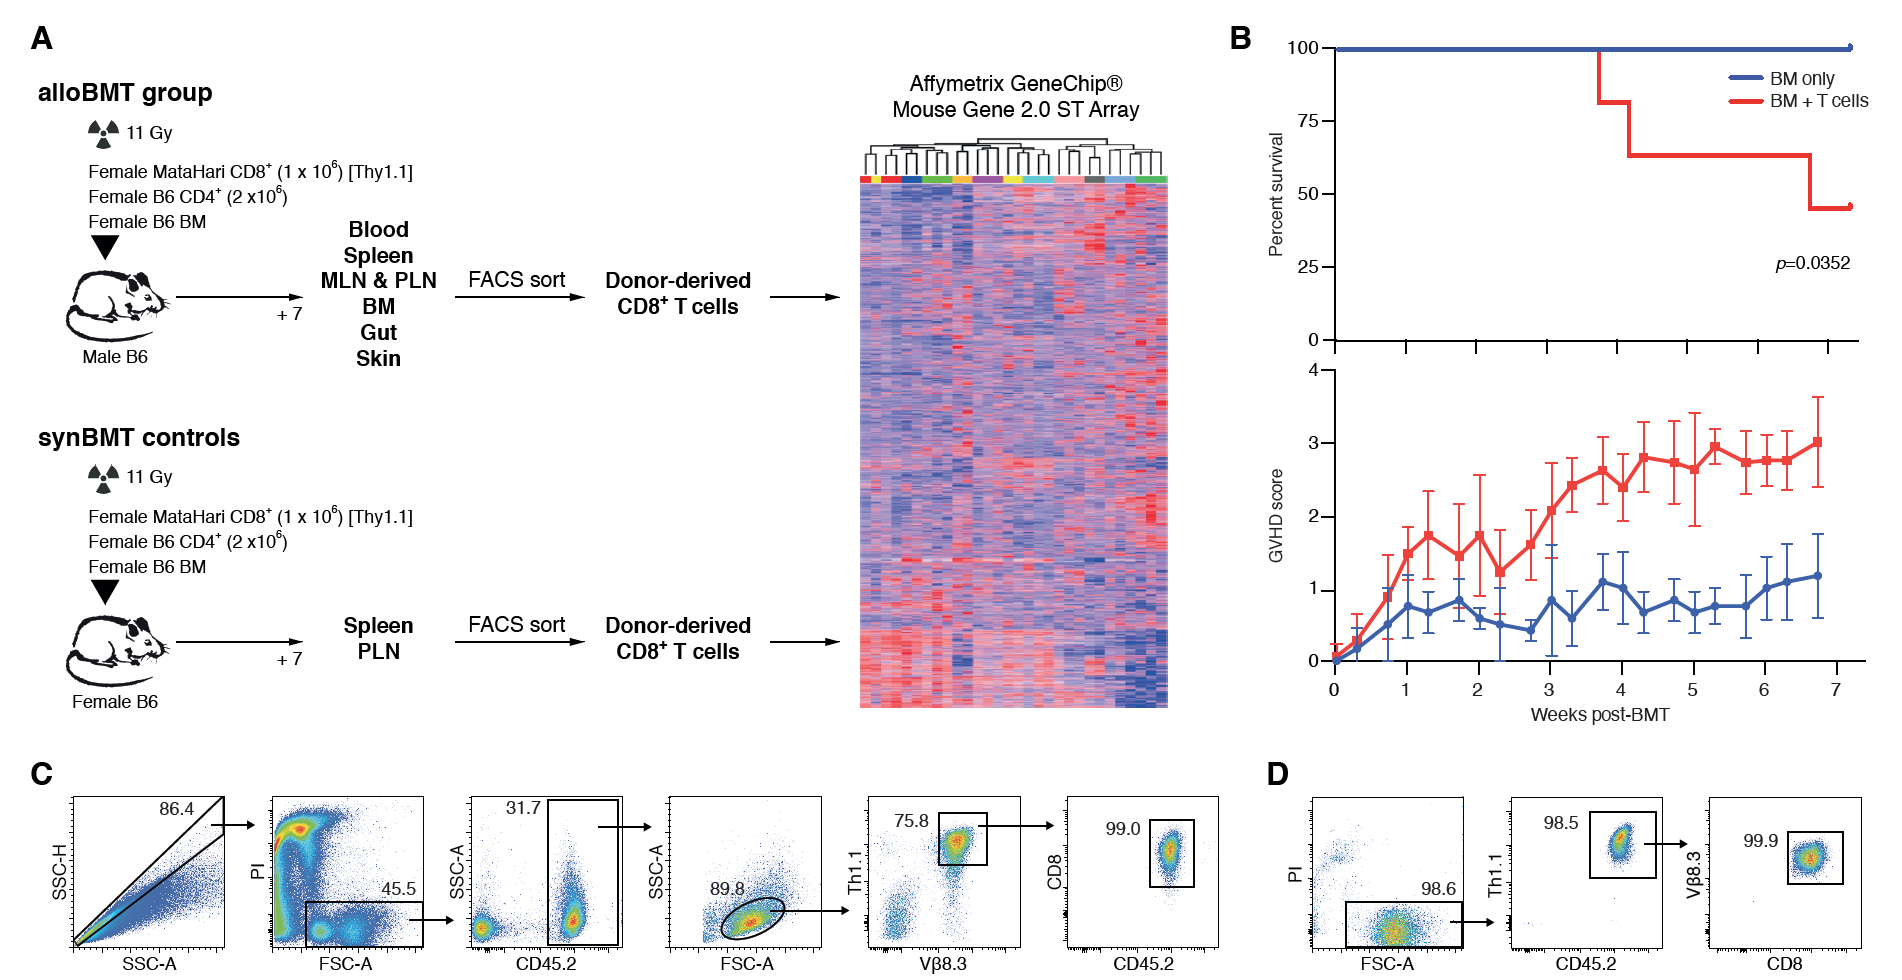
\includegraphics[width=0.9\textwidth]{Figures/Chapter1/MataHari.png}
   \caption{\small{\textbf{(A) Experimental setup.} Female MataHari CD8$\textsuperscript{+}$ T cells were transferred together with female B6 bone marrow and CD4+ T cells into lethally irradiated male B6 recipients (alloBMT group) or female B6 recipients (synBMT controls). Tissue harvesting took place at day +7 post-transplant and donor CD8$\textsuperscript{+}$ T cells were isolated and FACS sorted to high purity. Gene expression profile of sorted cells was assessed by whole-transcriptome microarray analysis. \textbf{(B) Characterization of the GVHD model.} Top graph: Kaplan Meier survival curve (log-rank Mantel-Cox test). Bottom graph: clinical GVHD score over time (mean ± SD). BM only (n=6), BM + T cells (n=11). \textbf{(C) Gating strategy used to sort donor derived CD8$\textsuperscript{+}$ T cells} (exclusion of doublets $\to$ exclusion of propidium iodide positive cells $\to$ exclusion of stroma cells $\to$ morphologic lymphocyte selection $\to$ selection of donor CD8$\textsuperscript{+}$ T cells based on the expression of congenic markers $\to$ confirmation of CD8 positivity). \textbf{(D) Gating strategy to evaluate purity at the end of each sort.} Abbreviations: BM, bone marrow; MLN, mesenteric lymph nodes; PLN, peripheral lymph nodes.} }
    \label{fig:1}
\end{figure}

\subsection{B6 into 129sv model}

\begin{figure}[H] 
    \centering
    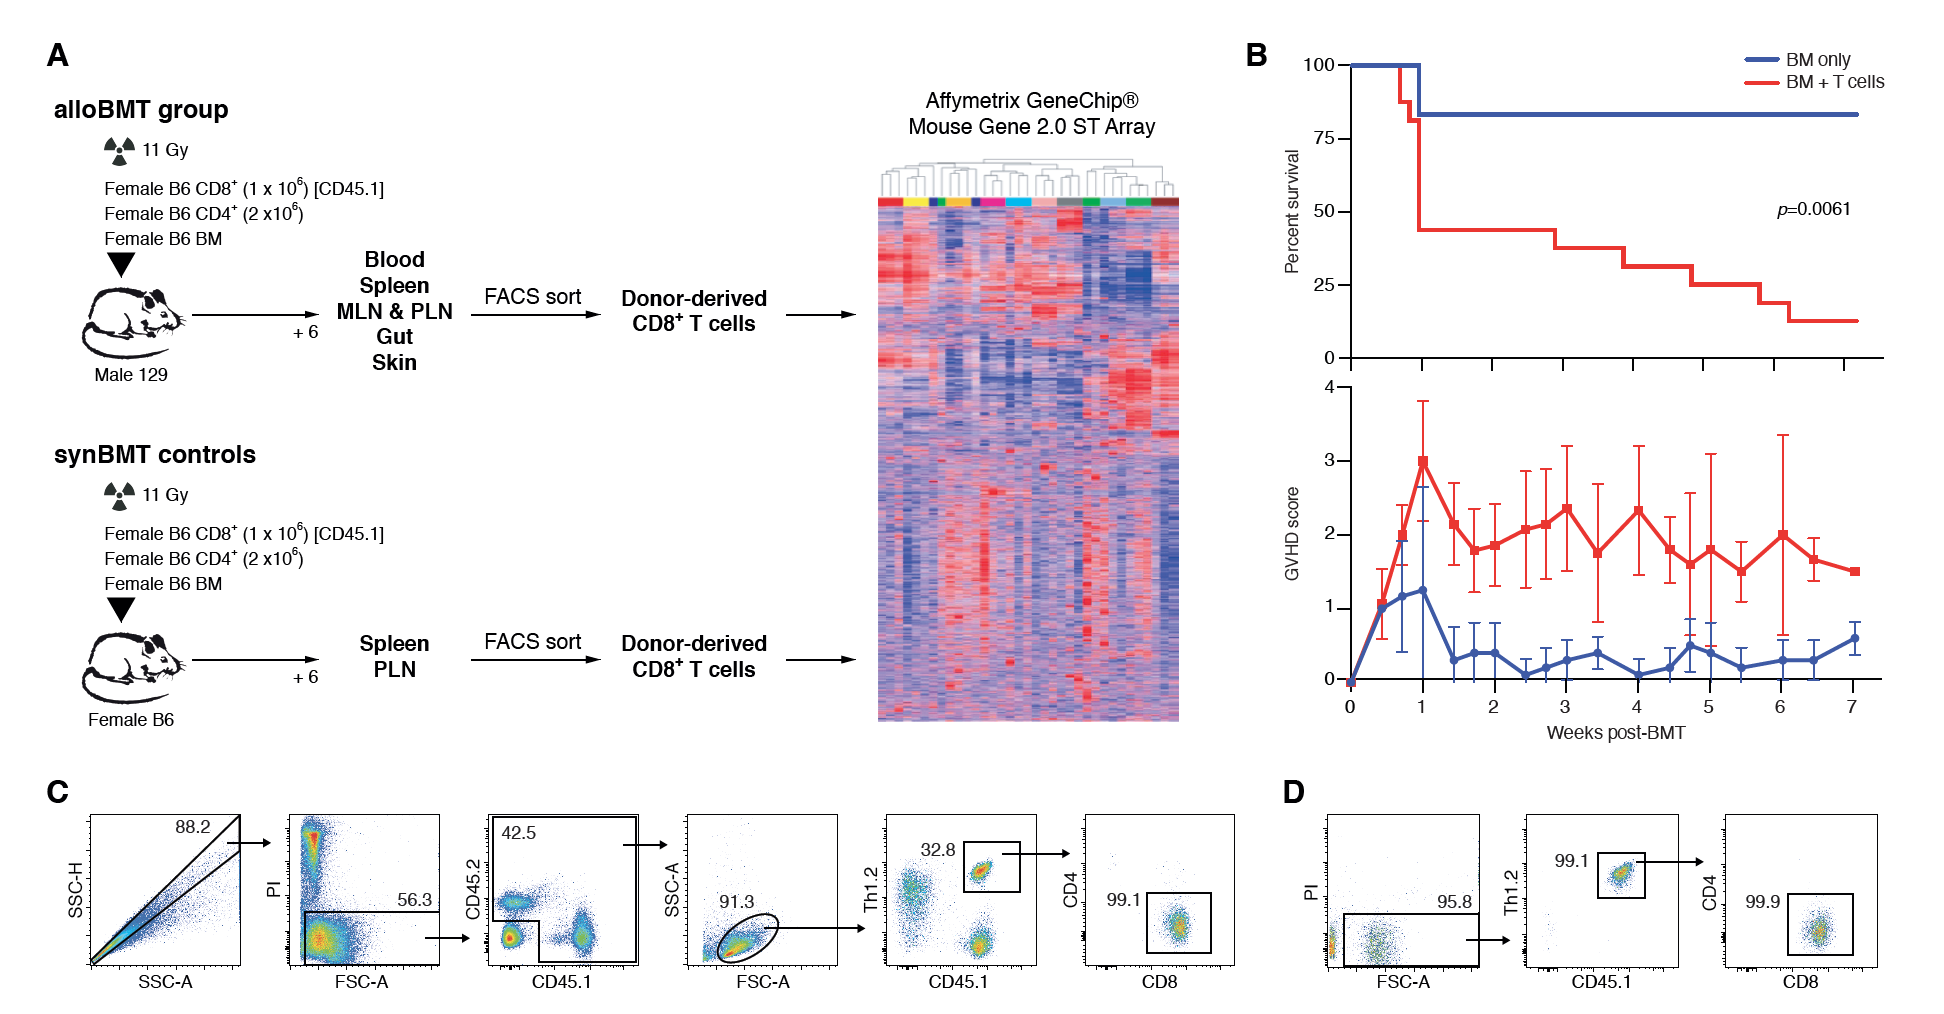
\includegraphics[width=0.9\textwidth]{Figures/Chapter1/B6_129.png}
   \caption{\small{\textbf{(A) Experimental setup.} Female B6 bone marrow and T cells were transferred into lethally irradiated male 129/Sv recipients (alloBMT group) or female B6 recipients (synBMT controls). Tissues were harvested at day +6 post-transplant and donor CD8$\textsuperscript{+}$ T cells were isolated and FACS sorted to high purity. Gene expression profiles of sorted cells was assessed by whole-transcriptome microarray analysis. \textbf{(B) Characterization of the GVHD model.} Top graph: Kaplan Meier survival curve (log-rank Mantel-Cox test). Bottom graph: clinical GVHD score over time (mean ± SD). BM only (n=6), BM + T cells (n=16). \textbf{(C) Gating strategy used to sort donor-derived CD8$\textsuperscript{+}$ T cells} (exclusion of doublets $\to$ exclusion of propidium iodide positive cells $\to$ exclusion of stroma cells $\to$ morphologic lymphocyte selection $\to$ selection of donor CD8$\textsuperscript{+}$ T cells based on the expression of congenic markers $\to$ confirmation of CD8 positivity). \textbf{(D) Gating strategy to evaluate purity at the end of each sort.} Abbreviations: BM, bone marrow; MLN, mesenteric lymph nodes; PLN, peripheral lymph nodes.} }
    \label{fig:2}
\end{figure}


\section{Systems biology approach}

Systems biology is perhaps best described as the adoption of a holistic approach to the task of understanding and interpreting complex biological systems. This field is based upon the premise that the whole is greater than the sum of the parts. In this context, "the whole" is often thought of as the networks that together from the living organism in its entirety. By it very nature this approach requires contribution from many scientific disciplines including biology, physics, computer science and bioinformatics to facilitate the exploration of new dimensions of data space and to tackle ever more challenging biological questions. 

As visualised in Figure 1.3, systems biology is usually thought of as a cyclical concept whereby new biological insights prompt the development of new, more powerful technologies to acquire increasing detailed data, which in turn necessitates the evolution of more advanced computational tools for appropriate analysis of the data obtained. Amongst other achievements, the ability to design predictive, multi-scale models now enables discovery of new biomarkers for disease, drug targeting as well as patient stratification based on unique genetic profiles.

\begin{figure}[H] 
    \centering
   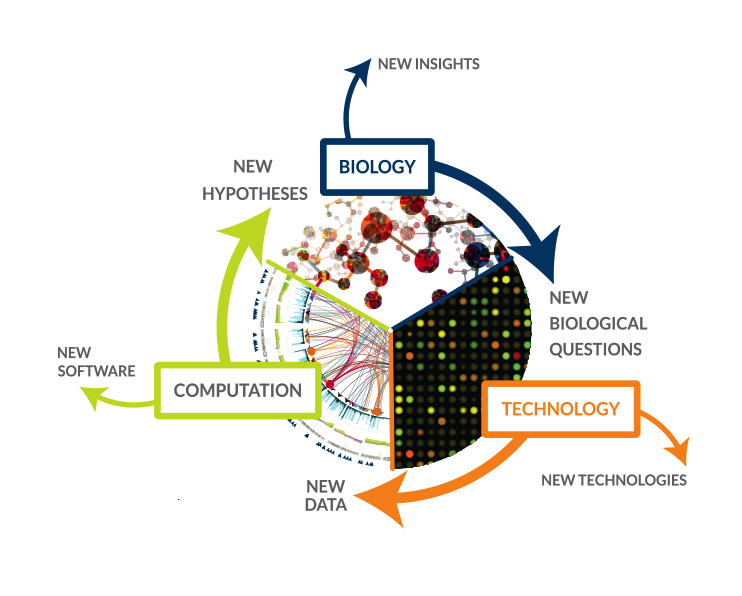
\includegraphics[width=0.8\textwidth]{Figures/Chapter1/systems_bio.jpg}
\caption{\small{The Institute for Systems Biology's depiction of how a cross-disciplinary environment allows for the establishment of a cycle where biology drives technology which in turn drives computation and so on.} }
    \label{fig:3}
\end{figure}

The high-throughput technologies in use today usually generate large lists of hundreds or thousands of potentially biologically interesting genes, but their biological interpretation is still a difficult task ~\autocite{Hua2009}. Indeed, there now exists a plethora of bioinformatics analytical/enrichment tools suitable for use with one or more of the currently available data types. Whilst this has undoubtedly been of huge benefit to thousands of research groups, the amount of choice can leave potential confused and overwhelmed regarding which is the best resource to meet their analytical requirements. It is often advisable for researchers to apply multiple tools from the same branch of analysis type to a given dataset and then manually compare the results and determine which offers the most biologically relevant insights ~\autocite{Hua2009}. In 2009, Huang \textit{et al.} performed a comprehensive analysis of the then available bioinformatics tools ~\autocite{Hua2009}. Although their list is now naturally very outdated, their classification of resources into three groups, namely singular enrichment analysis (SEA); gene set enrichment analysis (GSEA); and modular enrichment analysis (MEA), is still a valid separation. Briefly, SEA involves taking a pre-defined list of interesting genes, e.g. those found to be differentially expressed between case and control with a minimum 1.5 fold change, and linearly testing the enrichment of each known annotation term one-by-one. The major downsides of tools within this set are that the utility of the enrichment is heavily impacted by the quality of the pre-defined gene list and the output is often very large and not user-friendly. GSEA has a similar concept to SEA but with the key difference that GSEA takes as input all genes from a microarray experiment without pre-selection of significant genes. This naturally reduces the likelihood of analytical bias caused by prior determination of which genes are "interesting" and also means that even genes with seemingly small, but nonetheless interesting, changes in expression can still contribute to the analysis. Finally, MEA inherits the basic enrichment calculation found in SEA, but also incorporates network discovery algorithms by considering the term-to-term relationships. When considered together, these inter-relationships between enrichment terms may be of particular interest for the hypothesis under investigation and hence MEA will often produce results that are more easily related back to actual biological interactions than is the case for SEA or GSEA ~\autocite{Hua2009}.

As outlined in a previous section, our laboratory has generated two GVHD datasets using the B6 into 129sv and MataHari mouse models. Given the size and probable complexity of the microarray data obtained, we decided to utilise systems biology techniques to analyse these results and to try to identity clinically relevant gene modules that may help shed some light on the molecular pathways involved in the initiation and progression of GVHD in these mice. 

\subsection{Motivations: Benefit of clustering genes into modules?}

Virtually all cellular functions arise, at least on a fundamental level, as a direct consequence of gene expression patterns and subsequent protein-protein interactions. When considered at a more general level, these interactions can be seen to be organised into molecular pathways and feedback loops which together maintain homoeostatic functionality. Genes and the proteins they encode do not act in isolation but rather as part of one or more pathways or networks and hence it seems appropriate to analyse them in this context. Interconnected genes that form all or part of a biological network where nodes represent genes and edges the interactions between them, are often described as a gene module and it is these entitles that many bioinformatics tools try to identify by clustering together genes exhibiting similar patterns of expression ~\autocite{Lys2011}. These algorithms can be divided into many types based upon the mathematical premises they employ and include topology networks, network clustering, matrix decomposition and heuristic searches ~\autocite{Li2015}.

By attempting to identify gene modules within an expression dataset, we are far more likely to be in a position to understand the molecular implications of the condition/variable we are interested in than if we were to examine single, or even several genes, alone. However, this statement only holds true if the modules we identify and analyse are biologically meaningful and if one considers for a moment the detailed complexity of biological systems on every level, it can be seen that finding such modules is not as straightforward as it may initially appear. 

Many of the clustering algorithms developed to date group genes based on correlation networks between expression profiles as measured by microarray, or similar, techniques. These quantitative analyses typically produce measurements which can be described by an \textit{n} by \textit{m} matrix as follows: 

\begin{equation}
X = |x_ {il}|
\end{equation}

where the row indices correspond to network nodes (\textit{i} = \textit{1, 2,... n}) and the column indices (\textit{l} = \textit{1, 2,.. m}) correspond to sample measurements ~\autocite{Lan2008}. This can be written in the form:

\begin{equation}
\mathbf{X = |x_ {ij}|} = \left(
\begin{array}{c}
x_\textit{1} \\
x_\textit{2} \\
\vdots \\
x_\textit{n}
\end{array} \right)
\end{equation}

We refer to the \textit{i}-th row $x_i$ as the \textit{i}-th node profile across \textit{m} sample measurements. 

The rationale behind correlation network methodology, which is a common analytical choice among biologists, is to use network language to describe the pairwise relationships (correlations) between the rows of X ~\autocite{Lan2008}.

\subsection{How to evaluate quality of clustering results}

With advances in the development of stable gene clustering algorithms, researchers are now faced with questions of how to evaluate the accuracy and validity of modules they identify. However, given the prevalence of such algorithms, there are still surprisingly few established methods for the validation and evaluation of module gene sets. Until fairly recently, aside from size-limited experimental techniques to verify interactions between module members, studies largely relied upon function enrichment tools e.g. Gene Ontology (GO) and KEGG to determine the quality of their modules through enrichment. However, this method rarely produces evenly annotated modules and should theoretically be periodically re-analysed to account for updates made to the annotation database itself ~\autocite{Li2015}. 

In response to these shortcomings, research focus is now shifting to incorporate computational methods into the standard module validation analysis protocols. Such techniques often involve the probing of a modules architectural properties and collectively are sometimes known as Computational Validation Approaches based on Modular Architecture (CVAMA). CVAMA are suitable for application to modules of any size and are not reliant on external databases. In their recent review Li \textit{et al.} divided available CVAMA methods into topology-based approaches (TBA) and statistics-based approaches (SBA) and in the following brief summary we echo their distinctions ~\autocite{Li2015}. 

\subsubsection{topology-based approaches (TBA)}

A gene module can be seen as possessing several network topological features which can be used to quantify its physical parameters. Most analytical projects will tend to focus on one or several of these criteria which are deemed by the researchers to be most relevant for the purpose of establishing whether the proposed modules possess a non-random structure ~\autocite{Don2012}. Here we provide a list of typical parameters examined together with their definitions which have been taken from review of this topic by Doncheva \textit{et al.}~\autocite{Don2012}:

\paragraph{Connected components -} 
When considering an undirected network, any two given nodes are said to be connected if there are one or more edges between them. This parameter provides an indication of global connectivity, with a low value suggesting a strongly connected network.

\paragraph{Degree distributions -} 
For undirected networks, the node degree of a node \textit{n} is the number of edges to which it is linked. The \underline{node degree distribution} gives the number of nodes with degree \textit{k} for \textit{k = 0, 1, etc.} Nodes with high values of \textit{k} are known as hubs. In directed networks, the "in-degree" of node \textit{n} is the number of incoming edges and the "out-degree" is the number of outgoing edges. A network is termed scale-free if its degree distribution approximates a power law $k^{-\alpha}$ with the degree exponent \textalpha. As a general rule for biological studies, hubs with $\alpha >$ 3 are classed as irrelevant, those where 3 $< \alpha >$ 2 tend to possess hierarchical organisation and when $\alpha =$ 2 a 'hub-and-spoke' model (referring to the connectivity of the largest hub) is often seen. In the case of biological networks $\alpha$ is commonly between 2 and 3.

\paragraph{Neighbourhood-related parameters -} 
The set of neighbours for a particular node \textit{n} comprises its neighbourhood. The \underline{connectivity} \textit{kn} is the size of the neighbourhood of \textit{n} and the average of one can give an approximation of the average of the other. A networks density is a normalised version of this parameter. A network without any edges will have a density of 1, while the value for a clique will be 1.

\paragraph{Neighbourhood Connectivity} 

As mentioned above, the \underline{connectivity} of a node \textit{n} is the number of its neighbours. As such the neighbourhood connectivity of node \textit{n} is defined as the average connectivity of all neighbours of \textit{n}. The corresponding \underline{neighbourhood connectivity distribution} summarises the average of the neighbourhood connectivities of all nodes \textit{n} with \textit{k} neighbours for \textit{k = 0, 1, etc.} For directed networks, any given node possess three types of neighbourhood connectivity:

\begin{itemize}
    \item \emph{Only in }- the average out-connectivity of all in-neighbours of \textit{n}
    \item \emph{Only out }- the average in-connectivity of all out-neighbours of \textit{n}
    \item \emph{In and out} - the average connectivity of all neighbours of \textit{n}, where edge direction is ignored
\end{itemize}

Based on these definitions there are three equivalently named neighbourhood connectivity distributions.

\paragraph{Shortest paths -}

The length of a path is represented by the number of edges forming it. The length of the shortest path, or distance, between two nodes \textit{n} and \textit{m} is denoted by L(\textit{n,m}). The \underline{shortest path length distribution} gives the number of node pairs (\textit{n,m}) with L(\textit{n,m}) = \textit{k} for \textit{k = 0, 1, etc.} The \underline{eccentricity} of a node \textit{n} is the maximum non-infinite length of a shortest path between \textit{n} and another node in the network. The \underline{network diameter} is the maximum node eccentricity. 

the \underline{network radius} is defined as the minimum of the nonzero eccentricities of the nodes in the network. The \underline{average shortest path length} gives the expected distance between two connected nodes.

\paragraph{clustering coefficients -}

In undirected networks, the clustering coefficient $C_n$ of a node \textit{n} is defined as $C_n = 2e_n/(k_n(k_n–1))$, where $k_n$ is the number of neighbours of \textit{n} and $e_n$ denotes the number of edges between all neighbours of \textit{n}. In directed networks, this coefficient is parametrised by $C_n = e_n/(k_n(k_n–1))$. 

In both instances, the clustering coefficient is a ratio \textit{N/M}, where \textit{N} is the number of edges between the neighbours of \textit{n}, and \textit{M} the maximum number of edges that could possibly exist between the neighbours of \textit{n}. For any given node \textit{n}, this value is always between 0 and 1. 

The \underline{network clustering coefficient} is the average of the clustering coefficients of all nodes in the network and the \underline{average clustering coefficient distribution} gives the average of the clustering coefficients for all nodes \textit{n} with k neighbours for \textit{k = 2, 3, etc}.  

\paragraph{Shared neighbours -}

Defined as \textit{P}(\textit{n,m}), this parameter represents the number of interaction partners shared between nodes \textit{n} and \textit{m}. The \underline{shared neighbours distribution} gives the number of node pairs (\textit{n,m}) with \textit{P}(\textit{n,m}) = \textit{k} for \textit{k = 1, 2, etc}. 

\paragraph{Topological coefficients -}

The topological coefficient $\textit{T}_n$ of a node \textit{n} with $\textit{k}_n$ neighbours is computed as: 

\begin{equation}
\textit{k}_n = avg (\textit{J}(\textit{n, m}))/\textit{k}_n
\end{equation}

Here \textit{J}(\textit{n, m}) is defined for all nodes \textit{m} that share at least one neighbour with \textit{n}. 
The value \textit{J}(\textit{n, m}) is the number of neighbours shared between the nodes \textit{n} and \textit{m}, plus 1 if there is an edge between \textit{n} and \textit{m}. This coefficient is a relative measure for the extent to which a given node \textit{n} shares neighbours with other nodes. 

\paragraph{Stress centrality -}

The stress centrality of a given node \textit{n} is the number of shortest paths passing through \textit{n}. The \underline{stress centrality distribution} gives the number of nodes with stress \textit{s} for \textit{s = 1, 2, etc}. 

\paragraph{Betweenness centrality -}

The betweenness centrality $C_b\textit{(n)}$ of a node \textit{n} is defined as:

\begin{equation}
C_b\textit{(n)} = \textstyle \sum_{s\neq n\neq t}^{}  (\sigma_{st}(n)/\sigma_{st})
\end{equation}

where, \textit{s} and \textit{t} are nodes in the network other than \textit{n}, $\sigma_{st}$ gives the number of shortest paths from \textit{s} to \textit{t}, and $\sigma_{st}(n)$ is the number of shortest paths from \textit{s} to \textit{t} that pass through \textit{n}.

This parameter is only computed when a network is comprised of single edges alone. 

The betweenness value for each node \textit{n} is normalised to lie between 0 and 1 by dividing the number of node pairs excluding \textit{n} as follows:
\begin{equation}
(\textit{N} -– 1)(\textit{N} -– 2) / 2
\end{equation}
 where \textit{N} is the total number of nodes in the connected component that \textit{n} belongs to. The betweenness centrality of a node reflects the amount of control it exerts over the interactions of other nodes in the network.

\paragraph{Closeness centrality -}

The closeness centrality $C_\textit{(n)}$ of a node n is the reciprocal of the average shortest path length. The closeness centrality of each node \textit{n} is a value between 0 and 1 and is a measure of how quickly information spreads from a given node \textit{n} to other reachable nodes in the network.

Several topological indexes have also been developed to evaluate a given module's likely validity. These include the the network perplexity index of Entropy where a good quality module is expected to have a low entropy ~\autocite{Zha2009}. This index is typically defined as follows: 

\begin{equation}
Entropy (M) = -\textstyle \sum_{J \in {bins}}^{} P_j log_2 P_j
\end{equation}

Another widely used single index is the NB Value which is used to identify modules with high intra-modular connectivity (NB $\geq$ 0.5) ~\autocite{Oza2010}. The NB Value represents a ratio of edges within a module and the total number of edges between modules:

\begin{equation}
NB = \frac{\sum e(i)} {\sum d(i)} 
\end{equation}

To be of informative value it is vital that the index chosen to validate a module should be independent of the methods used to identify the module. It is also common practice for multiple topological indexes or module preservation statistics to be combined into an integrated measure for the overall assessment of module validity or preservation. Perhaps the most widespread composite preservation statistic used to validate whether a module is significantly preserved in another network is the Z\textsubscript{summary} score ~\autocite{Lan2011}: 

\begin{equation}
Z_{summary} = \frac{Z_{density} + Z_{connectivity}} {2} 
\end{equation}

A Z\textsubscript{summary} score of $\geq$ 10 indicates that a module is strongly preserved, a value between 2 and 10 suggests moderate preservation and if this index produces a score $\leq$ 2 then no preservation is found. 

\subsubsection{statistics-based approaches (SBA)}

As well as exhibiting some form of modular structure which can be analysed using the topological criteria detailed above, a "good" gene module should be statistically significant i.e. its architecture distribution ought to be very unlikely to be obtained by chance in a randomised network. It is often also important to quantify relationships between modules and phenotypic characteristics and this too requires some measurement of statistical significance. Depending on the biological context it is possible to use binary or mixed integer linear models to validate causal or dependent relationships between network modules and biological phenotypes ~\autocite{Hen2011,Sch2011,Shi2010}. Using a permutation test with a \textit{p}-value calculated by estimating the null distribution we are able to determine whether the composition of a given module is higher than expected by chance or is associated with a particular disease phenotype ~\autocite{Jia2012}. As mentioned above, comparative network analysis techniques such as Z\textsubscript{summary} can also aid the identification of conserved modules across networks or species, as well as providing insight into the reproducibility of the module in question. 


\subsection{Two complementary approaches to module definition}

\subsection{Prior generation of MataHari modules using WGCNA}

To tackle the hypothesis mentioned previously, i.e. to measure the respective roles of lymphoid organs and peripheral tissues in dictating T cell effector programs that result in tissue injury, our team began by characterising the transcriptional response of donor CD8$\textsuperscript{+}$ effector T cells as they trafficked to multiple sites during the evolution of GVHD. This enabled the analysis of how T cells differentiate within secondary lymphoid organs (SLO) compared to those in peripheral tissues. Experiments using the MataHari and B6 into 129sv GVHD models were performed as outlined in Figures 1.1 and 1.2 respectively. Once microarray data had been acquired from the B6 into 129sv experiments, skin- and gut-tissue specific genes, determined using PaGenBase, were removed from the datasets to correct for any contamination by other celltypes. Multi-dimensional scaling (MDS) was performed on both datasets and as evidenced by Figure 1.4A, not only do allogeneic recipients segregate separately from both na\"ïve T cells and those undergoing proliferation within lymphatic tissues, but there is also a clear distinction within recipients of allogeneic BMT between those T cells deriving from secondary lymphoid organs (plotted as blue circles) and those within GVHD target tissues (shown as red circles in the plot). 

\begin{figure}[H] 
    \centering
   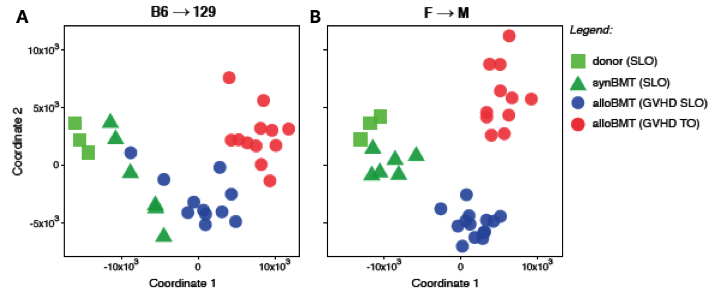
\includegraphics[width=0.8\textwidth]{Figures/Chapter1/lab_MDS_plot.png}
\caption{\small{Multi-dimensional scaling (MDS) plots depicting the proximity of the transcriptional profiles of donor derived CD8$\textsuperscript{+}$ T cells isolated from the spleen, lymph nodes, blood, gut and skin, in the two model systems (B6 into 129sv and MataHari Female $\to$ Male).} }
    \label{fig:4}
\end{figure}

It was concluded that these observed differences in gene expression profiles could be the result of either tissue environment-dependent re-programming or the selection of pre-existing variants from the bulk population. To exclude the latter option the experiments were repeated in the MataHari B6 female $\to$ B6 male. This BMT model involves the transfer of na\"ive MataHari CD8$\textsuperscript{+}$ T cells transgenic for a TCR that recognises a single, ubiquitous HY antigen, Db-Uty. As can be seen in Figure 1.4B, the expression profiles of T cells found in GVHD target organs are again clustered away from those in the secondary lymphoid organs. Additionally, there was a substantial amount of overlap identified between effector T cell expression profiles from each tissue in the MataHari Female $\to$ Male dataset and the equivalent sample in the B6 into 129sv model which supports the theory that differences in effector T cell profiles reflected the source tissue and were independent of the T cell receptor repertoire. Given the profound separation seen between tissue groups in the MataHari Female $\to$ Male model, this dataset was taken forward for further analysis. 

Using the analytical method Weighted Gene Correlation Network Analysis (WGCNA), which is detailed in Chapter \ref{Chapter3}, modules of co-expressed genes were identified within the Female $\to$ Male data in the hope that they may assist in gaining an understanding how tissue specific effector T cell transcriptional programs develop. A total of 31 such gene modules were found and the inter-module expression patterns were seen to vary substantially between both the type of BMT (syngeneic or allogeneic) and the tissue source of the T cells. This diversity in module expression profiles, which is portrayed in Figure 1.5A, even extended to tissue sub-compartments (e.g. the dermis versus the epidermis). As evidenced by this Figure, a marked distinction was observed between those modules up-regulated in GVHD target organs compared to the secondary lymphoid organs which is of great interest given our hypothesis of tissue specific re-programming of effector T cells. In order to determine how well these 31 modules were conserved in the B6 into 129sv model the Z\textsubscript{sum} composite preservation measurement was used. Of the 31 modules identified in the Female $\to$ Male dataset 30 were found to be conserved in the B6 into 129sv dataset based on a Z\textsubscript{sum} > 2.0, while 19 modules passed the cut-off at Z\textsubscript{sum} > 10. These 19 modules were subsequently annotated to identify enriched biological processes using the Gene Ontology database ~\autocite{Ash2000,GO2015} and candidate driver genes i.e. genes exhibiting high intra-modular connectivity were pinpointed. The most significant biological process annotations and likely driver genes are shown in Figure 1.5B. 

\begin{figure}[H] 
    \centering
   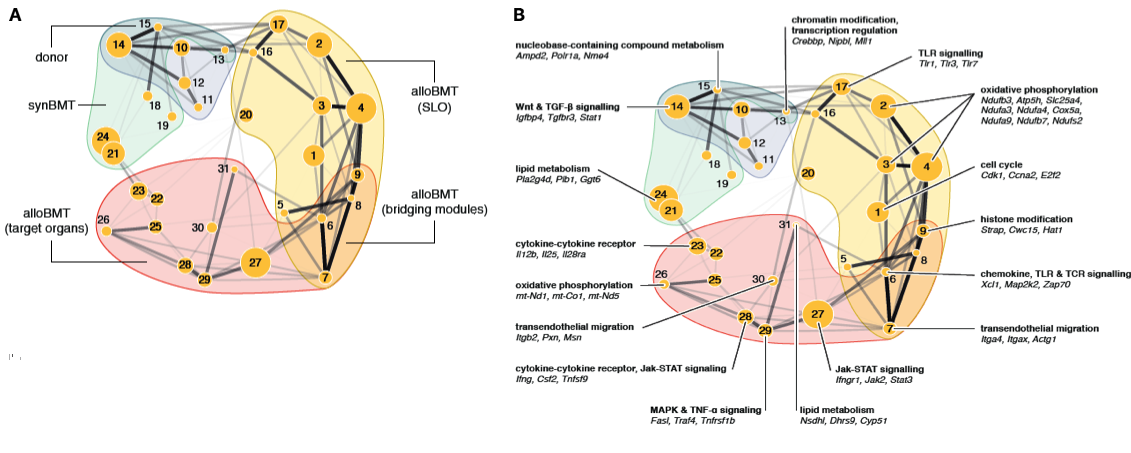
\includegraphics[width=0.9\textwidth]{Figures/Chapter1/MH_mods.png}
\caption{\small{A. Summary Eigengene network where shaded areas represent MataHari Female $\to$ Male module clusters associated with the surveyed experimental groups and GVHD subgroups. B. MataHari Female $\to$ Male modules classified according to the main classes of Gene Ontology terms of the annotated genes. Putative driver genes for each conserved module were identified on the basis of high intra-modular connectivity (3 examples per module).} }
    \label{fig:5}
\end{figure}

Further details and discussions of these findings will not be included here but given the importance of this dataset for work presented later in this report, the following represents a summary of the authors primary observations: 

\begin{enumerate}
    \item Several, strongly interconnected gene clusters segregated primarily with the SLO origin of effector T cells e.g. M17 was strongly correlated with T cells from the LN but negatively correlated with those of GVHD target organs; 
    \item M1 which contains genes associated with DNA replication and the cell cycle mapped to blood and BM-derived effector T cells;
    \item M3 segregated with the spleen and BM TE and was almost exclusively comprised of fatty acid oxidation and oxidative phosphorylation related genes;
    \item M7 which contained genes encoding proteins implicated in cytoskeletal reorganisation and transendothelial migration was the most densely interconnected of the bridging modules;
    \item  The largest GVHD target organ-specific module was M27. This module was enriched for multiple intracellular signalling gene pathways including MAPK and JAK-STAT;
    \item M28 was highly specific for effector T cells of the epidermis and contained a strong Ifng-related signal with genes for multiple pro-inflammatory cytokines, cytokine receptors and downstream adaptors;
    \item  M29 segregated with the majority of GVHD target organs and is considered by the authors to represent a pan-GVHD target organ gene cluster;
    \item  Driver genes identified within the M7, M28 and M29 modules, showed a high degree of overlap with a Th1/17-related pathogenicity gene cluster that is linked to aggressive T cell autoimmunity
\end{enumerate}
 
It can thus be seen that this MataHari dataset together with the WGCNA-derived gene modules discussed briefly above represent a highly useful and detailed resource from which we can potentially learn much regarding the impact of tissue specific effector T cell imprinting on GVHD pathology. 
 


\chapter{Current knowledge of T cell transcriptional profiles} % Main chapter title

\label{Chapter2} % For referencing the chapter elsewhere, use \ref{Chapter1} 

%----------------------------------------------------------------------------------------

%----------------------------------------------------------------------------------------
\section{Overview}

In this Chapter we review current knowledge of how CD4$\textsuperscript{+}$ and CD8$\textsuperscript{+}$ T cells differentiate, together with an examination of the characteristic features of the resulting populations. We also discuss details of T cell activation in response to antigen presentation and how gaining a full understanding of these mechanisms is relevant to GVHD research. 

\section{Differentiation of T cell subtypes}

CD4$\textsuperscript{+}$ T helper and CD8$\textsuperscript{+}$ cytotoxic T cells are required for the generation of powerful and specific responses of the host when faced with pathogenic challenges ~\autocite{Won2016}. Both of these cell lineages develop from multipotent progenitors in the bone marrow or fetal liver. These progenitor populations subsequently go on to seed the thymus by a process of continuous migration. As precursors of the $\gamma \delta$ lineage enter the thymus, significant changes in their expression patterns of class I homeobox (HOX) genes are seen. This highly conserved family of transcription factors are indispensable for the appropriate regulation of embryogenesis and there is evidence to suggest that they may also influence T cell developmental pathways ~\autocite{Tag2003}. At the initial stage of development these T cells, known as thymocytes, are referred to as double negative (DN) by virtue of the fact that they do not express either CD4 or CD8 on their surface ~\autocite{Wee2006}. For murine lymphocytes this DN population is subdivided into three classes of maturity based upon T cell receptor expression patterns. The first group are called DN1 cells and possess the signature of CD117$\textsuperscript{+}$CD44$\textsuperscript{+}$CD25$\textsuperscript{-}$. It is noteworthy that in humans, cells at this highly immature phase of differentiation are characterised as CD34$\textsuperscript{+}$CD1a$\textsuperscript{-}$CD38$\textsuperscript{-}$ and are homologous to the DN1 cells of mice. Following some minor T cell receptor gene rearrangement, DN2 cells are formed which express CD117$\textsuperscript{+}$CD44$\textsuperscript{+}$CD25$\textsuperscript{+}$. Next, T cells characterised by CD117$\textsuperscript{-}$CD44$\textsuperscript{-}$CD25$\textsuperscript{+}$ expression are produced by major T cell receptor gene rearrangement ~\autocite{Koya2012}. These DN3 cells are further classified into two sub-populations which are referred to as DN3a and DN3b before and after $\beta$ selection respectively ~\autocite{Koya2012}. Indeed, it is the expression of T cell receptor $\beta$ that now qualifies the cells to undergo $\beta$-selection. It is at this point that cells become fully committed to the T cell lineage and begin to express CD4 and CD8 to become double-positive (DP) cells ~\autocite{Koya2012}. Interestingly Taghon \textit{et al.} observed the systematic, genomic position based down-regulation of HOX-A genes as thymic T cells increased in maturity, indicating that these transcription factors may have undetermined impacts on the differentiation of T cells subsets ~\autocite{Tag2003}. In the final stages of T cell differentiation in the thymus, triple-negative CD117$\textsuperscript{-}$CD44$\textsuperscript{-}$CD25$\textsuperscript{-}$ DN4 cells are generated which can then undergo positive and negative selection to generate mature CD4$\textsuperscript{+}$ or CD8$\textsuperscript{+}$ single-positive (SP) T cells that migrate to the periphery ~\autocite{Wee2006,Won2016,Koya2012}. This trafficking, or homing, of primed T cells primed i.e. those cells that have been activated by the primary recognition of specific peptide–MHC complexes, is required to ensure a directed, localised immune response and is primarily under the control of tissue-selective chemokines and their receptors ~\autocite{Gri2014}. The expression of adhesion molecules on the surface of migratory T cells and recognition of antigen expressed by endothelial cells also aid homing to sites of inflammation by facilitating interactions with membrane-bound integrins ~\autocite{Fu2013}. The collective expression of chemokines and adhesion molecules is sometimes used to determine the functional abilities and activation status of T cell populations ~\autocite{Won2016}. 

T cell malignancies are still prevalent worldwide and can develop at any stage of the differentiation process as well as from mature T lymphocytes in the peripheral circulation ~\autocite{Fil2002}. T-cell acute lymphoblastic leukaemia (T-ALL) for example is characterised by the abnormal proliferation of immature pre-T cell clones together with abnormal hematopoiesis and is often fatal due to the accumulation of organ infiltrates or infection ~\autocite{Tia2013}. Whilst dysfunctional T cells are a feature of T-ALL, it is currently unclear how this disease is initiated and progresses. Indeed, unlike B-cell lymphomas chromosomal translocations are only seen in a small percentage of peripheral T-cell lymphomas ~\autocite{Fil2002}. Thus, while we may possess a broad understanding of the steps involved in T cell differentiation in the thymus, there is great incentive to tackle the many questions that remain. These include, for example, quantifying the importance of Notch signalling during T cell differentiation. Notch signalling, or to give the full title the Notch signal transduction pathway, comprises a collection of highly conserved transmembrane receptors and their ligands which together influence multiple developmental processes. There are four receptors within this family, called Notch 1 to 4, which signal via the binding of a ligand on a nearby cell to the extracellular domain of the receptor protein. In mammals Jagged 1 and 2 together with Delta 1, 3 and 4 represent the known Notch ligands. This receptor-ligand interaction causes proteolytic cleavage of the Notch receptors' intracellular domain which is then free to translocate to the nucleus where it binds the transcription factor CSL and activates transcription of target genes including Hairy-Enhancer of Split (HES)1 and HES5 and Hes-related repressor protein (HERP) ~\autocite{Wee2006}. Initially, a role for Notch 1 in T cell differentiation was proposed following studies of mice with a conditional deletion of this gene in which T cell development was completely halted at the DN1 stage ~\autocite{Wee2006,Koya2012}. Notch has also been shown to be required for successful $\beta$ selection in the thymus. Furthermore, over-expression of this protein within the bone marrow was shown to induce T cell differentiation at the expense of B cell development. The involvement of Notch signalling in these cell developmental pathways is very much in keeping with the known functions of these proteins which often form part of cell-fate determining processes ~\autocite{Koya2012}. It is interesting to ponder then why other members of the Notch receptor family do not seem to play a role in the regulation of T cell development. Koyanagi \textit{et al.} obtained data suggesting that Notch 2 and 3 were expressed on the same DN thymocyte population as Notch 1 and yet their presence seems to have no direct effect ~\autocite{Koya2012}. As postulated by the authors, this finding may be the result of a differential glycosylation modification of Notch receptors by Fringe proteins ~\autocite{Koya2012,Leb2014}.

As summarised in Figure 2.1, na\"ive CD4$\textsuperscript{+}$ cells, once activated by interactions with APCs, will differentiate into one of four specialised celltypes, defined by distinct cytokine secretion, trafficking receptor expression, and the presence of a master transcriptional regulator ~\autocite{Zhu2010}, which all have critical roles in adaptive immune responses. The activation of T cells will be covered in depth elsewhere, suffice to say that the initiation of T cell differentiation requires the recognition of an MHC class II/cognate antigen complex on the surface of an APC ~\autocite{Edw2014}. Putting aside the Treg population which will be discussed later, it was originally thought that there were only two possible fates for CD4$\textsuperscript{+}$ cells, namely the Th1 and Th2 lineages ~\autocite{Awa2009}. This conclusion was based upon observations that Th1 and Th2 cells produce differing patterns of cytokines and possess distinct functions. While Th1 lymphocytes are necessary for the cell-mediated immunity against intracellular pathogens and secrete interferon-$\gamma$, lymphotoxin and IL-2, Th2 cells produce IL-4,IL-5 and IL-13 and are responsible for clearing pathogens and extracellular parasites ~\autocite{Mil2010,Awa2009, Cha2003}. Recent research has in fact challenged this classification with claims that it is too simplistic to explain the complexity of the events that lead to pathogen clearance and immune tolerance ~\autocite{Mil2010}. Indeed, there is now a great deal of evidence to support support the existence of another CD4$\textsuperscript{+}$ IL-17 secreting sub-population with unique effector function termed Th17 cells which are believed to differentiate following release of IL-23~\autocite{Awa2009}. Studies in mouse models suggest that Th17 cells are involved in defence against extracellular pathogens and that they may be implicated in inflammatory autoimmune conditions ~\autocite{Cro2009}. 

\begin{figure}[H] 
    \centering
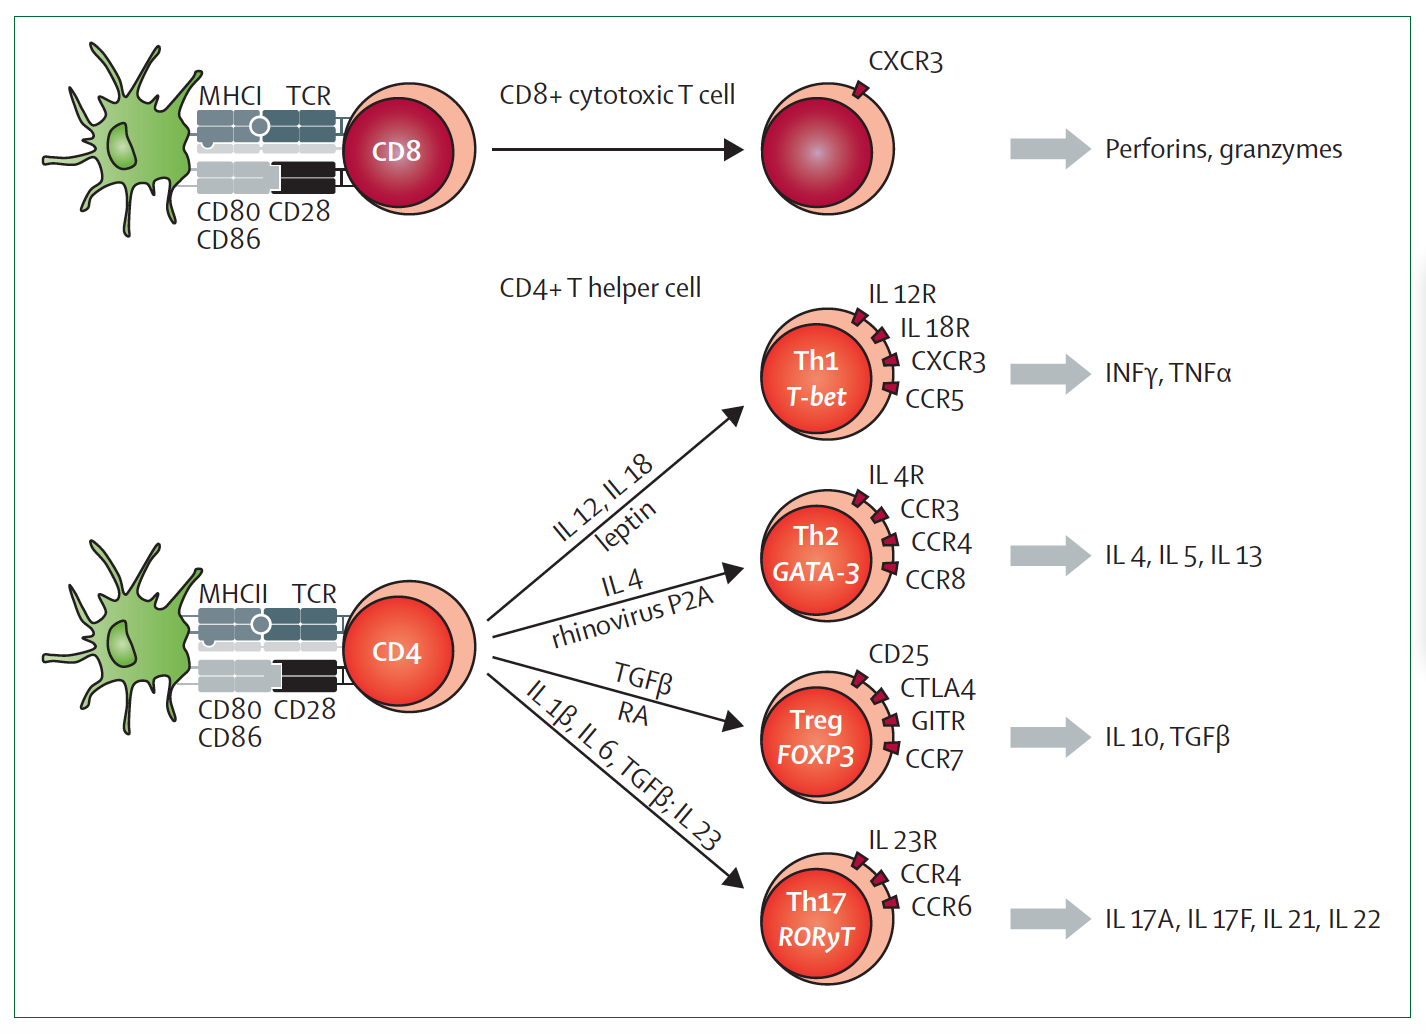
\includegraphics[width=0.8\textwidth]{Figures/Chapter2/T_cell_differentiation.png}
\caption{\small{Outline of CD4$\textsuperscript{+}$ and CD8$\textsuperscript{+}$ T cell differentiation in response to stimulation by antigen. Taken from Brusselle \textit{et al.}, 2011 ~\autocite{Bru2011}.} }
    \label{fig:6}
\end{figure}

As alluded to briefly above, it is the antigen specific activation of the T cell receptor in the presence of a polarising cytokine milieu that triggers the differentiation of T cells into a specific Th subset ~\autocite{Cha2003}. The particular lineage a cell will be committed to is additionally influenced by the concentration of antigen, strength of the TCR signal, ligation of co-stimulatory molecules, current chromatin structure and the type of APC involved in the interaction ~\autocite{Cha2003,Edw2014}. It is known that, upon antigen driven TCR stimulation, the production of Th1 cells occurs in response to the activation of Signal Transducer and Activator of Transcription (STAT)-1 and STAT-4 by IL-12 and interferon-$\gamma$ which in turn upregulate a Th1-specific transcription factor known as T-bet ~\autocite{Awa2009, Edw2014}. T-bet acts as a major player in the initiation of interferon-$\gamma$ production and hence a positive feedback loop is initiated ~\autocite{Edw2014,Tia2013}. The likely accuracy of these assertions is suggested by the observation that a deficiency in T-bet causes partial inhibition of interferon-$\gamma$ release and prevents Th1 differentiation ~\autocite{Edw2014}. Th1 cells are required for cell-mediated immune defense against intracellular pathogens and are implicated in multiple autoimmune pathologies ~\autocite{Cha2003}. These cells are also involved in the activation of CD8$\textsuperscript{+}$ CTLs and their frequency is found to be decreased in T-ALL ~\autocite{Tia2013}. It is believed that T-bet is able to influence epigenetic states of T-helper cells due to its ability to control the state of the H3K27me3 modification. This property of T-bet allows for some flexibility of the signature gene expression program of Th cells until it is extinguished ~\autocite{Mil2010}. Thus it is possible that the re-expression of this transcription factor in newly differentiated T helper cells may significantly alter their fate and effector properties. 

In contrast to the Th1 population, STAT-6 together with the transcription factor GATA-binding protein 3 (GATA-3) controls the differentiation of Th2 cells. IL-4 is the main cytokine produced by the Th2 population but the release of  IL-5, IL-6, IL-9, IL-10 and IL-13 by these cells has also been recorded ~\autocite{Cha2003}. The distinctions between the development of Th1 and Th2 lineages are highlighted by the fact that T-bet acts to repress expression of GATA-3, thus preventing differentiation of the Th2 lineage ~\autocite{Cha2003,Edw2014}. Chakir \textit{et al.} were among the first to propose that, in a population of mixed cells, the Th1 and Th2 cytokine expression patterns are best described by the T-bet/GATA-3 ratio, as against expression levels of either alone, and that GATA-3 is the more potent regulator ~\autocite{Cha2003}. It was in fact analyses of these transcription factors and STAT proteins that lead to identification of IL-17 cells as a distinct lineage as none associated with Th1 or Th2 lineages were found to be expressed by this population. Instead, human IL-17 cells are known to secrete IL-17A, TNF-$\alpha$, IL-6, CD161, IL-22 and IL-26 but are incapable of producing interferon-$\gamma$ ~\autocite{Cro2009}. Even more convincingly, TGF-$\beta$, which along with IL-6, IL-21 and IL-23 is important for the specialisation of TH17 cells \textit{in vivo} via induction of phospho-STAT3, actually inhibits T-bet and GATA-3, thereby preventing differentiation of both Th1 and Th2 populations ~\autocite{Awa2009,Sch2014}. Another feature which sets Th17 cells apart from Th1 and Th2 populations is a lack of self-amplification abilities. Th1 cells are amplified by a positive feedback loop involving IFN-c, STAT-1 and T-bet, while IL-4 fulfils a similar role in in the case of Th2 cells. IL-17 on the other hand is not a differentiation factor and its receptor is not expressed on T cells ~\autocite{Awa2009}. There was some discussion of whether IL-23 might be the primary differentiation factor for Th-17 cells but this was later dismissed due to incompatible expression patterns and a lack of experimental evidence and so debate continues over the precise cytokine activity that optimally induces the development of Th-17 cells ~\autocite{Cro2009}. TGF-$\beta$ and IL-6 have been demonstrated as helping to polarise na\"ive CD4$\textsuperscript{+}$ T cells into Th17 cells in mice, while IL-23 is thought to be required for the expansion, maintenance and effector function of this population ~\autocite{Cro2009, Awa2009, Sch2014}. Although some early studies suggested that TGF-$\beta$ actually had an inhibitory function on Th17 cell differentiation, later work produced countering results ~\autocite{Awa2009}. The requirement for TGF-$\beta$ in the successful differentiation of Th17 cells is therefore still debated, as is the cellular source of this factor which can be produced by multiple leukocyte lineages. What is known is that the successful differentiation of Th17 cells requires the actions of multiple transcription factors. As well as STAT-3 which has already been mentioned, Ror-$\gamma$ t, Ror-$\alpha$ and interferon-regulatory factor 4 all play a part ~\autocite{Cro2009}. Once fully specialised, it is the production of the inflammatory cytokine IL-17 itself that is believed to be crucial for many effector functions of Th17 cells including maintaining mucosal barriers and the efficient clearance of pathogens/fungal infections ~\autocite{Cro2009,Gau2015}. In addition, IL-17 is responsible for the stimulation of cytokine and chemokine release from numerous celltypes and can also assist in the recruitment of neutropils to sites of inflammation. Dysregulation of Th17 effector response can cause dangerous levels of tissue inflammation in the host ~\autocite{Awa2009}. Interestingly, Wong \textit{et al.} comment that in their recent analysis they identified Th cells capable of secreting multiple Th cell-associated cytokines, e.g. cells producing  IFN-$\gamma$, IL-17, and IL-22 simultaneously ~\autocite{Won2016}. 

Regulatory T cells (Tregs), usually subdivided into natural Tregs (nTregs) and adaptive or induced Tregs (iTregs), are circulating CD4$\textsuperscript{+}$ cells well known as being able to suppress both physiological and pathological immune responses. Indeed, a deficiency of Tregs leads to serious systemic autoimmunity ~\autocite{Sch2014}. Focusing on involvement with malignant tumours, it has been seen that Tregs localise to the vicinity of the the damaged tissue which they may be attracted to by chemokine release from the tumour itself. For example, some tumours secrete the chemokine (C-C motif) ligand 22 (CCL22) which is recognised by the chemokine (C-C motif) receptor 4 (CCR4), that is expressed on the surfaces of Tregs in high concentrations ~\autocite{Sch2014}. Tregs are selected in the thymus based on high-avidity interactions and nTregs comprise between 5 and 10\% of total CD4$\textsuperscript{+}$ cell counts ~\autocite{Sch2014}. These cells are characterised by their expression of forkhead box P3 TF (Foxp3). There is evidence that TGF-$\beta$ is important for the differentiation of Foxp3$\textsuperscript{+}$ nTreg cells from naive CD4$\textsuperscript{+}$ T cells as well as maintenance of their functional capabilities ~\autocite{Awa2009}. It has been proposed that nTregs are formed in the thymus in a two-step process. Initially Treg precursors are generated which requires factors such as CD-28 and various cytokine receptors and this is then followed by the binding of IL-2 to its receptor and the resulting expression of Foxp3 ~\autocite{Sch2014}. It is interesting to note that low concentrations of TGF-$\beta$ promote Foxp3 expression, thereby favouring Treg differentiation, while at high levels TGF-$\beta$ induced upregulation of the IL-23 receptor leads to the IL-17 phenotype ~\autocite{Sch2014}. IL-2 has also been shown to activate the tumour effects of NK cells ~\autocite{Tia2013}. The fact that Th17 and Treg cells undergo mutually exclusive differentiation pathways may indicate that they share a common T cell precursor that can differentiate into either celltype depending on the particular milieu of cytokines present ~\autocite{Awa2009}. It has been shown that TGF-$\beta$ plays an additional role in nTreg differentiation by protecting immature cells from apoptosis via the upregulation of Bcl-2 which promotes cell survival, as well as suppressing pro-apoptotic proteins ~\autocite{Sch2014}. 

The final population to arise from T cell differentiation are the CD8$\textsuperscript{+}$ cytotoxic T lymphocytes (CTLs). These cells are essential for immunity to both viral and bacterial pathogens. During infection or following immunisation, a small number of na\"ive CD8$\textsuperscript{+}$ cells are activated by interactions with their cognate antigen, after which they undergo rapid clonal expansion and further differentiation to become killer CTLs ~\autocite{Gra2014,Roy2015}. It is believed that this process of specialisation involves differential patterns of gene expression brought about by epigenetic modifications, such as alterations to DNA methylation states and remodelling of the chromatin structure, which are themselves regulated by cytokine activity and T cell receptor signalling. Killer CTLs are able to neutralise target pathogen via the secretion of molecules including granzyme and IFN$\gamma$. Once the pathogen in question has been successfully cleared most of the effector CTLs die leaving only a few remaining in the circulation. The fate of those cells that survive is to become memory CTLs whose role it is to promptly clear pathogens to which the individual has already been exposed, thus avoiding another primary adaptive response by the immune system and preventing a second full-blown infection ~\autocite{Roy2015}. Upon secondary infection memory cells quickly expand, producing a response that is often more effective than during initial exposure ~\autocite{Roy2015}. A person will be deemed as possessing immunologic memory when their memory CTLs are still present at least 1 month post-infection ~\autocite{Gra2014}. It is at this time point that the memory CTLs are uniquely able to undergo homeostatic proliferation upon the release of IL-7 and IL-15.  The importance of the PI3K/AKT/ mTOR axis for the differentiation of cells with memory CTL phenotype has been emphasised and epigenetic factors are again likely to be important although the specific nature of the remodelling, should it indeed occur, is still not clear ~\autocite{Gra2014,Edw2014}. There is additional evidence that the differentiation of na\"ive CD8$\textsuperscript{+}$ T cells to CTLs is partially regulated by Notch signalling pathways but this is yet to be investigated fully ~\autocite{Koya2012}. It is important to note that due to variations in factors such as duration of antigen stimulation, levels of inflammation and antigen-specificity there is a great deal of heterogeneity in the specific effector and memory CTL populations that are produced during a given infection. Following studies examining the antiviral responses of mice there are now two models, called linear and progressive differentiation, to explain predominance of effector cells during acute phases of the response and cells with a memory phenotype at later phases. The linear differentiation hypothesis states that upon antigen interaction na\"ive CD8$\textsuperscript{+}$ T cells always differentiate into effector cells which then either undergo apoptosis or further differentiate into central/effector memory T cells which persist once the pathogen is cleared \autocite{Roy2015}. Alternatively, it is thought CD8$\textsuperscript{+}$ T cells may differentiate following a single path from na\"ive state to central memory, effector memory and lastly effector phenotype. This progressive differentiation model additionally suggests that the changes occurring at each phase are irreversible ~\autocite{Roy2015}. Despite multiple studies in this field, there are findings to support each of these CD8$\textsuperscript{+}$ T cell lineage differentiation theories. Indeed, while one group utilising an artificial Gzmb promoter sequence found that T cells that had previously been effectors could contribute to the memory pool, Kaech \textit{et al.} were able to demonstrate that effector cells had a reduced capacity for forming memory cells ~\autocite{Kae2003,Roy2015}. In their work, Roychoudhuri \textit{et al.} observed that central memory cells were transcriptionally more similar to na\"ive CD8$\textsuperscript{+}$ cells than were effector or effector memory populations, a finding which fits with a model of progressive differentiation resulting from cumulative antigen exposure ~\autocite{Roy2015}. It has also come to light in recent years that humans may possess an additional memory T cell subtype which is now commonly referred to as the stem-cell memory like (TSCM) population ~\autocite{Edw2014}. T cells with this phenotype are multipotent with the capacity to become either central memory, effector memory or effector T cells as well as enhanced self-renewal abilities.

\section{Subtype characteristics}

There is still much to understand when it comes to the details of T cell biology, but current evidence from post-mortem analyses indicates that there is distinct tissue specific compartmentalisation of both subset populations and their associated trafficking receptors that is seemingly conserved irrespective of the age, cause of death or racial background of the patient ~\autocite{Won2016}. The shear number of studies examining the specific features of differentiated T cell populations means we possess increasing insight into what characteristics are descriptive of a given subtype. CD4$\textsuperscript{+}$ cells as already mentioned evoke a wide range of effector functions and are necessary for the elimination of both extracellular and intracellular pathogens. Through the process of differentiation upon activation, CD4$\textsuperscript{+}$ Th cells are able to perfect and maintain their antigen specific effector functions, including proliferation, cytokine production and lysing of target cells, which facilitates a fast and powerful immune response if re-exposure should occur ~\autocite{Edw2014}. The classification of CD4$\textsuperscript{+}$ Th subsets based upon cytokine and transcription factor expression profiles has already been discussed in some detail. However, in addition to T-bet expression and interferon-$\gamma$ secretion, there is another protein which is characteristic of Th1 cells. Eomesodermin (Eomes) is a T-box transcription factor whose expression on CD4$\textsuperscript{+}$ T cells arises following stimulation of TCRs and the resulting upregulation of T-bet ~\autocite{Edw2014}. Eomes expression is not thought to be capable of altering the differentiation paths of other Th cell lineages, but it can promote interferon-$\gamma$ production and has been shown to assist in the process of Th1 fate determination alongside T-bet. Edwards \textit{et al.} showed in a recent study that CD4$\textsuperscript{+}$ cells adjust their cytokine and T-box transcription factor expression patterns depending on the nature of the antigen presented to them during infection, thus demonstrating marked levels of functional plasticity ~\autocite{Edw2014}. To further highlight this modulation of T cell transcriptional profiles, Edwards \textit{et al.} exposed CMV-specific CD4$\textsuperscript{+}$ T cells to various CMV antigens with quite interesting results. When challenged with the CMV proteins pp65 and gB, CD4$\textsuperscript{+}$ cells were mostly interferon-$\gamma\textsuperscript{+}$ TNF-$\alpha\textsuperscript{+}$ in phenotype, while cells specific for the IE-1 CMV peptide expressed TNF-$\alpha$ in isolation ~\autocite{Edw2014}. Furthermore, this group found that the levels of cytokine production were higher in the double positive population than for the single positive cells. These two distinct T cell groups also expressed differing proportions of T-bet and Eomes which may indicate that these transcription factors are together involved in modulating the functional properties and effector functions of antigen specific immature T cells during an immune response ~\autocite{Edw2014}. Antigen load is likely to be a key variable in the differentiation of CD4$\textsuperscript{+}$ T cells with this amount of flexible functionality, as is known to be the case in the generation of CD8$\textsuperscript{+}$ memory T cells. There is thus some evidence at least of heterogeneity within CD4$\textsuperscript{+}$ T cell sub-populations produced in response to some infections including CMV. This is a particularly tantalising prospect from a clinical prospective as periodic reactivation of viruses such as CMV can lead to T cell exhaustion and resulting loss of effector functions. If Edwards \textit{et al.} are correct, less differentiated T cells may potentially be able to step into the breech and specialise in order to successfully upregulate effector functions and control the infection ~\autocite{Edw2014}. 

Turning to the IL-17 producing CD4$\textsuperscript{+}$ population, it has been demonstrated that polarisation of these cells \textit{in vitro} with IL-1, IL-23 and IL-6 can lead to intense autoimmune pathology on some occasions and yet may have no effect on others ~\autocite{Gau2015}. Furthermore, IL-17 cells, which are generally considered to be an early subset of effector cell, have been observed as adopting varying phenotypic states as they travel through the lymphatic and central nervous systems ~\autocite{Tia2013,Gau2015}. Beginning with a self-renewing phenotype in the lymph nodes, Th-17 cells seem to adopt a pre-Th1 effector-like phenotype as they migrate to the central nervous system (CNS). These CD4$\textsuperscript{+}$ cells have been seen to emulate a Th1-like effector state and a Th1-like memory state whilst in the CNS before eventually losing some of their functionality. It is likely that the effector phenotype identified in the CNS is the most pathogenic and may allow for the formation of memory cells as occurs in Th1 populations. There is evidence that Th17 cells in the CNS are regulated by transcription factors such as Hif1a, Fosl2, Stat4, and Rel which are already known to be involved in Th1 and Th17 cell fate determination. Researchers have been able to characterise the self-renewing Th-17 cells in the lymph nodes and they were found to possess a Wnt signalling signature with high expression of a key Wnt target and transcription factor, Tcf7 ~\autocite{Gau2015}. These cells also upregulate the na\"ive cell marker Cd62l and the pro-survival gene Cd27. Gaublomme \textit{et al.} postulate that the transcription factors Med12, Etv6, and Zfx are probable regulators of this population of potential Th17 effector/memory precursor cells ~\autocite{Gau2015}. It is currently unclear whether these Th17 cells are simply able to "mimic"  their Th1 cousins in addition to their own characteristic phenotype, or whether they are demonstrating plasticity towards a change in cell fate. Considering the involvement of Th17 cells in both functional haematopoiesis and autoimmune/inflammatory diseases, this latter possibility is extremely intriguing and worthy of further investigation ~\autocite{Tia2013}.  

If choosing to classify T cell subtypes based on their cytokine and chemokine profiles, some would argue the existence of an additional CD4$\textsuperscript{+}$ subset characterised by IL-22 production and CCR10 expression. IL-22 acts via a heterodimeric transmembrane complex comprised of IL-22R1 and IL-10R2 and is also known to signal through activators of transcription (JAK-STAT) pathways and subsequent Janus kinase-signal transducers. So called Th22 T cells are believed to differentiate as a result of the activities of transcription factor AHR and do not express either IL-17, CD161 or interferon-$\gamma$ thus setting them apart from other CD4$\textsuperscript{+}$ populations ~\autocite{Tia2013}. These cells share expression of chemokine (C-Cmotif) receptor 6 (CCR6) and CCR4 with the Th17 subset, but this is the entirety of any functional overlap. Furthermore, expression of  T-bet and RORC, known in transcription factors for the Th1 and Th2 lineages as described earlier, is virtually non-existent in Th22 populations. Putting these findings together with potential involvement in inflammatory and autoimmune pathologies ~\autocite{Tia2013}, it can be seen that there is substantial evidence to support the definition of Th22 T cells as a fully differentiated, functional Th subset. 

Quantitative analyses of CD8$\textsuperscript{+}$ subtype transcriptional profiles have revealed the expression of unique patterns within each population. Putting aside the comparatively few unique elements, Roychoudhuri \textit{et al.} made the surprising discovery that when considering differentially expressed genes before and after vaccination regimens in mice, central memory CD8$\textsuperscript{+}$ T cells were more similar in terms of transcriptional profiles to na\"ive cells than to either effector or effector memory populations ~\autocite{Roy2015}. These findings were echoed in multidimensional scaling analysis. The differentially expressed genes were analysed using unsupervised hierarchical cluster analysis to help elucidate potential mechanisms underlying the these observations and a total of six clusters were identified. Interestingly, the two largest gene clusters - named A and B - exhibited changes in expression which were progressively up- or down-regulated in line with the differentiation state of the population ~\autocite{Roy2015}. Cluster A contained transcription factors such Tbet and Id2 as well as genes associated with T cell senescence while markers of T cell longevity and the lymphoid homing molecule CD62L were grouped within cluster B. The other clusters produced were significantly smaller and exhibited fluctuations only in one or two CD8$\textsuperscript{+}$ T cell subtypes ~\autocite{Roy2015}. By comparing their observed global transcriptional differences between CD8$\textsuperscript{+}$ T cell subset populations with those defined by Wirth \textit{et al.} in a study of the effects of repeated (primary, secondary, tertiary or quaternary) antigen stimulation ~\autocite{Wir2010}, Roychoudhuri \textit{et al.} identified multiple correlations between the two datasets ~\autocite{Roy2015}. Central memory cells were transcriptionally most similar to T cells exposed to antigen only once, while those experiencing secondary stimulation shared the greatest transcriptional overlap with effector memory CD8$\textsuperscript{+}$ T cells. Finally, the characteristic transcriptional signal of effector cells was most akin to that of CD8$\textsuperscript{+}$ T cells following quaternary antigen stimulation ~\autocite{Roy2015}. There is evidence therefore that CD8$\textsuperscript{+}$ T cells differentiating following vaccination can possess the transcriptional imprint of differential exposure to antigen. Roychoudhuri \textit{et al.} subsequently focused on the expression patterns that were characteristic of each subtype. The gene encoding Cxcr5, which is known to help CD8$\textsuperscript{+}$ T cells travel to the lymph nodes, was enriched in central memory cells as was Xc11 which is involved in ensuring proper interactions between T cells and dendritic cells ~\autocite{Roy2015}. Within the effector memory populations the chemokine receptors Ccr5 and Cxcr6 were up-regulated, whilst the effector CTL cells showed high levels of the Slamf1 leukocyte cell-surface glycoprotein that is implicated in cell death following activation and T cell receptor signalling ~\autocite{Roy2015}. 

A recent study by Mackay \textit{et al.} identified two key genes, Hobit (Zfp683) and Blimp1 (Prdm1), which, aside from roles in the maintenance of NK cell populations, the authors believe have specific expression profiles in tissue resident memory of (Trm) CD8$\textsuperscript{+}$ T cells ~\autocite{Mac2016}. The role of these cells, which are characterised by the dual expression of activation marker CD69 and trafficking receptor CD103 ~\autocite{Tho2015}, is to facilitate immediate protection in case of reinfection and as such they migrate to - and remain at - sites of pathogen entry. This group analysed the expression patterns of Trm CD8$\textsuperscript{+}$ cells following infection with herpes simplex virus (HSV) or lymphocytic choriomeningitis virus (LCMV) and saw substantial differences in expression depending upon the tissue examined. In skin both Hobit and Blimp1 expression patterns changed following infection, but in opposite directions. T cell expression of Hobit, which is known to be under the transcriptional control of T-bet, was seen in skin cells alone and gradually increased until 30 days post infection. Blimp1 on the other hand was expressed in populations of CD8$\textsuperscript{+}$ T cells resident in the spleen and skin with levels peaking early at day 8 post infection ~\autocite{Mac2016}. Characteristic expression profiles in memory CD8$\textsuperscript{+}$ T cells observed following lymphocytic choriomeningitis virus (LCMV) followed a similar path with ubiquitous Blimp1 induction and gut specific expression of Hobit. It seems evident from these results that in the case of CD8$\textsuperscript{+}$ T cells, Hobit expression is Trm location specific but knock-out studies would indicate that Blimp1 is also involved in the development and functionality of tissue-resident lymphocytes. Expression patterns comparable to those outlined here have been identified in the NKT1 subset of invariant natural killer T (NKT) cells which also depend on T-bet, suggesting that  that the mechanisms involved in driving tissue residency are likely to be conserved between T lymphocyte populations ~\autocite{Mac2016}. Blimp1 and Hobit possess highly homologous DNA-binding zinc finger domains and so to better understand their input in influencing tissue residency, Mackay \textit{et al.} performed both gain and loss of function experiments highlighting their impact on expression levels of many genes before attempting the identification of potential binding sites ~\autocite{Mac2016}. Over 50\% of the genome-wide binding sites identified for Hobit overlapped with those of Blimp1, supporting the notion that these two factors act together to mediate the transcriptional programs of Trm T cells. In a study characterising T cell subtypes found in the human body, Thome and Farber identified Trms in all tissues surveyed with the exception of blood ~\autocite{Tho2015}. In their study Thome and Farber isolated four Trm subtypes within the CD8$\textsuperscript{+}$ T cell compartment, three expressed at high levels in the colon, two of which were also seen in the lung, and a final population localised to the spleen and tonsils ~\autocite{Tho2015}. These populations exhibited differences in both function and expression of markers including CD103, CD45RO and CCR5, thus highlighting the phenotypic variation evident in different human CD8$\textsuperscript{+}$ Trm populations. 

\section{Activation of T cells}

It has long been recognised that the appropriate functioning of the immune system is reliant upon the appropriate differentiation of both T and B cell receptor repertoires as well as regulation of response phases namely commitment, expansion, and contraction ~\autocite{Bur2015}. The processes of T cell differentiation and proliferation into well defined subsets are triggered in response to the recognition of antigen and it is this mechanism that will be described in depth here. 

Numerous cell types have been shown to play a part in the presentation of antigen to na\"ive T cells with varying efficiencies. These include both hematopoietic and non-hematopoietic populations which together are called antigen presenting cells (APCs) ~\autocite{Cha2007}. An adaptive immune response will only be initiated if the amount of antigen processed and presented by these populations reaches a certain threshold. Once antigen has been processed by the cell, the corresponding peptides can be loaded onto major histocompatibility complex (MHC) molecules before being delivered to the cell surface as composite structures with co-stimulatory and adhesion molecules ~\autocite{Cha2007}. In conjunction with one another, these components assist in the formation of an immunological synapse with a T cell. Professional APCs, including dendritic cells (DCs), B cells and macrophages, are hematopoietic lineages that have specialised specifically to take up, process and present antigen and they execute their task with high efficiency. It is possible for some other cell types to acquire antigen-presenting capabilities in particular circumstances and this phenomenon has been demonstrated in T cells, type 2 innate lymphoid cells (ILC2s), CD34 progenitors and non-hematopoietic populations alike ~\autocite{Bur2015,Cha2007,Igy2013}. Despite being heavily influenced by origin and activation history, DCs have been shown to be the most powerful APC population when it comes to priming na\"ive T cells and they are also able to take up antigen from peripheral tissues and transport it to the secondary lymphoid organs. 

It has been established that separate pathways have evolved for the loading of peptides onto MHC molecules. In the case of MHC class I the endogenous pathway is followed whereby proteins or peptides within the cytosol are degraded by the proteasome and then subsequently translocated to the endoplasmic reticulum where they are loaded onto MHC molecules ~\autocite{Cha2007}. MHC class II peptides on the other hand are loaded via exogenous mechanisms involving the uptake of soluble or particulate antigens by phagocytosis. The antigens are then hydrolysed by peptidases before the derived peptides are loaded onto the MHC molecule within the endolysosomal system. Some APC populations such as murine CD8$\textsuperscript{+}$ DCs are actually capable of altering the processing fate of certain antigens from the exogenous to the endogenous pathway via a process that is known as cross-presentation ~\autocite{Cha2007}. In such situations DC, or DC progenitor, populations may traffic antigen to the lymph nodes from peripheral tissues, thus delivering them to cross-presenting CD8$\textsuperscript{+}$ DCs ~\autocite{Igy2013}. CD8$\textsuperscript{+}$ DCs, which have been identified in mice lymphoid tissues and express CD8 $\alpha$ as well as a unique combination of other surface molecules, are key players in promoting CD8$\textsuperscript{+}$ T cell responses via the prolific presentation of pathogenic antigen ~\autocite{Sho2010}. It is thought that antigen cross-presentation by such cells is required for the proper acquisition of immunity to some tumours and infectious pathogens ~\autocite{Cha2007}.

When considering the initiation of GVHD there remains debate regarding whether the presentation of minor histocompatibility antigens within class I and class II MHC complexes can both trigger Graft-versus-Host pathologies ~\autocite{Tou2012}. While it has been shown that antigen presentation by MHC class I on recipient hematopoietic APCs is necessary for the initiation of CD8$\textsuperscript{+}$ T cell-dependent acute GVHD, whether expression of allogeneic peptides in complex with MHC class II on donor or host APCs can also induce this disease is still uncertain ~\autocite{Koy2012}. Indeed, while one study did report the initiation of CD4$\textsuperscript{+}$ dependent GVHD by MHC class II expressing APCs, the study did not analyse MHC peptides and instead focused on a model in which only conformational changes in the whole MHC molecule can be recognised by T cells and so the results are not as comprehensive as they might otherwise be ~\autocite{Koy2012,Tes2002}. Following HSCT and the associated pre-transplant conditioning regimens, the APC environment is dramatically disrupted. Indeed, while some populations such as the macrophage and skin DC compartments seem comparatively resistant to this myeloablative conditioning, host radio- or chemo-sensitive APC and precursor populations are completely lost within the first few days post-transplant ~\autocite{Cha2007}. Current research indicates that differentiated APCs within the donor graft or populations differentiating from donor progenitor cells subsequently fill this void. Indeed, it was shown many years ago that host bone marrow derived cells, most likely APCs expressing class II alloantigen, were not always required for the initial retention of CD4$\textsuperscript{+}$ or CD8$\textsuperscript{+}$ T cells within the lymph nodes ~\autocite{Kos1993}. Whilst the number of host DCs able to survive the conditioning process and prime/activate effector T cells is believed to be small, it has been found that donor APCs transferred with the graft or or those developing from hematopoietic progenitor cells do not contribute to the initiation of GVHD, thus indicating that host APCs are likely to play a role, however small a population they may be ~\autocite{Cha2007}. Although their involvement in GVHD initiation is unlikely, donor APCs may be responsible for perpetrating tissue injury via the cross-presentation of host antigens and the presentation of IL-15 and its receptor on their surface. The anti-apoptotic functions of IL-15 are partially responsible for the activation of CD8$\textsuperscript{+}$ T cells and the maintenance of memory CTL populations. Despite these claims, early research conducted in mice who lacked MHC class I expression on their APC populations, revealed that such mice were resistant to GVHD pathologies ~\autocite{Shi1999}. This data would suggest that cross-priming of CD8$\textsuperscript{+}$ T cells is insufficient for the initiation of GVHD in mice, but whether this is an accurate assertion remains to be conclusively proven.

The relevance of bacterial leakage caused by conditioning regimens and resulting cytokine release to GVHD tissue injury has been discussed previously (see Chapter \ref{Chapter1}.1.4), however it has also been shown that DC populations are particularly sensitive to the presence of microbial products due to their expression of pattern-recognition receptors such as Toll-like receptors (TLR). There is evidence that triggering of TLRs in combination with adaptive immune responses is necessary for the full "licensing" of DCs which are then capable of effectively priming T cell responses, although the precise requirement of this process for the establishment of GVHD pathologies is not yet known ~\autocite{Cha2007}. The fact that GVHD is seen in both a Myd88 knock-out system, where host APCs cannot respond to effectively to TLR signals, as well as in CD40 knock-out mice who possess APCs that cannot be activated by donor T cells, indicates that there must be considerable redundancy in the requirements for APC activation. It may be that external factors such as inflammation may bypass the need for the activation of certain pathways or even the involvement of CD4$\textsuperscript{+}$ T cells ~\autocite{Cha2007}. However it is enforced, it seems likely that APC "licensing" is of significant importance in the development of tissue specific GVHD injury and furthermore, that this process can overcome the regulatory mechanisms that induce peripheral tolerance. As discussed by Chakraverty and Sykes in their review of this research theme, separate mechanisms may govern this APC "licensing" depending on the timing of GVHD induction post-HSCT ~\autocite{Cha2007}. Immediately post-transplant the release of effector T cell specific proinflammatory cytokines including IL-6, by DC populations together with the depletion of host Tregs may be sufficient to override any regulatory mechanisms employed by the host. At later time points a reduction in inflammation precedes development of a new "steady state" where few host APCs remain and those that do are deactivated. In this setting where APC activation is absent, tolerance is induced by the abortive proliferation of specific T cells that lack the capacity to generate effector cytokines in response to specific antigen presentation by DCs ~\autocite{Cha2007}. This theory is supported by experimental work in murine models of GVHD where the transfer of donor T cells immediately post-transplant can lead to GVHD pathology as well as GVL, while if the transfer of T cells is delayed by approximately one month virtually all Graft-versus-Host reactivity is lost suggesting that the immune response to such infusions lessens over time. 

Langerhans cells (LC) represent the only DC population to reside in the epidermis and are also found in the mucosal epithelia ~\autocite{Igy2013,Kis2005}. Given their location in barrier tissues, they are one of the first populations to interact with pathogens, commensal organisms and foreign chemicals and there is much evidence to suggest that LCs can transport the antigens they encounter to regional lymph nodes where they present to na\"ive T cells, initiating cutaneous immune responses ~\autocite{Igy2013}. The precise involvement of LCs in the initiation and development of GVHD is still the subject of much debate. Over a decade ago, results of GVHD studies undertaken in mice suggested that LCs were responsible for cutaneous GVHD ~\autocite{Mer2004}, but other studies have produced contradicting findings ~\autocite{All2003,Car2004}. Much of this debate concerns whether or not LCs are able to cross-present antigen. As summarised by Igyarto and Kaplan there have, to date, been three primary approaches to examine the cross-presenting abilities of LC populations ~\autocite{Igy2013}. The first and perhaps most convincing of these involves the \textit{in vitro} generation or isolation of LC from tissues which are then loaded with whole antigen and incubated with transgenic CD8$\textsuperscript{+}$ T cells \textit{in vitro}. Secondly, LCs are exposed to antigen \textit{in vivo} followed by \textit{ex vivo} incubation with CD8$\textsuperscript{+}$ T cells. The final group of experiments have focused on the stimulation of antigen cross-presentation by exposure of LCs to antigen \textit{in vivo}, followed by subsequent analysis of the CD8$\textsuperscript{+}$ response \textit{in vivo}. While the first two methodologies have yielded results in support of antigen cross-presentation by LCs in both human and mouse studies, it has proved more difficult to demonstrate LC cross-presentation \textit{in vivo} ~\autocite{Igy2013}. Studies showing that LCs are able to cross-present antigen have proposed that these populations must also express CD103 ~\autocite{Bob2010}. It is thus likely that LCs may indeed be capable of antigen cross-presentation to T cells - and may therefore play a part in GVHD initiation - under particular conditions of immune activation and depending on the origin of the LC population in question ~\autocite{Igy2013}.




\chapter{Methods} % Main chapter title

\label{Chapter3} % For referencing the chapter elsewhere, use \ref{Chapter1} 

%----------------------------------------------------------------------------------------

% Define some commands to keep the formatting separated from the content 


\section{Generate external Module Map of T cell expression patterns}

\subsection{Introduction to reference dataset- ImmGen}

ImmGen is a consortium whose main aim is to establish a comprehensive resource of the gene networks operating in the mouse hematopoietic system. The 2012 release is comprised of 816 microarray expression profiles from 246 mouse immune cell types ~\autocite{Joj2013,Sha2013}. The cell types included in this dataset span all major hematopoietic lineages, namely: stem and progenitor cells, granulocytes, monocytes, macrophages, dendritic cells (DC), natural killer (NK) cells, B cells, and T cells ($\alpha\beta$ cells, Tregs, $\gamma\delta$ cells and natural killer CTLs) ~\autocite{Joj2013}. A given cell type was usually sampled from multiple tissues which should result in more in-depth and reliable profiling. As highlighted in Figure 3.1 researchers observed in most cases that the closer two cell populations are in terms of lineage, the more their expression profiles are correlated. 

\begin{figure}[H] 
    \centering
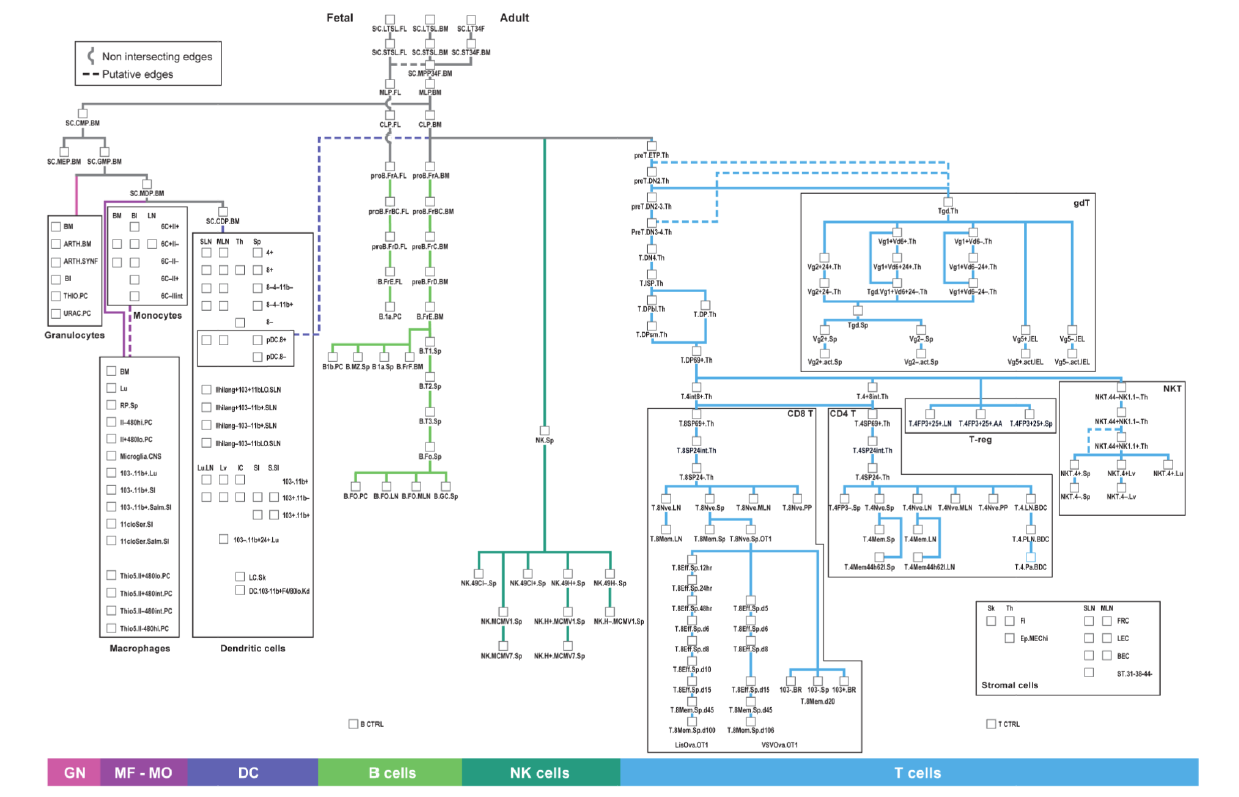
\includegraphics[width=0.9\textwidth]{Figures/Chapter3/immgen_lineage_tree.png}
\caption{\small{Lineage tree of the hematopoietic mouse cell types profiled by the Immunological Genome consortium ~\autocite{Joj2013}} }
    \label{fig:7}
\end{figure}

\subsubsection{Published ImmGen modules}

The ImmGen consortium has published modules of co-expressed genes which are organised into two levels of clustering, namely coarse and fine-grained ~\autocite{Joj2013}. In brief, 81 coarse-grained modules were initially defined using the hierarchical clustering method known as Super Paramagnetic Clustering (SPC) ~\autocite{Bla1996}. The SPC technique is based on the physical properties of an inhomogeneous ferromagnetic model and does not require input of a pre-defined value for the number of clusters between which the data must be split. Instead the algorithm assigns a Potts spin to each data point and attempts to identify the number that best fits the inherent structure of the dataset itself ~\autocite{Bla1996}. When run with default parameters SPC produced 80 stable clusters which were called coarse-grained modules C1-C80. Coarse module C81 contains the remaining unclustered genes and hence can be thought of as a "bin" module ~\autocite{Joj2013}. 

Subsequently, each coarse-grained module was partitioned to fine-grained modules. SPC could not further refine the coarse-grained modules and so affinity propagation clustering was employed ~\autocite{Fre2007}, using correlation as the affinity measure. Although not all genes could be included in this analysis, clustering resulted in 334 fine-grained modules, referred to in the text as fine modules F1-F334. On average each coarse-grained module contained 3.9 fine-grained modules ~\autocite{Joj2013}. 

The focus of this project is primarily centred around the transcriptional profiles of T cells alone and the ImmGen module database naturally seemed a good potential source of such T cell specific gene modules. Interestingly however, despite the plethora of data incorporated into the ImmGen analysis, only one course module, C18 (entitled "T-cell activation: TCR/CD3 complex genes, their downstream regulation"), appears to be specifically up-regulated in T cell subtypes (see Figure 3.2). This module contains 146 genes and was subdivided into 5 fine-grained modules (F90 - F94). 

\begin{figure}[H] 
    \centering
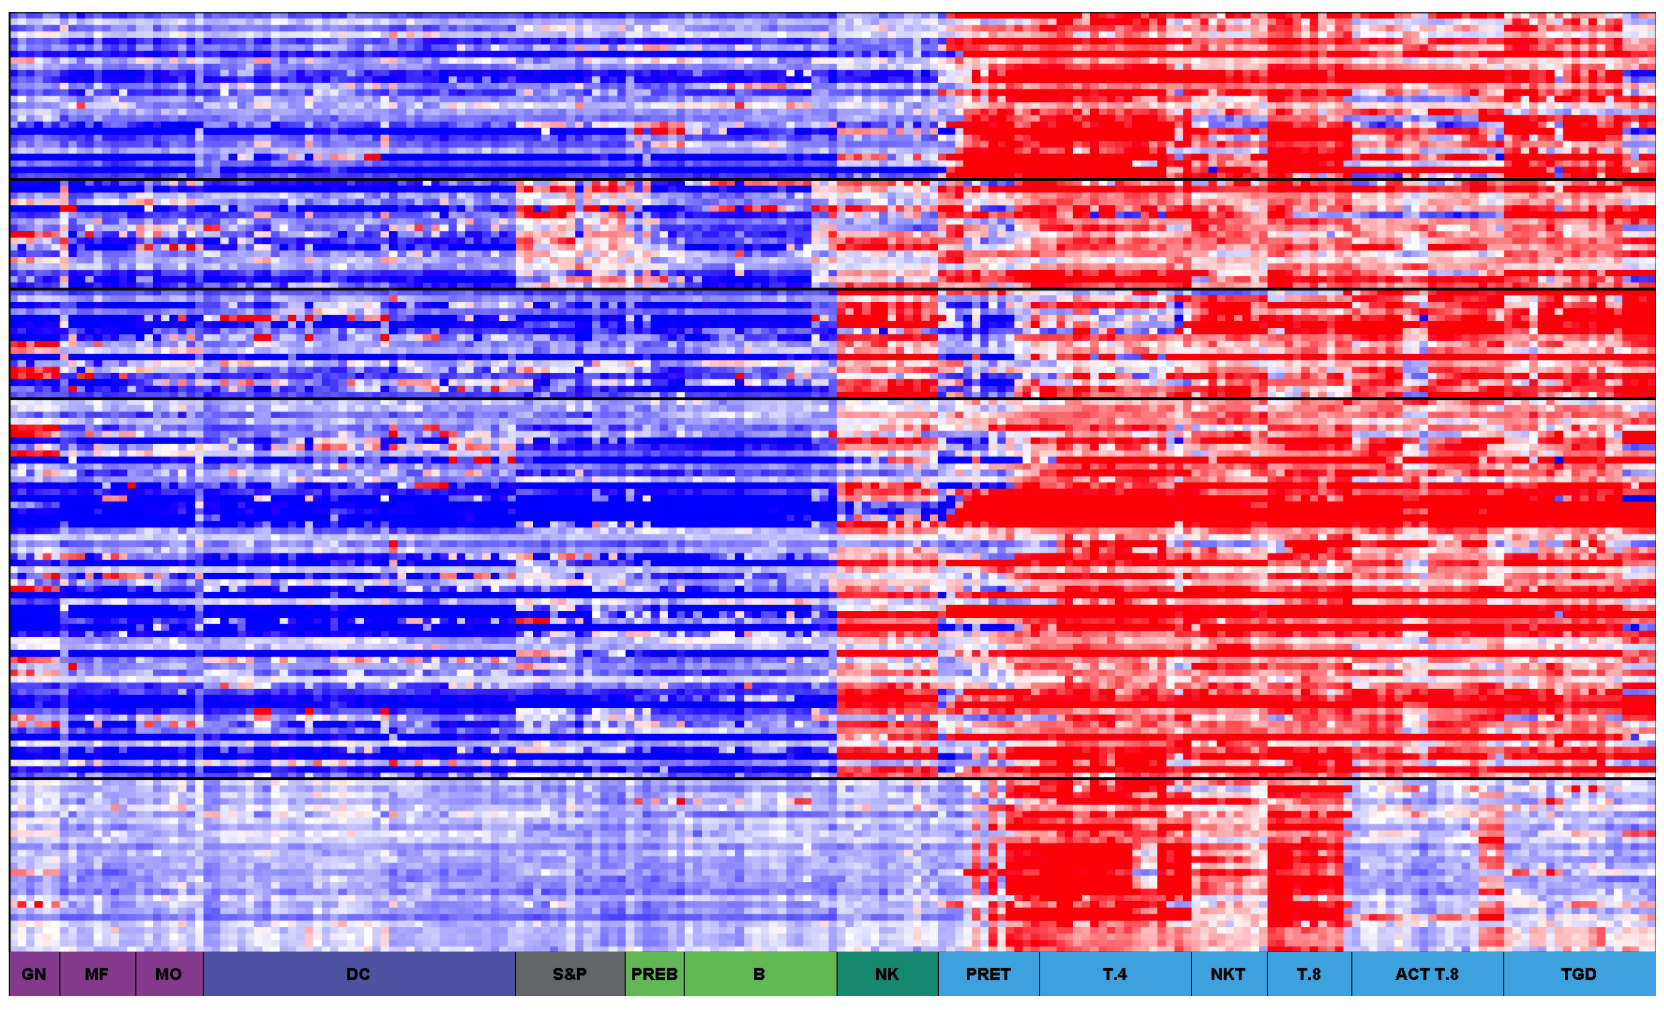
\includegraphics[width=0.7\textwidth]{Figures/Chapter3/C18_t_cell_activation.png}
\caption{\small{The mean centred expression of module C18 genes (rows) in each population of cells (column). Red denotes high expression levels, blue low expression levels. Major lineages are given at the bottom. Adapted from  ~\autocite{ImmGen}} }
    \label{fig:8}
\end{figure}

We therefore wondered whether by utilising the publicly available expression data from the ImmGen resource and extracting only those samples originating from T cell populations, we could re-cluster the genes in a manner that could generate a "Module Map" of T cell specific expression patterns. The following sections briefly summarise the data extracted for re-clustering as well as the various methods employed for the generation of gene modules. 

\subsubsection{T cell Dataset}

The microarray expression data used for gene clustering represents a subset of the complete ImmGen dataset ~\autocite{Joj2013}. Only T cell samples were included, resulting in an input data matrix consisting of 21755 gene expression values sampled across 89 samples. As outlined above, this T cell only dataset contained samples from $\alpha\beta$ cells, Tregs, $\gamma\delta$ cells and natural killer CTL populations. 

\subsection{Overview of clustering techniques employed}

\subsubsection{\underline{Weighted Gene Correlation Network Analysis (WGCNA)}}

In Chapter \ref{Chapter1} we briefly discussed the use of correlation matrices in the analysis of large datasets. Langfelder and Horvath built on this methodology to develop an R package to cluster highly correlated genes and analysing the functional properties of the resulting modules ~\autocite{Lan2008}. The WGCNA package they developed contains a comprehensive set of functions for performing a correlation network analysis of large, high-dimensional data sets. Functions available in the WGCNA package can be divided into several categories which also summarise the stages of a typical workflow when using this package to identify modules of genes within a microarray dataset. These categories are:

\begin{enumerate}
    \item Network Construction 
    \item Module Detection 
    \item Module and Gene Selection 
    \item Calculations of Topological Properties 
    \item Visualisation
    \item Interfacing with External Software 
\end{enumerate}

The following provides a brief overview of these analytical steps. 

\myparagraph{Network Construction}

In order to fully describe a gene network, it is necessary to calculate it's adjacency matrix which is a symmetric \textit{n} x \textit{n} matrix with entries in [0, 1] whose component \textit{$a_{ij}$} encodes the network connection strength between nodes \textit{i} and \textit{j}.. Computation of this matrix however requires that we first define the co-expression similarity \textit{$s_{ij}$} which is typically defined as the absolute value of the unsigned correlation coefficient between the profiles of nodes \textit{i} and \textit{j} as follows: 

\begin{equation}
    s_{ij}^{unsigned} = |cor(x_i, x_j)|
\end{equation}

One notable downside of taking the absolute value of the correlation is that biological information regarding whether genes are activated or repressed is usually lost. It is however possible to transform the similarity matrix defined in equation 3.1 in order to take account of the sign of the correlation between genes expression profiles: 

\begin{equation}
    s_{ij}^{signed} = 0.5 + 0.5cor(x_i, x_j)
\end{equation}

In the case of both $s_{ij}^{unsigned}$ and $s_{ij}^{signed}$, the similarity takes on a value between 0 and 1 but for two genes with opposing directions of expression profiles the unsigned similarity measure will equal 1, whereas it will be 0 if the signed measure is applied. \\

Given the similarity matrix as defined in equation 3.1 and 3.2, the corresponding adjacency matrix \textit{$a_{ij}$} is quantified by thresholding the chosen similarity matrix. 'Hard' thresholding (dichotomizing) the similarity measure $S = [s_{ij}]$ results in an unweighted gene co-expression network. Specifically an unweighted network adjacency is defined according to:

\begin{equation}
    a_{ij} = \bigg\{\frac{1 \text{ if } s_{ij} \geq \tau;}{0 \text{ otherwise}}
\end{equation}

where $\tau$ represents the "hard" thresholding parameter. Two genes are said to be linked i.e. \textit{$a_{ij}$} =1, when the absolute correlation between their expression profiles is greater than $\tau$. As the relationship between any two genes is classified in a binary manner, using a "hard" threshold can result in the loss of potentially biologically relevant information. However, WGCNA allows the user to instead apply a "soft" threshold which enables the continuous nature of the co-expression to be preserved by calculating a weighted network adjacency. This is achieved by raising the co-expression similarity to a power: 

\begin{equation}
    a_{ij} = s_{ij}^{\beta}
\end{equation}

$\beta \geq 1$ must apply for equation 3.4 to correctly calculate the adjacency. 

The calculation of adjacency matrices for both weighted and unweighted networks require the user to choose threshold parameters and one way this can be achieved within the WGCNA package environment is by applying the approximate scale-free topology criterion ~\autocite{Zha2005}.

\myparagraph{Module Detection}

One of the primary functions of the WGCNA package is to identify modules which are defined as clusters of densely interconnected genes. By default, the topological overlap measure (TOM) is used to calculate the network interconnectedness ~\autocite{Zha2005}. A key feature of WGCNA is that it does not require input of  \textit{a priori} defined gene sets, but instead identifies gene modules using unsupervised clustering. Hierarchical clustering using the standard R function hclust (described in a later section) is the default method. The blockwiseModules function facilitates network construction and module detection in large data sets by pre-clustering nodes into large clusters, or blocks, using a variant of k-means clustering. Hierarchical clustering is subsequently applied to each block in turn and gene modules are defined as branches of the resulting dendrogram. Lastly, modules wit highly correlated eigengenes are merged. 

Once modules have been detected, it is possible to summarise the expression profiles of genes within a given module using a variety of features. One option is to use the moduleEigengenes function which represents the expression profiles of genes within the \textit{q}-th module as \textit{$E^(q)$}, the first principal component of the expression matrix. The eigengene \textit{E} is equivalent to a weighted average expression profile.

\myparagraph{Module and Gene Selection}

The WGCNA package also contains functions to assist in identifying genes and modules that are likely to be biologically significant in a particular setting. In general terms, a gene significance measure is defined as a function \textit{GS} that assigns a non-negative number to each gene, \textit{i}. The higher \textit{GS\textsubscript{i}} the more biologically significant the gene. The interpretation of \textit{GS} measures will vary depending on the experimental context, but a high value could for example indicate pathway membership. Additionally, a microarray sample trait T can be used to define a trait-based gene significance measure as the absolute correlation between the trait and the expression profiles, i.e.:

\begin{equation}
    GS_{i} = |cor(x_i, T)|
\end{equation}


A measure of module significance can be calculated as the average gene significance, \textit{GS}, across the module genes (Figure 3A). Furthermore, when incorporating information relating to a sample trait \textit{T}, a measure of statistical significance between the module eigengene \textit{E} and the trait \textit{T} can be defined.

\myparagraph{Calculation of Topological Properties}

The WGCNA package implements several functions, including softConnectivity, intramodularConnectivity, TOMSimilarity, clusterCoef, and networkConcepts for computing gene network topological properties, many of which we defined in Chapter \ref{Chapter1}.

\myparagraph{Visualisation}

Both modular structure and network connections can be visualised in multiple ways within the WGCNA environment. To give an example, the co-expression module structure can be visualised by heatmap plots of gene-gene connectivity using the function TOMplot or as a multi-dimensional scaling plot. Relationships among modules can also be summarised by a hierarchical clustering dendrogram of their eigengenes, or a heatmap plot of the corresponding eigengene network. 

\myparagraph{Interfacing with External Software}

Once analysis of a dataset is complete, the WGCNA package contains a number of features to aid in integration of results with other network visualisation packages as well as gene ontology analysis software. For example, the R functions exportNetworkToVisANT and exportNetworkToCytoscape allow the export of networks in a format compatible with VisANT ~\autocite{Hu2008} and Cytoscape ~\autocite{Sha2003}, respectively. Gene lists compatible with Gene Ontology packages e.g. David ~\autocite{Den2003} are also easily generated. 

\subsubsection{\underline{Agglomerative Hierarchical clustering (Hclust)}}

Hierarchical clustering (also referred to as hierarchical cluster analysis) is a method of cluster analysis which seeks to build a hierarchy of clusters. The algorithm proceeds in a bottom-up manner whereby each object, in this instance gene, is initially considered as a single-element cluster (leaf). With each consecutive iteration, the two clusters that are the most similar are combined into a new bigger cluster (nodes). This procedure is repeated until all points are member of just one single big cluster (root). The result is a tree-based representation of the observations which is called a dendrogram. Hierarchical clustering in R was performed using the \textit{hclust()} function of the "cluster" package. 

\myparagraph{Determining Cluster Dissimilarity}

In order to decide which clusters should be combined a measure of dissimilarity between sets of observations is required. In most methods of hierarchical clustering, this is achieved by use of an appropriate measure of distance between pairs of observations (the metric), and a linkage criterion which specifies the dissimilarity of groups/clusters as a function of the pairwise distances of observations within them.

\underline{Metric}

The choice of an appropriate metric will influence the shape of the clusters, as some elements may be close to one another according to one distance and farther away according to another. For example, in a 2-dimensional space, the distance between the point (1,0) and the origin (0,0) is always 1 according to the usual norms, but the distance between the point (1,1) and the origin (0,0) can be 2 under Manhattan distance, $\sqrt{2}$ under Euclidean distance, or 1 under maximum distance.

\underline{Linkage Criteria}

The linkage criterion determines the distance between sets of observations as a function of the pairwise distances between observations. There are a number of different methods available to compute these distances, the most popular being: 

\begin{itemize}
    \item Maximum or complete linkage clustering: It computes all pairwise dissimilarities between the elements in cluster 1 and the elements in cluster 2, and considers the largest value (i.e., maximum value) of these dissimilarities as the distance between the two clusters. It tends to produce more compact clusters.
    \item Minimum or single linkage clustering: It computes all pairwise dissimilarities between the elements in cluster 1 and the elements in cluster 2, and considers the smallest of these dissimilarities as a linkage criterion. It tends to produce long, “loose” clusters.
    \item Mean or average linkage clustering: It computes all pairwise dissimilarities between the elements in cluster 1 and the elements in cluster 2, and considers the average of these dissimilarities as the distance between the two clusters. 
    \item Centroid linkage clustering: It computes the dissimilarity between the centroid for cluster 1 (a mean vector of length p variables) and the centroid for cluster 2.
    \item Ward’s minimum variance method: It minimizes the total within-cluster variance. At each step the pair of clusters with minimum between-cluster distance are merged.
\end{itemize}

\myparagraph{Hierarchical clustering and correlation based distance}

Typical statistical programming functions for hierarchical clustering use Euclidean distance measures as default metric. However, it is also possible to use correlation-based distance measures which are often more suited to the clustering of gene expression data. In such analyses, a pairwise correlation matrix between items is computed using the function \textit{cor()} which can calculate either “pearson”, “spearman” or “kendall” correlation method. Next, the correlation matrix is converted as a distance matrix and finally clustering can be computed on the resulting distance matrix.

Correlation-based distance considers two observations to be similar if their features are highly correlated, even though the observations themselves may lie far apart in terms of Euclidean distance.

It is important to note that, when the data are standardised, there exists a functional relationship between the Pearson correlation coefficient and the Euclidean distance:

\begin{equation}
d_{euc}(x,y) = \sqrt{2m[1-r(x,y)]}
\end{equation}
Where \textit{x} and \textit{y} are two standardised \textit{m}-vectors with zero mean and unit length.

\subsubsection{\underline{K-means}}

\myparagraph{Overview}

K-means clustering is an unsupervised learning algorithm, which iteratively assigns each data point to one of \textit{K} groups based on the features that are provided. Data points are clustered based on feature similarity. The results of the K-means clustering algorithm are as follows:

\begin{enumerate}
    \item The centroids of the K clusters, which can be used to label new data
    \item Labels for the training data (each data point is assigned to a single cluster)
\end{enumerate}

Each of the cluster centroids will possess a feature weight which can be used to qualitatively interpret what kind of group each cluster represents.  

\myparagraph{Algorithm}

The main idea of \textit{k}-means clustering, where Euclidean distance is used as a metric and variance is used as a measure of cluster scatter, is to define \textit{k} centroids, one for each cluster. The positioning of these centroids is a crucial variable as different locations will produce different results. The ideal is therefore for the centroids to be placed as far from one another as possible. Once initial positions have been fixed, the next step is to take each point belonging to the dataset and associate it to the nearest centroid. When all points have been assigned, the first step is completed and an early clustering has been completed. At this point it is necessary to re-calculate \textit{k} new centroids as barycenters of the clusters resulting from the previous step. After we have these \textit{k} new centroids, new assignments must be made between the same data set points and the nearest new centroid. A loop is thus generated within which the \textit{k} centroids change their location step by step until stable clusters have formed. 

\myparagraph{Choosing \textit{K}}

The algorithm described above finds the clusters and data set labels for a particular pre-chosen \textit{k}. To find the number of clusters in the data, the user must run the \textit{k}-means clustering algorithm for a range of values of \textit{k }and compare the results. In general, there is no perfect method for determining exact value of \textit{k}, but an accurate estimate can be obtained using a number of techniques.

One of the metrics that is commonly used to compare clustering results across different values of \textit{k} is the mean distance between data points and their cluster centroid. Since increasing the number of clusters will always reduce the distance to data points, increasing \textit{k} will always decrease this metric, to the extreme of reaching zero when \textit{k} is the same as the number of data points. Thus, the mean distance to the centroid as a function of \textit{k} is plotted and the "elbow point," where the rate of decrease sharply shifts, can be used to approximately determine the value of \textit{k} which best fits the data. It is important to note however that an inappropriate choice of \textit{k} may lead to poor results. 

\newpage

\section{Analysis of current/in-house GvHD (MataHari and B6) data}

\subsection{Differential gene expression (DE) analysis}

\subsubsection{Background}

Often when conducting microarray based experiments we are seeking to quantify which genes undergo changes in expression levels between sample groups. This methodology allows us to swiftly identify up- and down-regulated collections of genes in a given condition (either biological or experimental it nature). Each sample obtained from a microarray study will consist of a number of replicates and these will typically be summarised as the mean of the replicate expression levels. Thus in differential expression analysis, we are comparing mean differences in mRNA transcript production between the samples in question. 

\subsubsection{Statistical tests}

There are multiple approaches to statistically quantify whether expression level differences between samples are significant and each has it's own benefits and drawbacks. Almost all are focused on so called "two-class" problems and are only appropriate where the number of probes (\textit{p}) is much greater than the number of samples (\textit{n}). The method employed for establishing differentially expressed gene lists in this study is an empirical Bayes moderated t-statistic and it is this approach, together with the standard t-statistic upon which it is based, that will be covered here. 

\subsubsection{The t-statistic}

The basic formula for calculating a t-test for independent samples is:

\begin{equation}
t_g = \frac{\bar{X}_1 - \bar{X}_2} {\sqrt{\frac{\sigma^2_1}{N_1}\frac{\sigma^2_2}{N_2}}} \label{t-statistic}
\end{equation}

where $\bar{X}_i$ and $\sigma_i$ are the mean and variance of sample \textit{i} respectively. \\
\\
Whether the null hypothesis should be rejected is determined by comparing the value of $t_g$ obtained using the above calculation to the critical value. This critical value is defined as: 

\begin{equation}
t_{\alpha/2,n–p-1,}
\end{equation}

where $\alpha$ is the significance level, \textit{n} is the number of observations in the  sample, and \textit{p} is the number of variables.

If the absolute value of $t_g$ is greater than the critical value, the null hypothesis should be rejected in favour of the alternative. 

\myparagraph{Null hypothesis}

The null hypothesis of the t-test is that there is no statistically significant difference between the means of the two samples being compared i.e. 

\begin{equation}
H_o: \bar{X}_1 = \bar{X}_2 \label{t-statistic}
\end{equation}

\myparagraph{Assumptions}

The assumptions of the t-test are: 

\begin{enumerate}
    \item \textbf{Normally distributed data} - The populations from which the samples have been drawn should follow the normal distribution. 
    \item \textbf{Independence} - As is the case for all statistical tests of this nature, individual observations are assumed to be independent of one another.
    \item \textbf{Equal standard deviations} - The standard deviation of the populations should be equal.
\end{enumerate}

\myparagraph{Limitations}

The t-test has several limitations. Firstly, the variance in small samples can often be relatively "noisy" and this may have a substantial negative impact on the reliability of results. Secondly, while genes with small fold-change might be significant from a  statistical perspective, they may not be of interest biologically. 


\myparagraph{Computation in R} 

No computations of the t-test statistic were performed in this work with an adapted version, namely the empirical Bayes moderated t-statistic being preferred. 

\subsection{Fisher's Exact test}

\subsubsection{Background}

The Fisher's Exact Test of independence is a statistical tool used in cases where two nominal variables are measured and one wishes to assess whether the occurrence of of one of the variables is dependent upon the value of the other. The main application of this methodology is in situations where data exists in categorical format resulting from two-way classification of observations and so can be written in the form of a $2 \times 2$ contingency table. Thus this analysis represents a test of association between the two categories. Fisher's Exact Test is appropriate for analysis of small datasets and in this context is more accurate than the chi-squared or G-test methods. 

In this work we sought to quantify whether the observed number of differentially expressed genes assigned to a given module (X) was higher than that expected by chance. 

\subsubsection{Null hypothesis}

The null hypothesis of the Fisher's Exact Test is that the relative proportions of one variable are independent of the second variable, i.e. the proportions at one variable are the same for different values of the second variable. 

\subsubsection{Calculation of test statistic}

Consider the following generalised $2 \times 2$ contingency table:

\begin{center}
\begin{tabular}{ |c|c|c|c| } 
 \hline
  & \textbf{Not in module X} & \textbf{In module X} & Row Total \\ 
 \hline
 \textbf{Non DE} & a & b & \textit{a $+$ b} \\
 \hline
 \textbf{DE} & c & d & \textit{c $+$ d} \\
 \hline
Column Total & \textit{a $+$ c} & \textit{b $+$ d} & \textit{a $+$ b $+$ c $+$ d ($=$n)}\\
\hline
\end{tabular}
\end{center}

Given this notation, Fisher showed that the probability of obtaining any such set of values could be established using the hypergeometric distribution as follows:

\begin{equation}
p = \frac{\binom{a+b}{a} \binom{c+d}{c}} {\binom{n}{a+c}} = \frac{(a+b)!(c+d)!(a+c)!(b+d)!}{a!\, b!\, c!\, d!\, n!} \label{hypergeo}
\end{equation}

When substituted with actual data, equation \eqref{hypergeo} gives the exact hypergeometric probability of obtaining the observed arrangement of the data, assuming the marginal totals (i.e., assuming the row and column totals shown in the margins of the table are given), under the null hypothesis that genes are all equally likely to be differentially expressed whether they form part of module X or not.  

Although application of the above formula facilities calculation of the exact probability of any arrangement of the \textit{n} observations into the four table cells, Fisher proved that in order to generate a significance level for the test result it is only necessary to do so for cases where two linked conditions are met. These are:

\begin{enumerate}
    \item  The marginal totals are the same as in the observed table;
    \item and among those, only where the arrangement is as, or more extreme than the observed arrangement
\end{enumerate}

Having computed these additional probabilities, the significance of the observed data can be obtained by summation of these values together with that calculated using the actual frequencies. This is a one-tailed test however which, in practice, is rarely suitable. It is virtually always necessary to conduct a two-tailed test, which in addition to the calculations outlined above, requires the inclusion of tables with combinations as equally extreme as the observed but in the opposite direction. This is something of a challenge as there is no clear cut threshold for what values should qualify as "extreme". There are multiple approaches to address this issue, the most common of which is to sum the probabilities of all combinations possessing probabilities lower than, or equal to, that of the observed data. 

\subsubsection{Assumptions}

Fisher's Exact Test carries two main assumptions, namely: 

\begin{enumerate}
    \item \textbf{Independence} - Samples are assumed to be independent of one another. The same should be true of the variables used for classification. 
    \item \textbf{Fixed totals} - Although often not adhered to in biological studies, this test is only actually exact when both the row and column totals are fixed or "conditioned". 
\end{enumerate}

\subsubsection{Limitations}

Whilst the Fisher's Exact Test may seem well suited for assisting in our search for potential enrichment of differentially expressed genes within module lists, we believe there is one potentially key feature that it is lacking. This statistical test does not take any account of the relative direction or size of the change in expression for differentially expressed genes within a given module. We believed that incorporating this aspect of the dataset could potentially add significant power to our analyses, as well as offering the opportunity to uncover more biologically relevant associations. 

\subsubsection{Computation in R} 

All computations of the Fisher's Exact Test statistic were performed in R using the fisher.test() function of the \textit{stats} package. 

\subsection{Module-based differential expression analysis - New refined testing protocol}

\subsubsection{Background}

In order to quantify potentially significant associations of gene modules (specifically those derived from WGCNA or similar algorithms) between tissue types and/or between conditions, we developed a gene based association test that, unlike aforementioned statistical tests of association, incorporates information regarding the magnitude and sign of the differential expression effect size observed for each gene.

\subsubsection{Calculation of test statistic}

Given that the purpose of this test is to assess whether genes are consistently over-expressed in a set of cases compared to controls, the initial step is to transform a gene's \textit{p}-value into a chi-squared statistic $X_\textit{i}$ with one degree of freedom, at which point the \textit{T} statistic can be calculated by summing, for all genes, the $X_\textit{i}$, if $X_\textit{i}$ is positive, or 0, if it is negative. Under the null, the distribution of this $X_i$ is determined by applying the assumption that for any given gene, the chance of under- or over-expression is 50\%. An important feature of this testing protocol is that, if it is known that this assumption does not hold for a particular dataset, this parameter can be refined by computing the genome-wide probability of over-expressed genes. Whatever the genome-wide proportion of over-expressed genes, the corresponding probability of observing \textit{K} over-expressed genes among the \textit{n} genes that form a module can be computed using a binomial distribution. As any given \textit{K} represents the sum of \textit{K} one degree of freedom chi-square distributions, the statistic \textit{T} is chi-squared with \textit{K} degrees of freedom. The probability of observing a test statistic greater than the observed value \textit{T} can then be computed using a weighted sum of probabilities, summing over all possible values of \textit{K}. 

Whilst the above explanation is based upon the proportion of over-expressed genes, the calculations are equivalent if all genes are predicted to be under-expressed. If a mixture of over- and under-expressed genes is expected, the \textit{T} statistic is then summed over all genes in an appropriate manner to reflect the said combination.

\subsubsection{Data simulations}

Having developed the module-based refined testing protocol for differential expression datasets, we analysed its behaviour and performance on simulated gene module data. To this end we generated two simulated datasets, one to assess how our module-based test handles data matching the null, where the gene-based "direction of effect" within a module is not relevant and a second, alternative, dataset where a proportion of genes within a module exhibit a skewed direction in terms of the sign ($+/-$) of the log(fold change) in expression levels between artificially simulated "conditions". The next two sections provide details of the simulated datasets (16000 "genes") used to test the performance of our module-based test as well as a summary of the observed findings. 

\myparagraph{Simulating under the null}

We expect that when supplied with data consisting of uniformly distributed \textit{p}-values and direction (i.e. genes have a 50-50 chance of going up/down), our \textit{T} statistic should behave as a chi-squared with two degrees of freedom. To determine whether this predicted distribution of \textit{p}-values was observed, we generated a dataset of 16000 data points, each with a \textit{p}-value and assigned direction drawn from uniformly distributed populations (min = 0, max = 1 for \textit{p}-values, min = -1, max = 1 to acquire direction sign). "Modules", each containing 200 simulated gene data points were sampled, put through the refined testing analysis and the resulting distribution of test statistic \textit{p}-values plotted against the corresponding expected order statistics (using the \textit{qq.chisq} function of the \textit{snpMatrix} R package). This plot is shown in Figure 3.3 below. 

\begin{figure}[H] 
    \centering
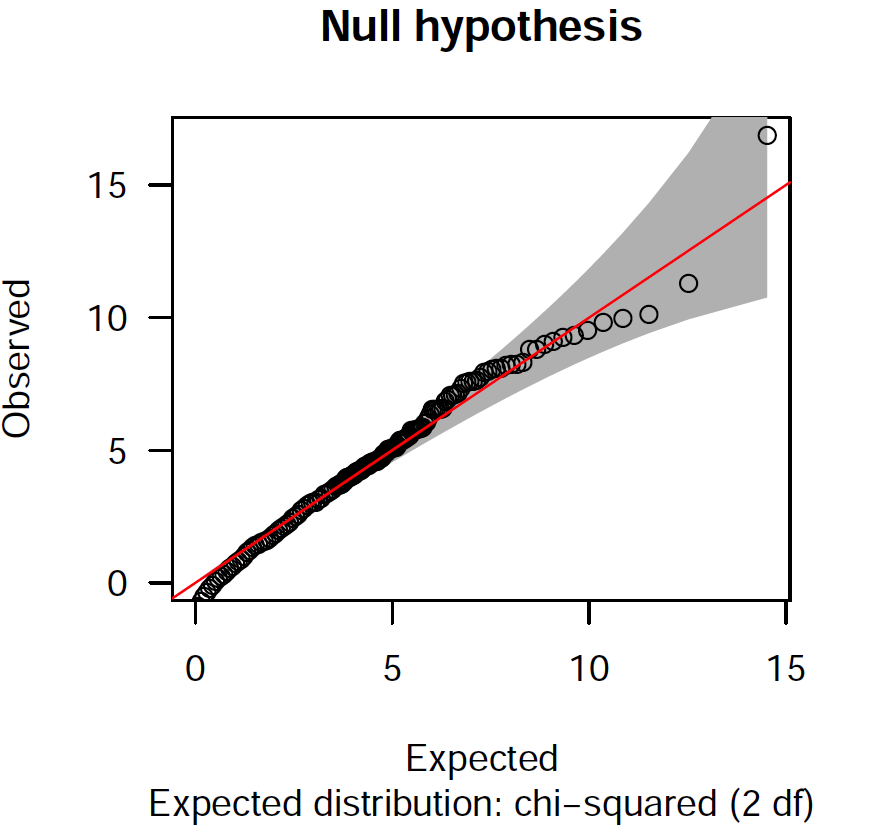
\includegraphics[width=0.5\textwidth]{Figures/Chapter3/simulated_null_skewedDir.png}
\caption{\small{Distribution of module-based refined test statistic \textit{p}-values simulated under the null plotted against the corresponding expected order chi-squared statistics (two degrees of freedom)} }
    \label{fig:9}
\end{figure}

It is evident from the above plot that, when provided with uniformly distributed data (the null situation), the \textit{T} statistics generated by our test are indeed a good fit to a chi-squared with two degrees of freedom. This is an encouraging and reassuring result as it indicates that our analysis is not falsely amplifying, or worse still manufacturing, significant \textit{p}-values when none are present in the test dataset. 

\myparagraph{Simulating under the alternative}

To establish how our module-based test performed on data fitting the alternative hypothesis where the direction of effect is skewed for the portion of genes that are significantly up-regulated/over-expressed, we created a simulated dataset similar to that used to evaluate our statistic under the null, but this time while the \textit{p}-values remained uniformly distributed the proportion of up-regulated genes varied (see Figure 9). Again, 16000 data points were generated, each with a \textit{p}-value selected at random from a uniformly distributed population as outlined above, but 40\% of the dataset had its positive directional skew enhanced to a varying degree resulting in between 50\% and 95\% of those genes to mimic over-expression. As for the "null" simulations, gene "modules", each containing 200 simulated genes were sampled, tested according to our module-based protocol and Figure 3.4 shows the resulting \textit{p}-values plotted against the relative expected chi-squared statistics (using the same \textit{qq.chisq} function as previously).

\begin{figure}[H] 
    \centering
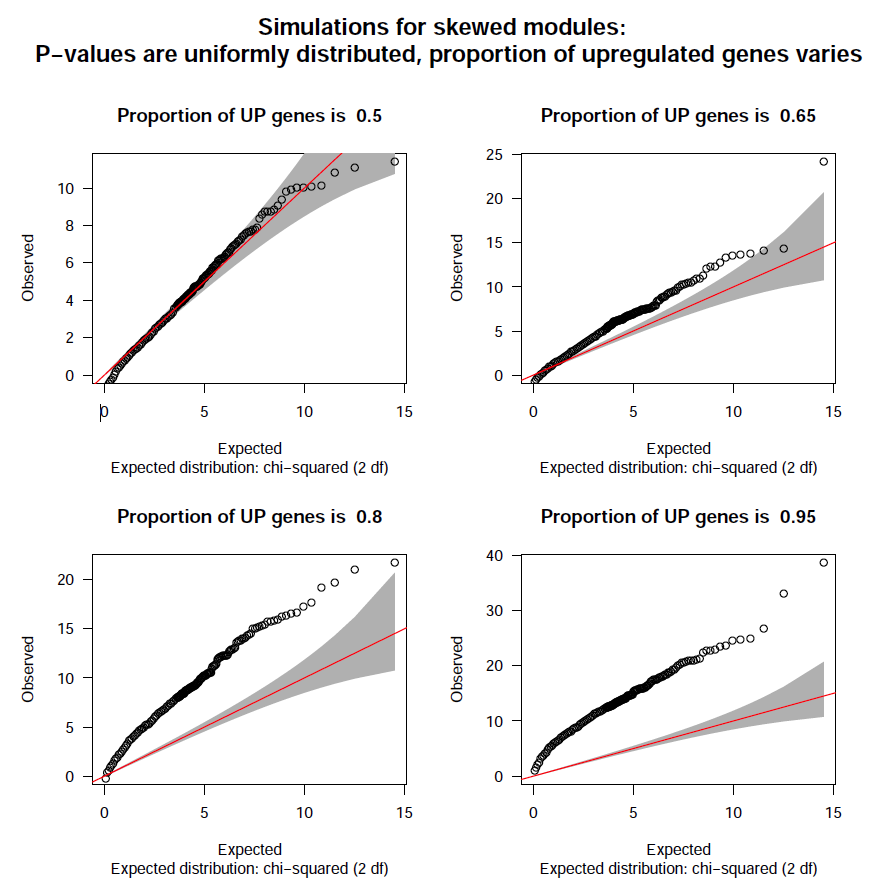
\includegraphics[width=0.8\textwidth]{Figures/Chapter3/simulated_alternative_skewedDir.png}
\caption{\small{Distribution of module-based refined test statistic \textit{p}-values simulated under the alternative plotted against the corresponding expected order chi-squared statistics (two degrees of freedom)} }
    \label{fig:10}
\end{figure}

As can be seen from inspection of Figure 3.4, when the proportion of up-regulated genes is 0.5 our test generates \textit{p}-values highly similar to those seen in the null simulations (Figure 3.3). Naturally the distribution of points is not identical due to random sampling. However, as the module-based proportion of up-regulated genes increases, it can be seen that our \textit{T} results gradually deviate from those expected under a chi-squared with two degrees of freedom. Thus our refined association test successfully enhances the significance of modules containing a high proportion of genes with a common change in expression levels (either up- or down-regulated). The fact that the degree to which the significance is enhanced depends upon the inherent skew in relative proportions of over- and under-expressed genes in a few module dramatically increases the power of this statistical methodology. 



\chapter{Mapping the T-cell transcriptional landscape: can we utilise  currently available clustering techniques  to define a module map?} % Main chapter title

\label{Chapter4} % For referencing the chapter elsewhere, use \ref{Chapter1} 

%----------------------------------------------------------------------------------------
\section{Overview}

This Chapter details the results of reclustering of the ImmGen T cell dataset (for an overview of the data please see Chapter \ref{Chapter1}. Three clustering algorithms were implemented, specifically WGCNA, Hclust and K-means. All three methodologies are described in Chapter \ref{Chapter3}. The primary aim of this work is to compare and contrast how different algorithms behave when tasked with clustering the same data and to attempt some quantification of the biological relevance of the module sets produced in each case. The following sections summarise some of the key steps/decisions taken during clustering as well as comparing how the output modules from each algorithm relate to the original Coarse modules published by the ImmGen consortium. 

\section{Weighted Gene Correlation Network Analysis (WGCNA)}

The first technique utilised to perform reclustering of the T cell data set was WGCNA. An outline of the steps undertaken within this work flow is provided in Chapter \ref{Chapter3} and the following plots provide a summary of the key stages in module generation. One of the initial stages in the process of module generation using WGCNA is examination of the samples following hierarchical clustering. The purpose of this analysis is to provide a visual means by which any potential outliers can be identified and subsequently removed to avoid skewing of later gene clustering results. As is evidenced by Figures 4.1 and 4.2, the T cell dataset appeared to contain a single outlier sample (X.T\_DPbl\_Th.) which was removed by cutting the dendrogram at a height of 51,000. Removal of this sample did not result in the loss of any other data and resulted in the sample clustering dendrogram appearing more suitable for further analysis i.e. all samples were clustered with at least one other on a given branch (Figure 4.2). 

One particularly useful feature of the WGCNA package is that it is very easy to input trait information which can subsequently be linked with the modules produced in order to analyse which if any of the gene clusters are enriched in particular samples/experimental groups. Similar mapping to trait data is also facilitated when examining the distribution of clustered samples as is shown in Figure 4.3. As is evident from this figure, in the majority of cases samples are clustered with neighbours that are of the same original cell type. Over half of the dataset is comprised of $\alpha\beta$ T cell samples and whilst they have not remained in a single cluster, most are contained within one of three groups suggesting that there is a degree of similarity in the expression profiles of these individual cells. Indeed, all three T cell subtype samples were split into multiple clusters and in several cases $\alpha\beta$ samples were clustered together with $\gamma\delta$ relatives suggesting that these two populations share highly similar characteristics in terms of gene expression patterns. Given the processes of differentiation described in Chapter \ref{Chapter2} this is an unsurprising observation, although the apparent separation of some samples within each subtype is a little unexpected. It is true that most but not all of the samples within the ImmGen database represent activated cells and so it may be that this has some bearing both on the dissimilarities within cell subtypes as well as the similarity of some $\alpha\beta$ and $\gamma\delta$ samples. 

\begin{figure}[H] 
    \centering
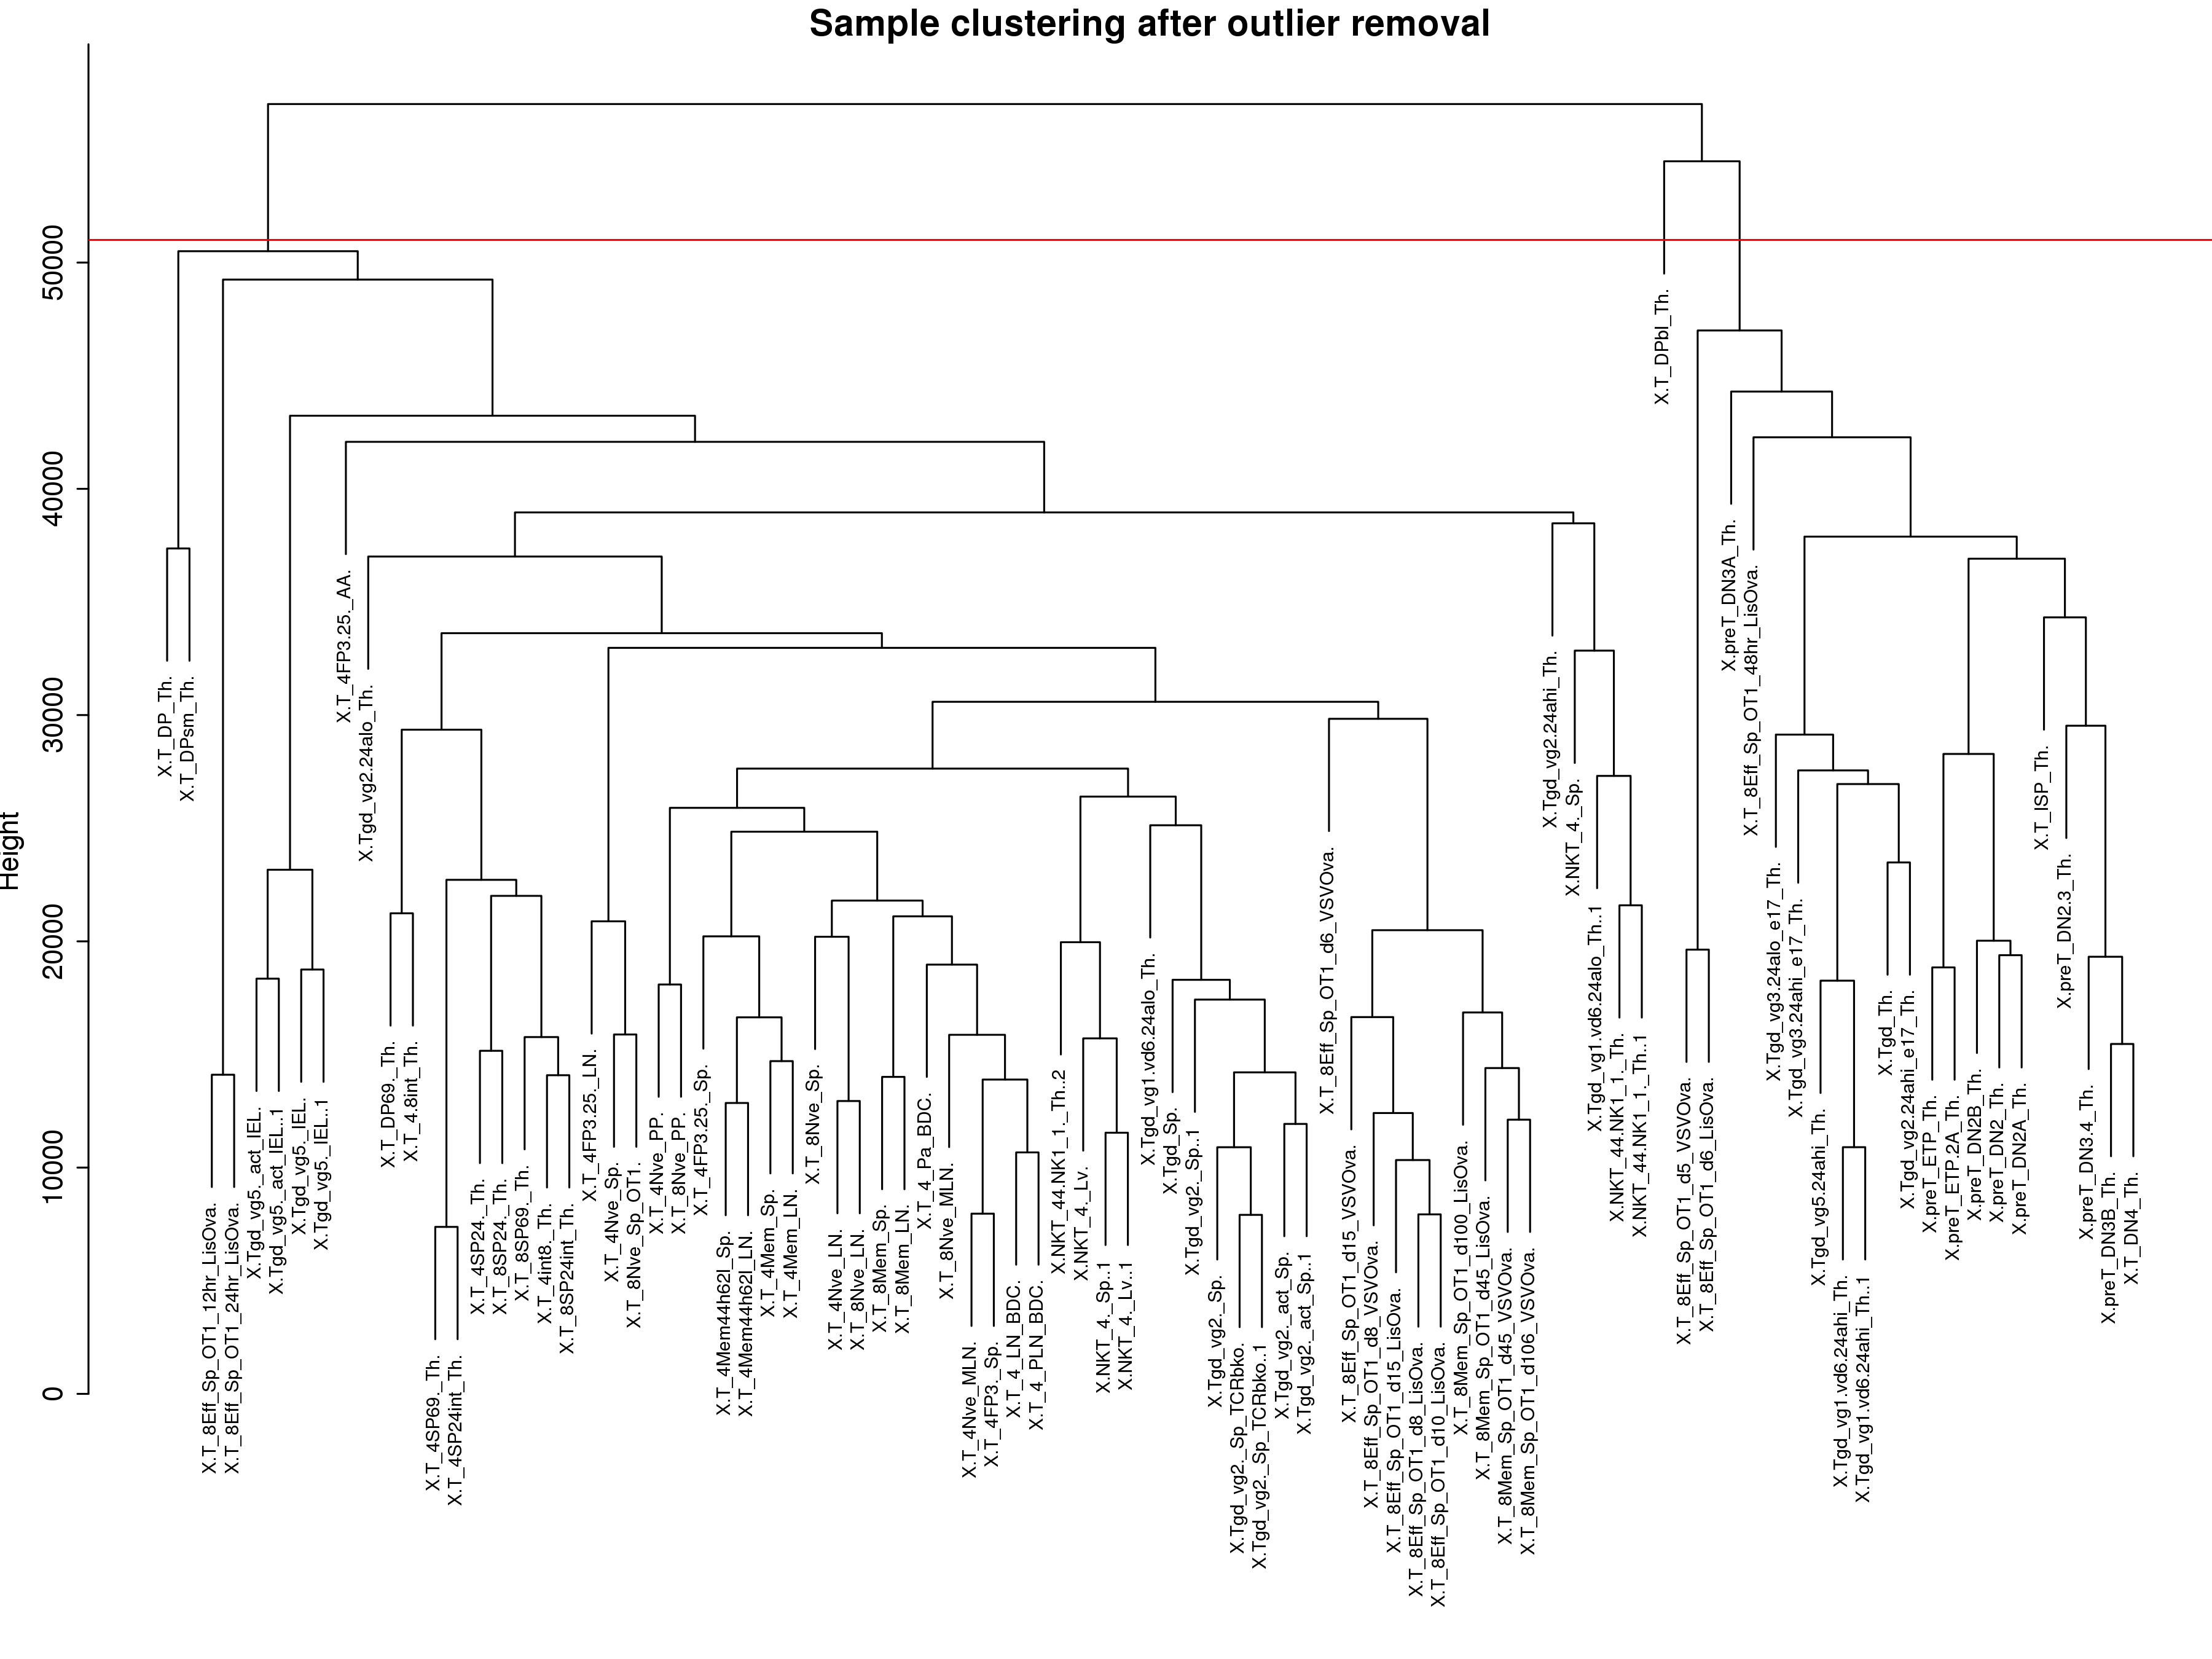
\includegraphics[width=1\textwidth]{Figures/Chapter4/WGCNA/tcell_immgen_data_sampleClustering.png}
\caption{\small{Dendrogram of ImmGen T cell dataset showing the distribution of samples following hierarchical clustering and the resulting presence of an outlier sample. The red line indicates the cut height used for the removal of this outlier. } }
    \label{fig:11}
\end{figure}

\begin{figure}[H] 
    \centering
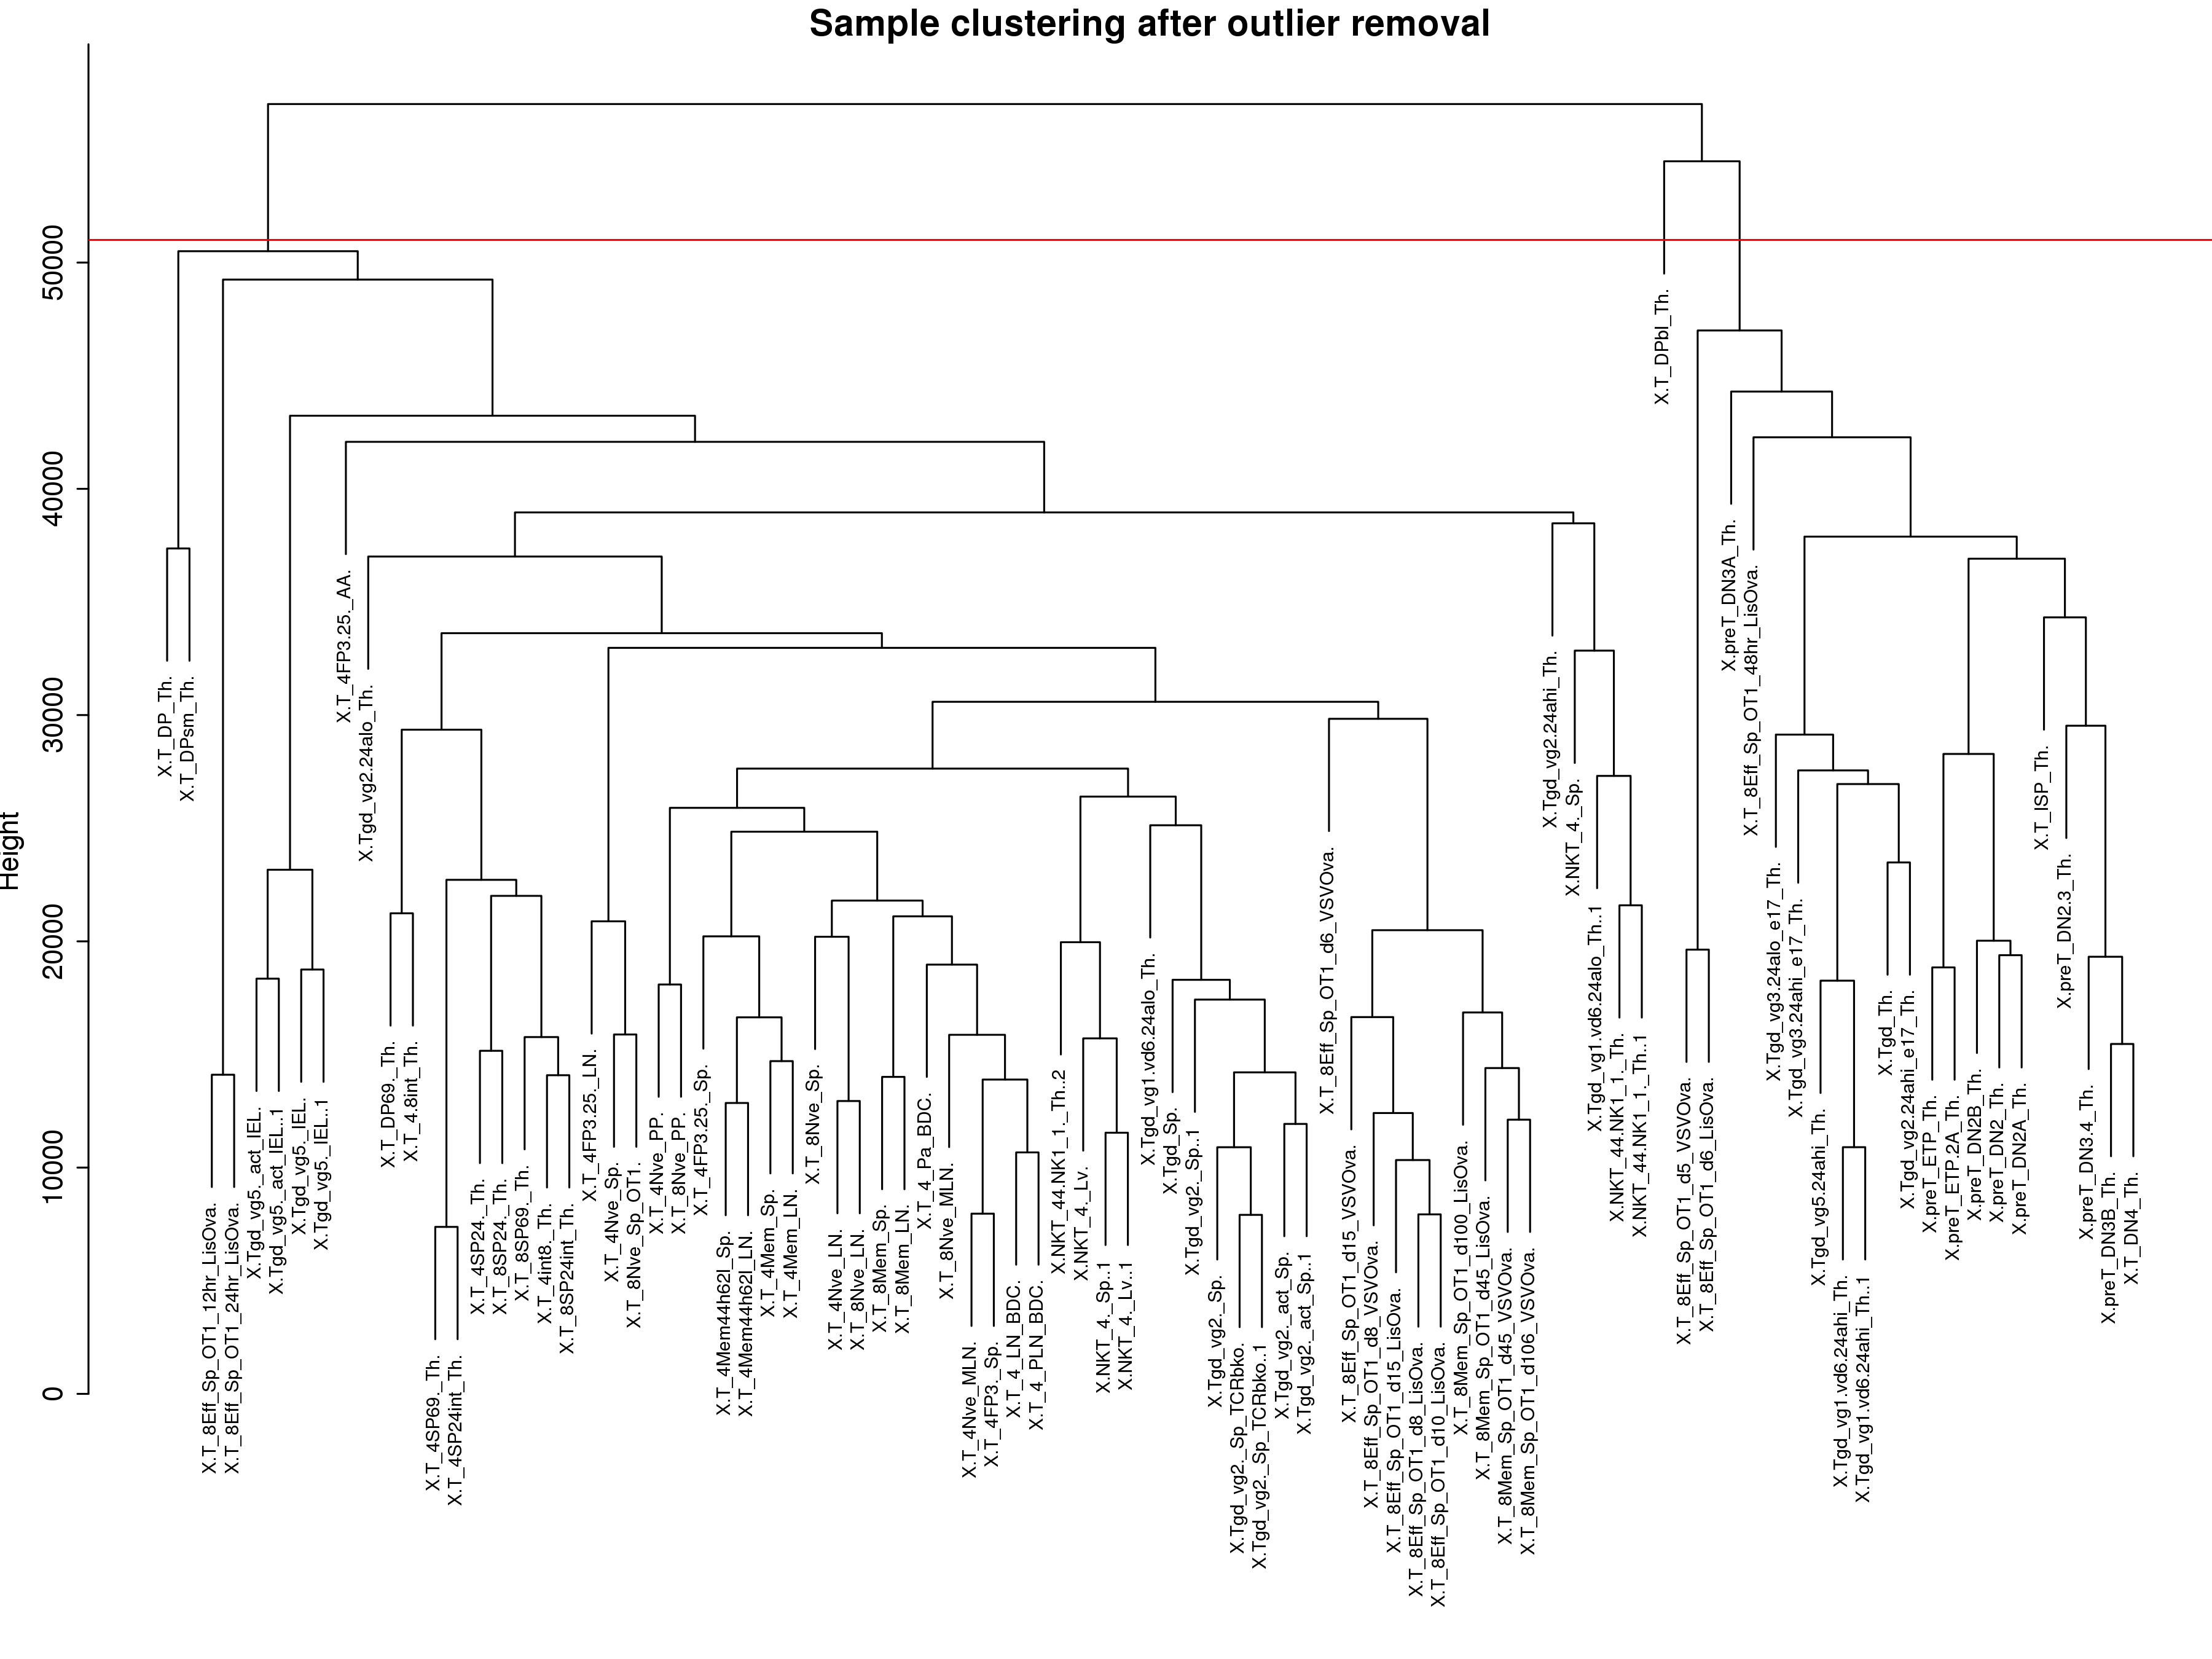
\includegraphics[width=1\textwidth]{Figures/Chapter4/WGCNA/tcell_immgen_data_sampleClustering.png}
\caption{\small{Dendrogram of ImmGen T cell dataset samples following outlier removal} }
    \label{fig:12}
\end{figure}

\begin{figure}[H] 
    \centering
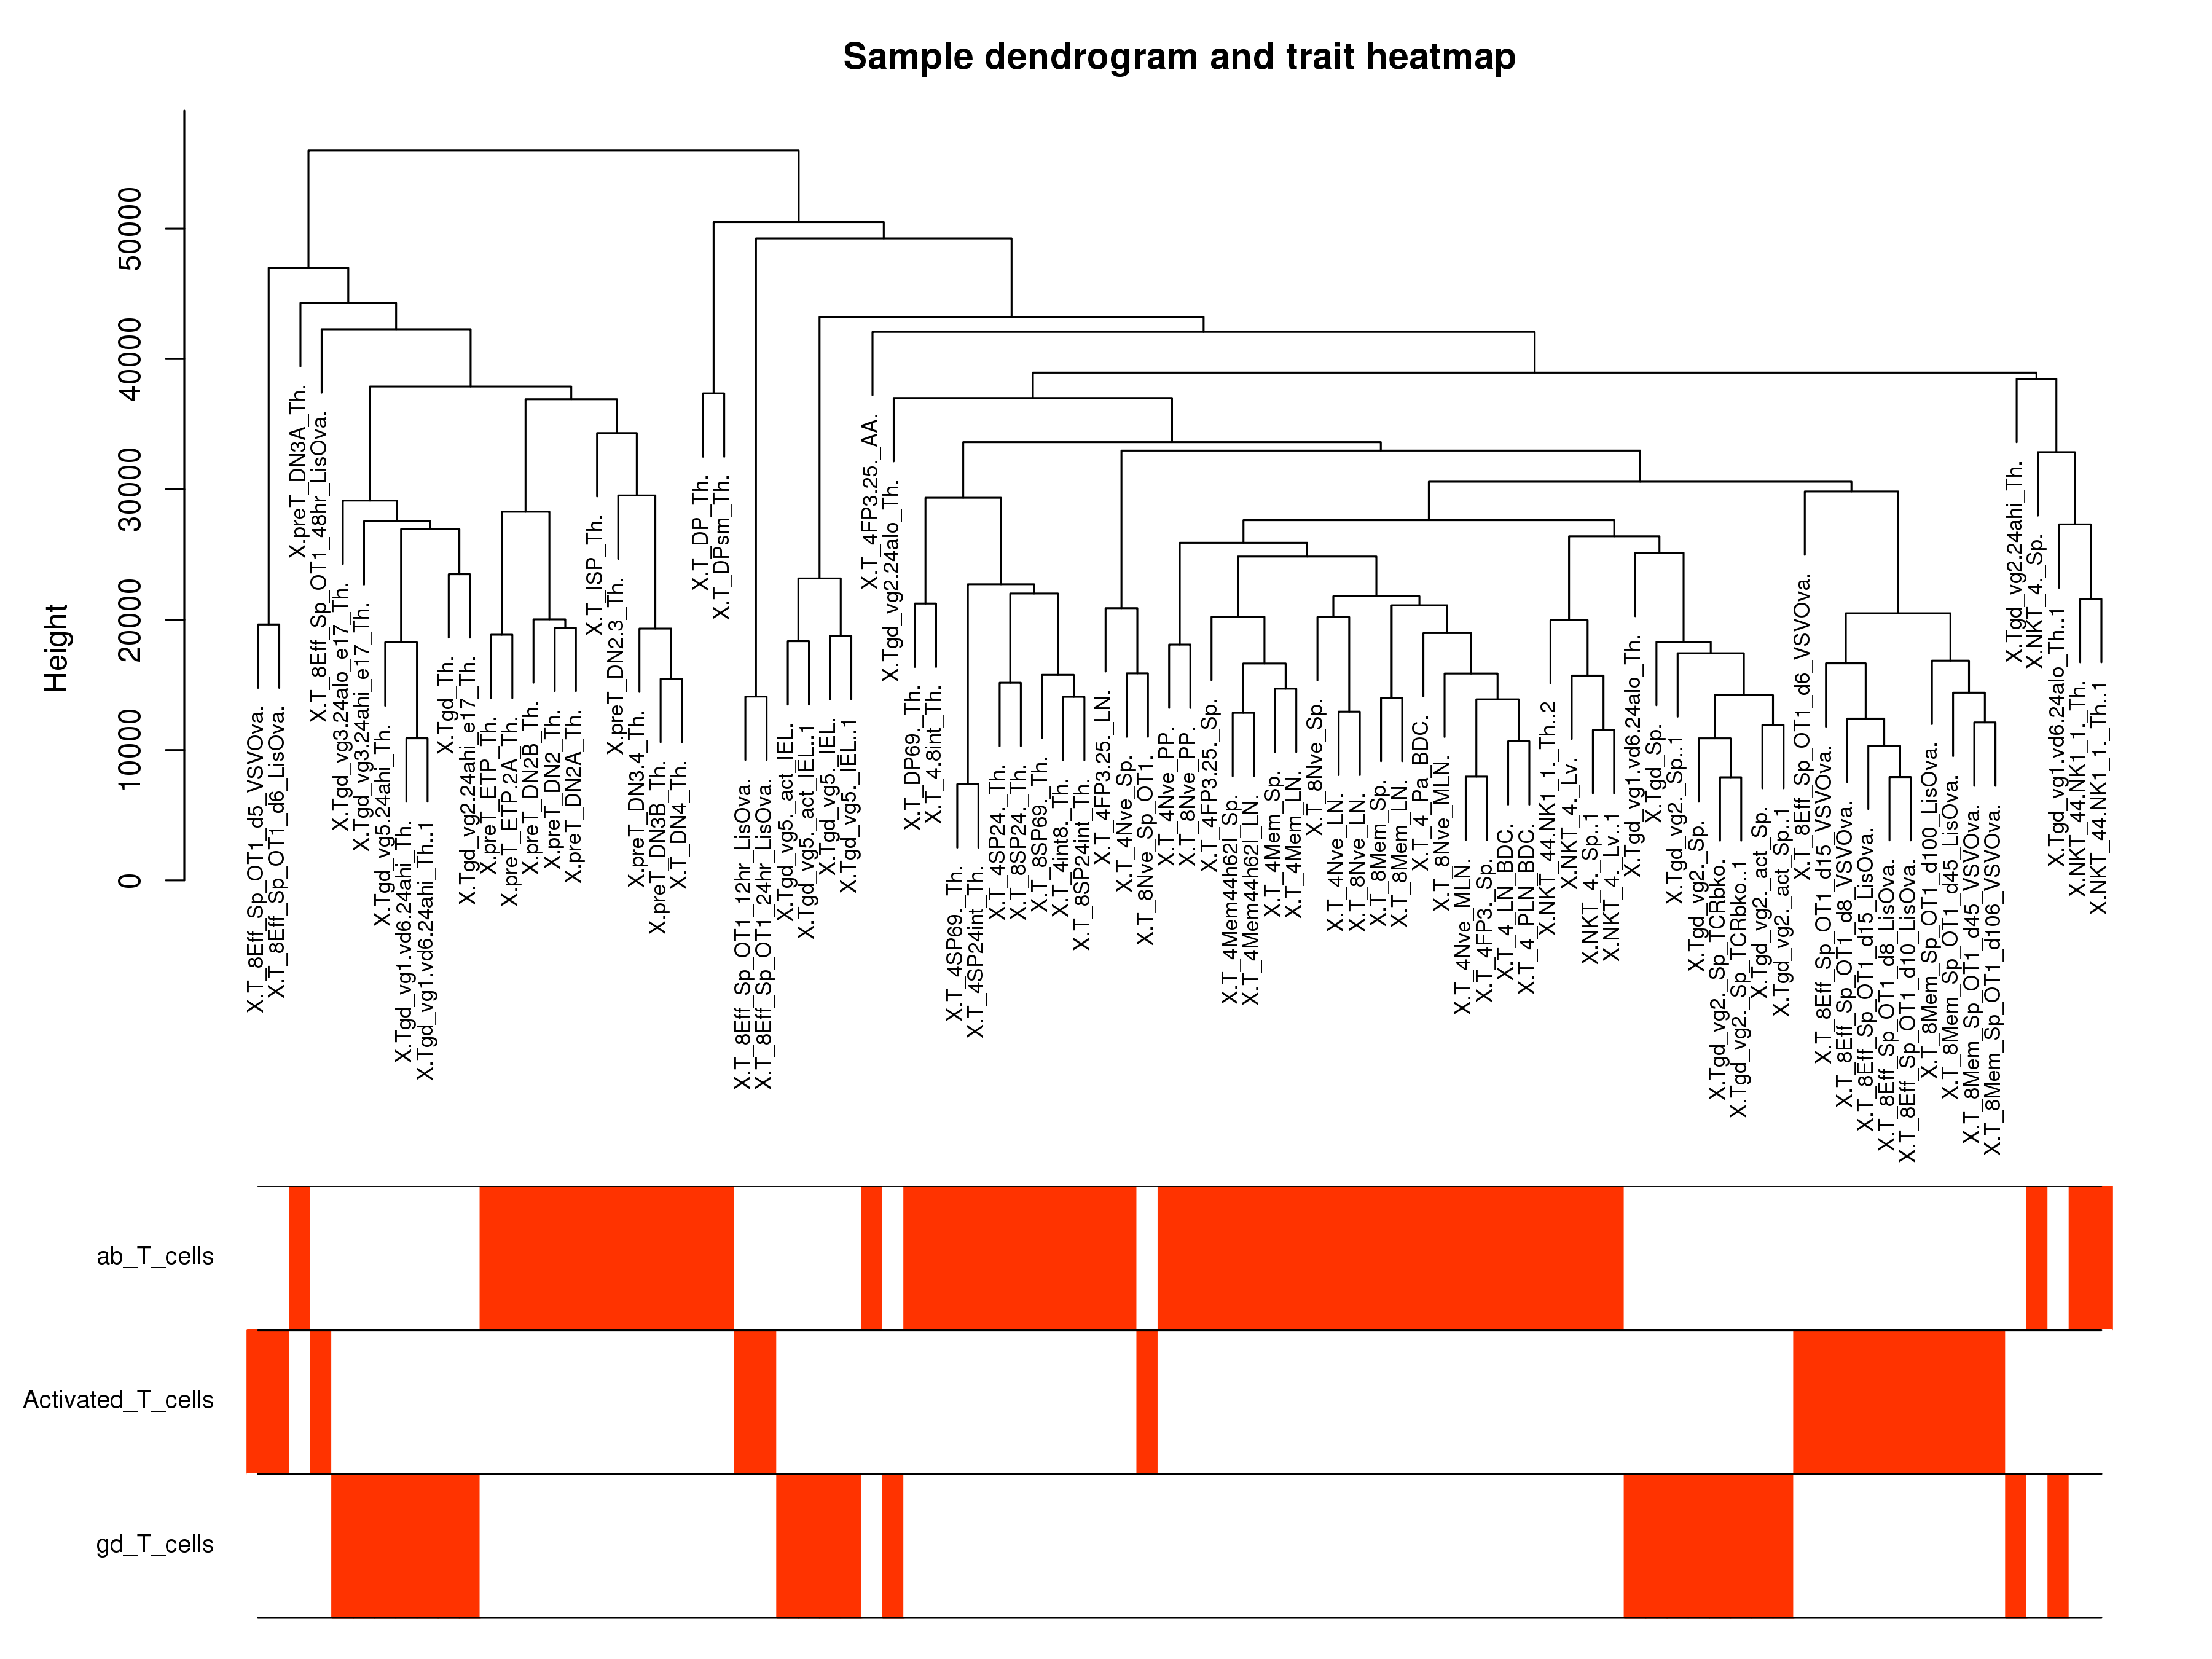
\includegraphics[width=1\textwidth]{Figures/Chapter4/WGCNA/tcell_immgen_data_dendrogram_plus_traits.png}
\caption{\small{ImmGen T cell dataset sample dendrogram with associated trait information displayed beneath.} }
    \label{fig:13}
\end{figure}

Following visual examination of the data and the necessary pre-processing steps including selection of the thresholding power (see Chapter \ref{Chapter3}) which for this dataset was selected as 39 based on modelling the scale free topology, all genes were clustered using the cutreeDynamic function of the WGCNA package. 204 gene modules were produced as a result of this gene clustering with size ranging from 1 to 6344 genes per module. Naturally, a gene module consisting of 1 or even several genes is not going to be biologically relevant and so all modules containing less than 5 genes were removed from further analysis. Similarly, it is difficult to see how a module comprising thousands of genes is likely to represent a cohesive collection of interacting genes and so the two modules whose sizes were greater than 1000 genes were also ignored in subsequent work. As mentioned in Chapter \ref{Chapter3}, WGCNA offers the option to summarise each module identified by its eigengene and Figure 4.4 shows the dendrogram of all module eigengenes produced by the gene clustering algorithm. It is clear from this plot that a number of the eigengenes are extremely closely "related" and as per the recommended analytical procedure, modules whose eigengenes were below 0.05 on the dendrogram were merged using the in built function mergeCloseModules.

\begin{figure}[H] 
    \centering
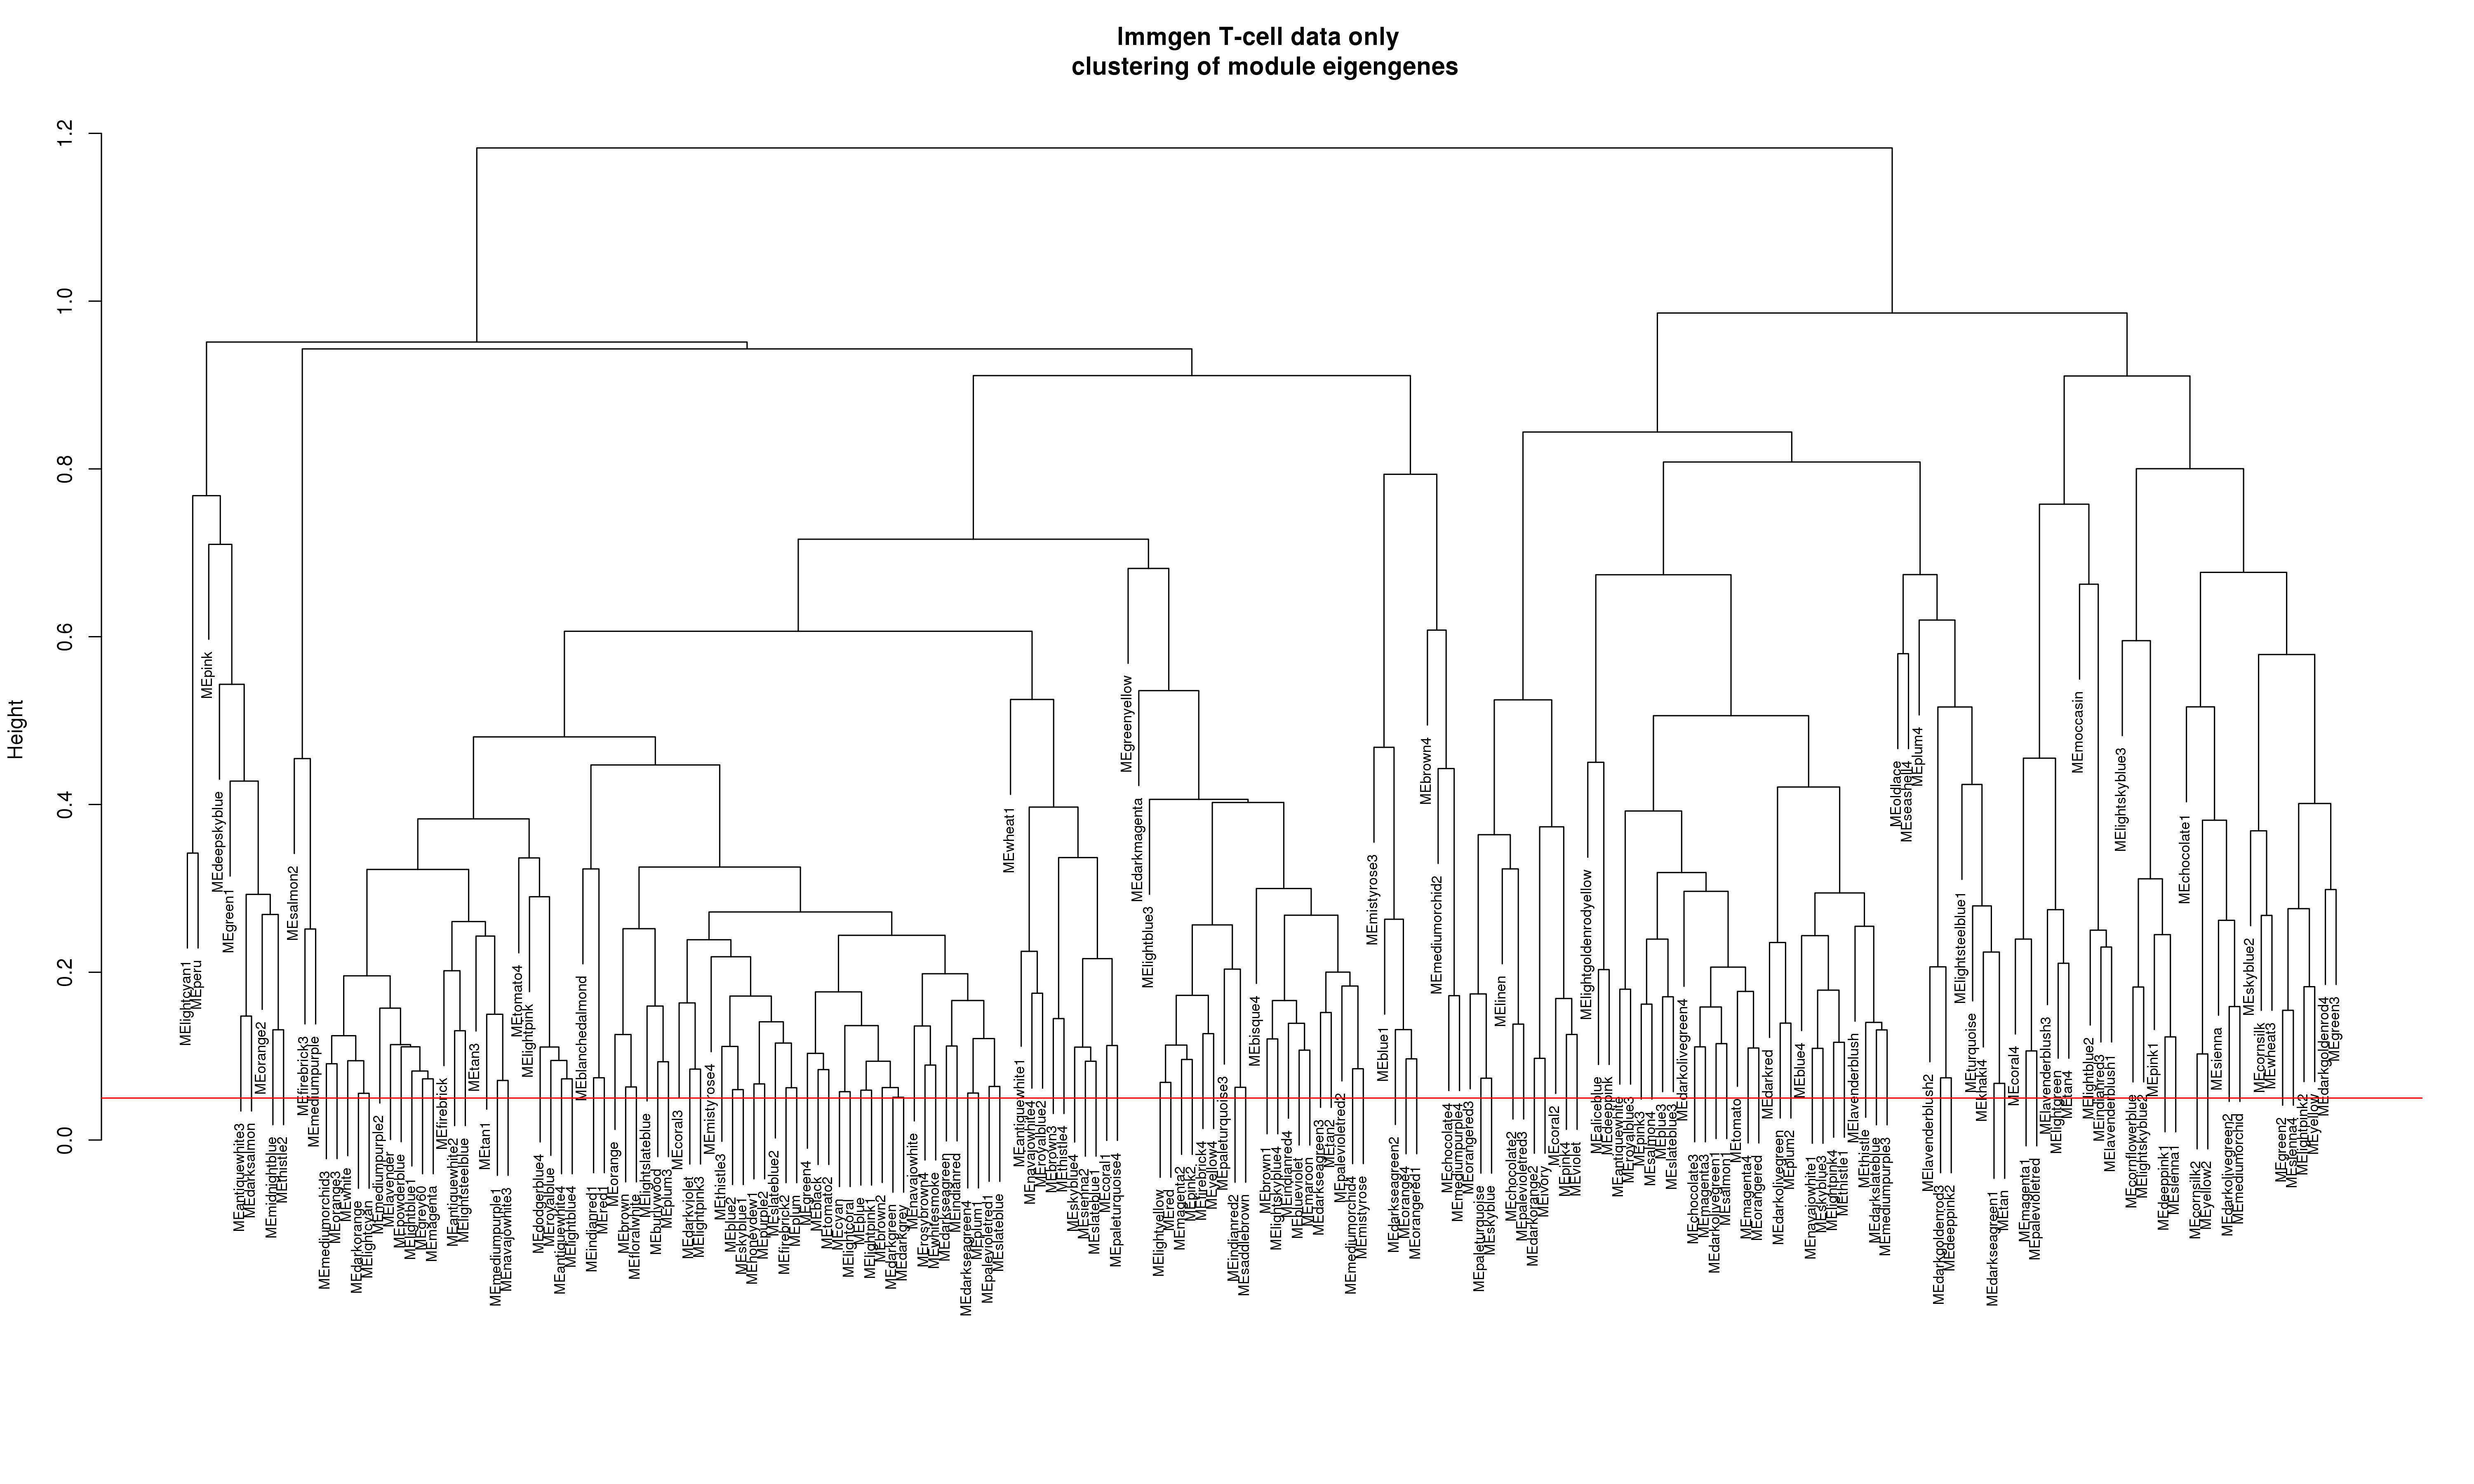
\includegraphics[width=1\textwidth]{Figures/Chapter4/WGCNA/tcell_immgen_data_module_eigengene_clustering.png}
\caption{\small{Dendrogram of the module eigengenes produced by clustering using WGCNA. The red line depicts the threshold below which modules were merged to avoid the generation of modules too small to be of biological relevance. } }
    \label{fig:14}
\end{figure}

One particularly useful feature of the WGCNA package is the ability to plot correlations between gene modules and sample traits in the form of a heatmap. This enables straightforward evaluation of whether any given module is associated with a particular trait and this is extremely useful when attempting the early stages of clustering quality evaluation and module annotation. Given the large number of modules produced in this particular analysis, it is not feasible to discuss each module individually. However, the module - trait heatmap shown in Figure 4.5 does provide a general overview of how the distribution of gene modules relates back to the T cell subtypes included in this dataset. Interestingly, the majority of correlations are very weak which would indicate that the genes they are comprised of may not all originate from a single cell type. There are a few exceptions, notably a collection of modules strongly correlated with the Activated T cell samples, but in general the results are disappointing. Without performing an in depth analysis examining each of the 204 gene modules it is difficult to determine whether poor clustering results or the splitting of tightly clustered genes across multiple modules may be the cause. 

\begin{figure}[H] 
    \centering
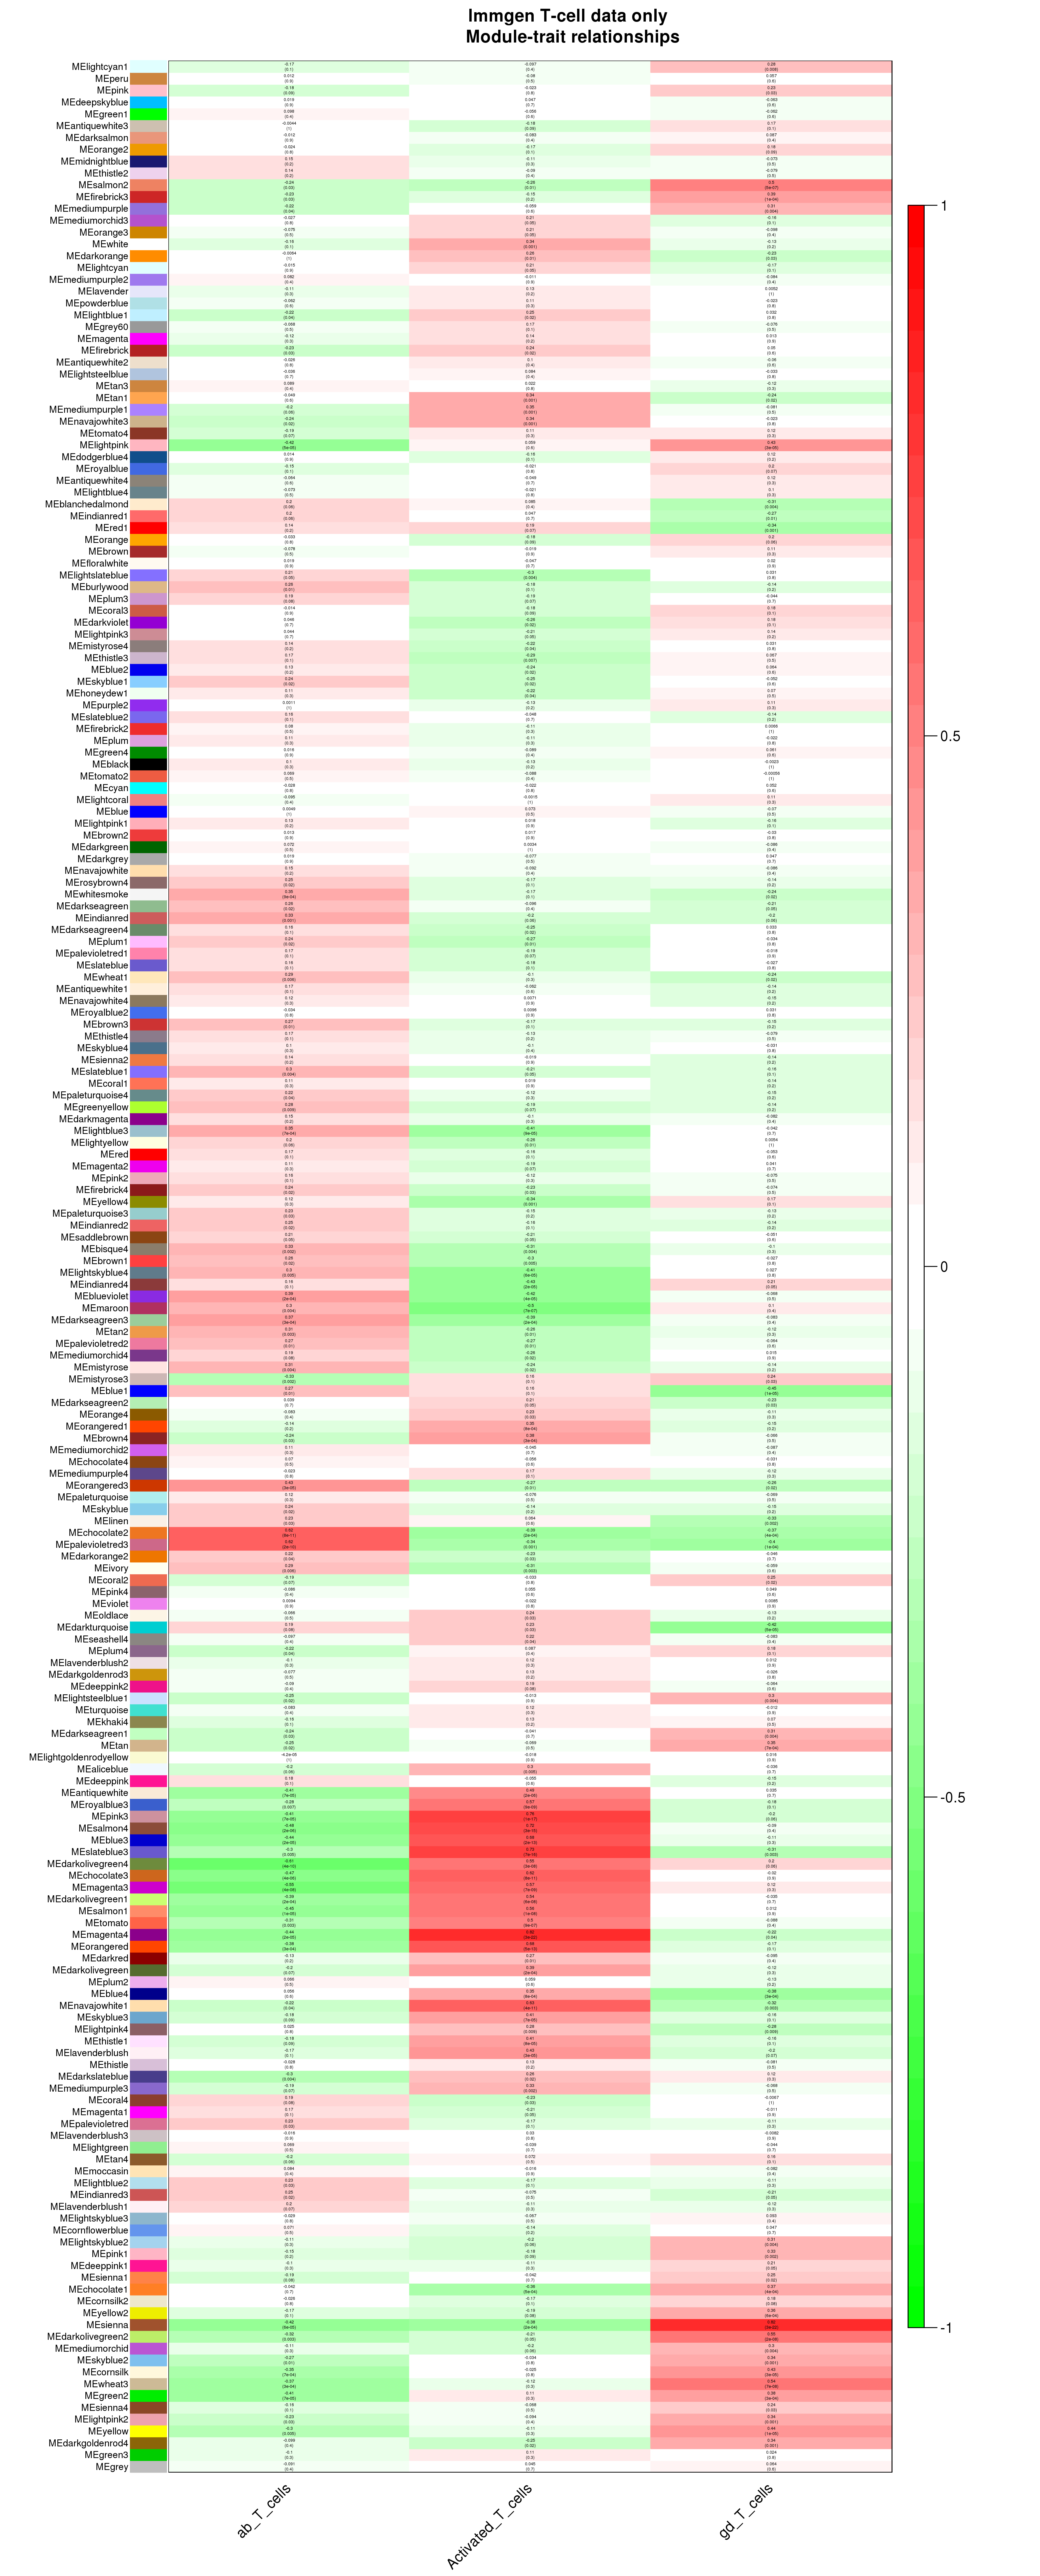
\includegraphics[width=0.58\textwidth]{Figures/Chapter4/WGCNA/tcell_immgen_data_module_trait_relationships_heatmap.png}
\caption{\small{Heatmap showing correlations between each of the WGCNA gene modules (y-axis) and the three T cell sub-populations. The colour bar to the right of the figure shows the colour coding scheme where strongly positive correlations are coloured red, strongly negative correlations are coloured green} }
    \label{fig:15}
\end{figure}

\section{Distribution of ImmGen Coarse module genes within T cell WGCNA clusters}

Table 4.1 below details how the genes within the 81 Coarse modules defined by ImmGen are distributed within the gene modules produced by reclustering the T cell data using WGCNA. The striking feature of of this table is that virtually all of the original modules defined by the ImmGen consortium have been split over multiple modules in the reclustering process. This could suggest one of two things. It may be that the observed differences in cluster solutions are simply a result of the fact that the intricacies of the algorithms used by WGCNA and PMC are quite different, WGCNA, as its name suggests, partitions data based on correlation strength while PMC does not incorporate this property of the data when clustering. Alternatively, the fact that this WGCNA analysis was performed using only T cell samples is likely to result in quite different clustering output than a more heterogeneous dataset. When the distribution of the WGCNA modules is compared to the ImmGen assignments, there do appear to be some broad similarities between the number of WGCNA modules genes of a given ImmGen Coarse module are split into and the number of Fine-grained modules reported by ImmGen. It is thus tempting to ponder whether the WGCNA modules determined in this analysis may in fact be more comparable to the ImmGen Fine modules. Whilst this could easily be quantified, we would not truly be be comparing like for like given that the ImmGen Fine modules were produced by reclustering of Course module data rather than from the expression dataset as a whole ~\autocite{Joj2013}.  

As discussed in Chapter \ref{Chapter3} only one of the Coarse modules published by ImmGen, C18, was T cell specific and was found to be comprised of genes whose functions relate to T cell activation. Given the group of WGCNA modules showing high positive correlations with the "Activated T cells" trait, we were particularly interested to determine whether there was any overlap between the genes assigned to these modules and those within Coarse module C18. The majority of genes comprising module C18 were not assigned to any of the WGCNA gene clusters analysed and hence it must be assumed that they were part of the large modules previously excluded from the WGCNA output module list. Of the C18 genes that were included in the final list of WGCNA modules, four out of a total of twelve modules showed significant correlation to the "Activated T cells" trait. These modules are: skyblue3 (\textit{p}-value = 7e\textsuperscript{-05}), thistle1 (\textit{p}-value = 8e\textsuperscript{-05}), darkslateblue (\textit{p}-value = 0.02), aliceblue (\textit{p}-value = 0.005). These modules vary in size between 16 and 56 genes which places them within the parameters of modules that are of appropriate scale to be of interest from a biological standpoint.  It is concerning however that most of the C18 genes were "lost" during WGCNA reclustering. 

\begin{landscape}
\small 
\begin{longtable}{|p{1.5cm}|p{1.25cm}|p{21cm}|}
\caption{Table detailing how genes assigned to each ImmGen Coarse module are dispersed within the modules generated by re-clustering of T cell samples with WGCNA}\\
\hline
ImmGen Coarse mod & Coarse mod size & Distribution of genes among WGCNA T cell data modules \\
\hline
1 & 334 & mediumpurple1 (6) darkred (50) salmon1 (2) darkolivegreen (22) thistle1 (7) deeppink (2) plum2 (15) lightsteelblue (4) darkolivegreen4 (2) lightpink4 (4) ivory (6) paleturquoise (2) tan4 (2) darkseagreen2 (2) skyblue (3) blue4 (4) lavenderblush1 (2) tan3 (5) brown (2) darkslateblue (2) greenyellow (5) navajowhite1 (2) white (2) yellow (2) skyblue3 (2) floralwhite (2) orangered (2) aliceblue (2) \\
2 & 229 & brown (23) floralwhite (21) orange (2) lightsteelblue (21) grey60 (14) antiquewhite2 (3) tan3 (2) black (4) darkred (2) lightskyblue4 (2) white (3) navajowhite3 (3) darkgreen (3) greenyellow (2) burlywood (2) brown1 (2) mediumpurple1 (7) lightcyan (3) lightslateblue (4) mistyrose (2) plum3 (2) tan1 (4) blue (4) darkorange (4) orangered3 (2) \\
3 & 344 & magenta (24) floralwhite (6) lightcoral (51) darkgrey (16) cyan (12) orangered1 (2) dodgerblue4 (4) royalblue (6) lightsteelblue (6) blue (16) brown2 (6) honeydew1 (2) lightpink3 (6) lightblue1 (7) black (4) grey60 (7) darkgreen (3) lightblue4 (5) darkviolet (2) antiquewhite2 (4) lightpink (5) indianred4 (2) brown (3) firebrick4 (2) antiquewhite4 (6) lightcyan (3) white (5) thistle3 (2) darkorange (2) \\
4 & 118 & skyblue4 (10) sienna2 (4) brown3 (3) slateblue1 (2) thistle4 (9) coral1 (4) lightblue1 (3) blue (3) lightcoral (4) dodgerblue4 (2) \\
5 & 313 & grey60 (27) darkorange (30) royalblue (5) orange3 (3) lightcyan (47) mediumpurple2 (3) cyan (3) blue (21) rosybrown4 (2) greenyellow (6) lightpink1 (9) darkseagreen3 (2) mediumorchid3 (4) floralwhite (13) bisque4 (5) lightsteelblue (4) black (5) darkgreen (6) white (7) lightcoral (3) mistyrose (2) magenta (4) brown (6) maroon (3) saddlebrown (2) indianred1 (3) lightblue1 (3) thistle3 (2) lightblue4 (2) \\
6 & 111 & lightcoral (5) magenta (13) lightcyan (6) grey60 (7) blue (14) antiquewhite4 (2) cyan (7) floralwhite (2) darkgrey (4) darkgreen (3) brown2 (2) mediumpurple2 (3) lightpink1 (2) slateblue (2) lightblue1 (3) brown (2) lightblue4 (3) plum (2) \\
7 & 30 & black (2) floralwhite (5) darkgreen (7) lightpink1 (3) \\
8 & 23 & floralwhite (3) antiquewhite4 (4) magenta (3) brown (2) \\
9 & 15 & blue (3) lightcyan (3) \\
10 & 14 & lightpink1 (3) blue (2) lightcyan (2) \\
11 & 153 & brown (91) orange (22) black (2) floralwhite (3) \\
12 & 46 & floralwhite (15) black (8) brown (14) \\
13 & 101 & honeydew1 (2) black (8) blue (8) floralwhite (12) lavender (3) maroon (5) cyan (2) darkgreen (3) plum3 (3) yellow4 (2) brown (2) plum1 (2) greenyellow (3) \\
14 & 73 & brown (34) floralwhite (21) blue (2) black (2) \\
15 & 38 & floralwhite (20) black (9) brown (3) \\
16 & 363 & blue (3) grey60 (3) thistle1 (3) violet (11) thistle (9) orangered3 (9) navajowhite1 (3) skyblue (18) darkslateblue (5) paleturquoise (10) darkorange2 (4) darkolivegreen4 (2) pink4 (2) coral2 (4) skyblue3 (11) black (2) mediumpurple3 (4) ivory (7) lightcyan (5) lightcoral (2) greenyellow (4) salmon2 (2) tomato (2) darkolivegreen1 (2) pink3 (2) palevioletred2 (2) lightpink1 (2) linen (3) white (2) yellow (2) salmon1 (2) palevioletred3 (3) magenta (2) \\
17 & 201 & thistle1 (15) lightpink2 (4) salmon4 (4) navajowhite1 (5) thistle (2) darkolivegreen (2) darkseagreen3 (2) lavenderblush (2) skyblue3 (7) brown (3) lightpink4 (5) darkslateblue (5) skyblue (4) coral2 (2) lightgreen (2) paleturquoise (3) mediumpurple3 (4) pink4 (4) violet (2) royalblue (2) saddlebrown (2) floralwhite (2) yellow (2) \\
18 & 146 & linen (3) orangered3 (8) skyblue3 (2) skyblue (4) darkgoldenrod4 (2) greenyellow (2) thistle1 (2) yellow (7) lightpink2 (5) darkslateblue (3) aliceblue (2) paleturquoise (2) \\
19 & 125 & darkmagenta (2) darkolivegreen1 (3) pink3 (3) yellow (14) sienna4 (3) brown4 (5) magenta4 (8) tomato (2) darkolivegreen4 (8) deeppink (4) chocolate3 (3) aliceblue (2) skyblue3 (2) midnightblue (2) salmon4 (2) skyblue2 (2) royalblue3 (3) orangered (5) wheat3 (2) lightskyblue3 (4) \\
20 & 54 & \\
21 & 82 & orangered1 (5) blue1 (2) darkolivegreen (3) darkseagreen2 (3) \\
22 & 39 & brown (4) darkred (5) darkseagreen2 (2) firebrick (2) lightsteelblue (2) tan3 (2) \\
23 & 54 & lightcoral (2) honeydew1 (2) lightsteelblue (2) darkgrey (2) floralwhite (6) blue (6) royalblue (3) cyan (3) grey60 (2) lightblue4 (3) \\
24 & 486 & blueviolet (2) lightgreen (10) midnightblue (13) magenta (5) red (21) lightyellow (9) saddlebrown (7) pink (27) thistle2 (4) darkolivegreen2 (3) coral3 (4) lightcoral (4) lightcyan (4) plum (6) yellow (24) mediumorchid4 (3) green3 (3) darkolivegreen4 (2) antiquewhite3 (2) lightsteelblue1 (4) darkmagenta (4) pink2 (3) honeydew1 (2) lightcyan1 (3) greenyellow (5) lavenderblush3 (3) coral4 (5) blue3 (2) tan4 (3) darkseagreen3 (2) mediumpurple (4) lightblue1 (3) yellow4 (3) floralwhite (2) brown4 (2) blue2 (3) sienna4 (2) blue (4) mediumorchid (3) thistle3 (3) \\
25 & 438 & pink (47) red (20) yellow (16) orangered (2) midnightblue (25) magenta4 (2) floralwhite (5) honeydew1 (2) darkolivegreen2 (6) lightskyblue3 (2) mediumorchid (10) blue (5) salmon4 (7) lightyellow (11) magenta1 (4) thistle2 (10) brown4 (3) skyblue2 (2) darkmagenta (2) indianred3 (2) palevioletred3 (2) tan4 (2) lightblue3 (2) orangered3 (2) royalblue3 (4) thistle1 (2) magenta2 (2) magenta3 (2) darkolivegreen4 (4) lightcyan1 (2) palevioletred (2) lightcoral (2) lightgreen (4) grey60 (2) \\
26 & 247 & lightcoral (2) red (6) thistle2 (3) lightcyan1 (3) yellow (6) lightgreen (4) lightyellow (8) mediumorchid (4) pink (3) saddlebrown (2) yellow4 (2) black (2) darkmagenta (2) maroon (2) green3 (2) \\
27 & 72 & plum3 (2) blue (2) greenyellow (2) brown4 (2) \\
28 & 55 & thistle2 (2) pink (3) red (4) midnightblue (3) lightsteelblue1 (2) brown4 (2) yellow (3) \\
29 & 37 & lightgreen (2) red (6) midnightblue (2) yellow (3) magenta1 (2) orange2 (2) antiquewhite3 (2) \\
30 & 76 & pink (16) red (3) darksalmon (2) darkgreen (2) midnightblue (2) lightgreen (3) thistle2 (2) \\
31 & 40 & pink (13) yellow (2) \\
32 & 101 & lightgreen (10) coral4 (10) yellow (5) magenta1 (2) brown4 (3) palevioletred (3) aliceblue (2) \\
33 & 147 & blueviolet (2) skyblue3 (2) greenyellow (3) plum4 (6) lightcyan1 (2) darkmagenta (2) red (4) lightgreen (3) mediumorchid (2) midnightblue (3) tan2 (2) thistle2 (3) black (2) pink (2) indianred4 (3) mediumorchid4 (3) \\
34 & 117 & skyblue3 (4) lavenderblush1 (3) yellow (5) thistle (4) mediumpurple3 (13) darkslateblue (2) chocolate4 (2) salmon1 (2) lightcoral (2) lightpink4 (2) navajowhite1 (2) \\
35 & 268 & deepskyblue (2) darkmagenta (2) lavenderblush3 (5) lightgreen (3) mistyrose (2) lightcyan1 (3) yellow (2) \\
36 & 202 & pink (2) brown4 (2) skyblue2 (2) yellow (3) darkmagenta (2) firebrick3 (2) lightcyan1 (2) deeppink1 (2) \\
37 & 41 & \\
38 & 42 & \\
39 & 45 & \\
40 & 67 & firebrick4 (2) thistle2 (4) yellow4 (2) midnightblue (5) lightyellow (3) red (3) lightgreen (2) lightskyblue3 (2) \\
41 & 54 & midnightblue (2) \\
42 & 53 & thistle2 (3) midnightblue (5) lightyellow (6) blue (4) red (7) honeydew1 (2) magenta2 (2) skyblue1 (2) \\
43 & 46 & lightyellow (2) midnightblue (4) red (6) indianred2 (2) lightblue2 (2) \\
44 & 118 & darkgrey (2) blue2 (2) skyblue2 (2) blue (2) yellow (3) firebrick2 (2) greenyellow (3) yellow4 (2) darkolivegreen2 (3) midnightblue (2) red (12) mediumorchid (3) black (2) firebrick3 (2) darkviolet (3) cyan (4) lightpink3 (2) lightcoral (2) thistle3 (3) \\
45 & 315 & maroon (2) floralwhite (5) salmon1 (2) slateblue3 (2) yellow (13) lightskyblue2 (3) lightsteelblue (4) lightgreen (4) navajowhite3 (2) chocolate3 (3) antiquewhite (4) darkolivegreen2 (2) darkolivegreen (6) royalblue3 (3) brown4 (2) midnightblue (2) navajowhite1 (3) salmon4 (3) magenta3 (6) darkolivegreen4 (5) darkolivegreen1 (3) pink3 (4) mediumpurple3 (3) red (4) brown (2) plum1 (2) darkred (2) tan4 (3) deeppink (2) mistyrose3 (2) aliceblue (2) thistle (2) orangered (3) \\
46 & 155 & yellow (5) lightcoral (14) coral1 (2) magenta (6) blue (4) cyan (7) darkgrey (6) black (2) royalblue (4) lightpink3 (3) darkgreen (3) lightcyan (2) cornsilk (2) brown (2) \\
47 & 134 & red (8) maroon (2) darkgreen (4) lightcyan (3) blue2 (5) floralwhite (5) indianred4 (11) blueviolet (5) firebrick4 (6) midnightblue (2) lavender (2) blue (4) magenta2 (4) black (8) lightyellow (6) honeydew1 (5) yellow4 (3) brown1 (2) greenyellow (2) grey60 (2) plum3 (2) indianred2 (2) \\
48 & 134 & darkslateblue (2) navajowhite1 (2) lightcyan1 (2) skyblue (5) greenyellow (4) palevioletred2 (2) floralwhite (2) darkolivegreen2 (2) yellow (5) paleturquoise (2) salmon4 (2) \\
49 & 108 & mistyrose4 (3) lightyellow (2) floralwhite (3) royalblue (5) thistle3 (2) black (3) red (3) lightsteelblue (3) honeydew1 (3) grey60 (3) brown (2) cyan (2) antiquewhite2 (2) lightcoral (3) \\
50 & 91 & plum1 (5) skyblue1 (2) saddlebrown (2) whitesmoke (2) darkviolet (2) midnightblue (2) floralwhite (3) blueviolet (5) red (5) blue (2) indianred4 (2) black (4) \\
51 & 51 & darkolivegreen (6) plum2 (4) darkred (9) mediumpurple1 (3) \\
52 & 149 & chocolate4 (11) mediumpurple4 (18) yellow (4) skyblue3 (6) skyblue (6) thistle (3) paleturquoise (9) brown4 (2) coral2 (3) navajowhite1 (2) mediumorchid2 (2) \\
53 & 97 & lightsteelblue1 (3) coral2 (3) yellow (7) paleturquoise (2) sienna4 (2) lightcyan1 (2) skyblue3 (2) salmon4 (2) lightgreen (2) mediumpurple3 (2) magenta3 (2) \\
54 & 38 & darkslateblue (4) skyblue3 (2) \\
55 & 26 & floralwhite (5) lightsteelblue (3) brown (4) \\
56 & 71 & cornflowerblue (6) salmon2 (12) lightcyan1 (4) pink1 (4) mediumpurple (2) lightyellow (2) deeppink (2) firebrick3 (2) \\
57 & 64 & greenyellow (17) palevioletred2 (7) chocolate1 (2) mistyrose (2) lightskyblue4 (2) tan2 (2) \\
58 & 55 & deeppink1 (2) pink (4) lightcyan1 (2) \\
59 & 15 & lightpink4 (3) \\
60 & 19 & firebrick3 (5) pink (2) \\
61 & 45 & darkgoldenrod4 (2) indianred3 (2) paleturquoise (2) yellow (2) skyblue3 (2) \\
62 & 62 & magenta3 (2) greenyellow (2) yellow (8) \\
63 & 37 & blue (2) \\
64 & 26 & yellow (2) darkslateblue (4) green3 (2) blue3 (2) \\
65 & 37 & yellow (25) \\
66 & 21 & lightsteelblue1 (2) \\
67 & 19 & paleturquoise (2) lightpink4 (2) skyblue3 (4) \\
68 & 14 & yellow2 (9) cornsilk2 (2) \\
69 & 22 & \\
70 & 13 & lavenderblush1 (2) \\
71 & 19 & yellow (2) saddlebrown (2) sienna4 (2) \\
72 & 13 & \\
73 & 12 & \\
74 & 15 & \\
75 & 12 & \\
76 & 15 & salmon2 (3) \\
77 & 11 & chocolate1 (2) \\
78 & 18 & greenyellow (2) \\
79 & 7 & \\
80 & 56 & yellow (2) pink (2) palevioletred1 (2) \\
81 & 211 & lightcyan (2) greenyellow (3) lightgreen (3) floralwhite (3) yellow (8) lightslateblue (2) pink (6) indianred3 (2) orange (2) moccasin (2) blue (2) lavenderblush3 (3) magenta4 (3) grey60 (2) lightsteelblue1 (3) brown (4) orange4 (2) \\
\hline
\end{longtable}
\end{landscape}

\section{Agglomerative Hierarchical clustering (Hclust)}

To provide a contrasting approach to the reclustering of the ImmGen T cell dataset with WGCNA, a hierarchical clustering algorithm was applied. Details of this methodology are provided in Chapter \ref{3}, but in summary the dataset was put through a two stage analysis whereby a correlation matrix was initially created using the "Person" method to calculate correlations between the expression profiles of all genes, before this correlation matrix was partitioned into clusters using Ward's method to measure the dissimilarity between observations. The output of this initial clustering was the dendrogram depicted in Figure 4.6. In contrast to WGCNA and other clustering algorithms, hierarchical clustering of a dataset is dependent upon manual specification of the desired number of clusters into which data should be split. To make this decision it is naturally necessary to make a visual inspection of the data and when analysing a significant number of genes, as was the case here, this can be problematic.  As Figure 4.6 and 4.7 show, even after two iterations it was not possible to determine the appropriate number of clusters between which to split the data and so the decision was made to iteratively partition the data into two clusters until such time as a greater number of separate, well-defined clusters were visible.

This technique is very time consuming and initially memory intensive, but it does afford the dubious advantage of being in complete control of the clustering process. Indeed, such a technique does hold an inherently higher risk of falling victim of human error but it is nevertheless still a popular choice for gene clustering analysis. One major challenge when performing hierarchical clustering on a dataset is that there is often no clear indication of when to stop partitioning the data and this could potentially result in meaningful gene clusters being either lost within a larger group, or perhaps more detrimentally being split between multiple modules. Both outcomes have the potential render the whole clustering process as effectively pointless. Following the careful and systematic clustering of the ImmGen T cell dataset, 443 modules were defined. This number is clearly much greater than in the previous analysis using WGCNA and indeed is almost incomparable to the original number published by ImmGen, which it should not be forgotten, included all immune cell types. Although the quality of the hierarchical clustering solution should naturally be assessed using measures outlined in Chapter \ref{Chapter1}, this drastic increase in the number of modules generated may suggest that the data may have been "over-clustered" resulting in many small gene modules which in reality are most likely to represent sub-modules. This is supported by the fact that although the modules produced ranged in size between 4 and 419 genes, over three quarters contained less than 100 genes and around half less than 50. Again however, it is important to stress that is a purely quantitative assessment and the qualitative analysis of these modules is still to be completed.  


\begin{figure}[H] 
    \centering
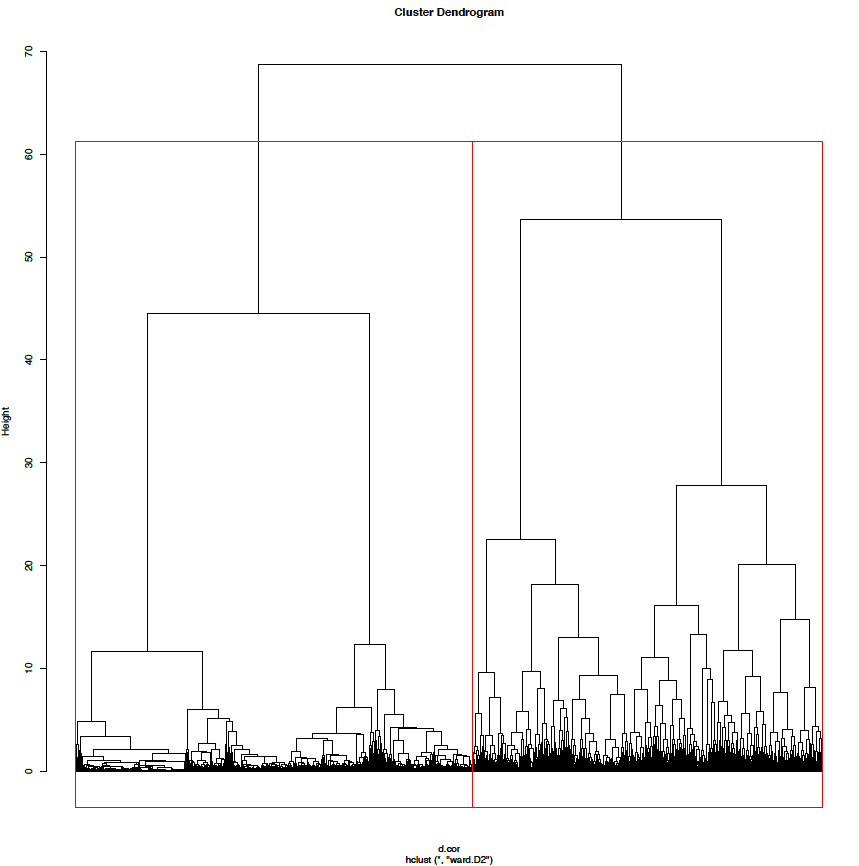
\includegraphics[width=0.9\textwidth]{Figures/Chapter4/hclust/immgen_tcell_only_hclust.png}
\caption{\small{Initial dendrogram resulting from hierarchical clustering of the ImmGen T cell dataset. Red borders separate the two clusters which will from the output of the first iteration (Clusters 1 and 2) } }
   \label{fig:16}
\end{figure}


\begin{figure}[H] 
    \centering
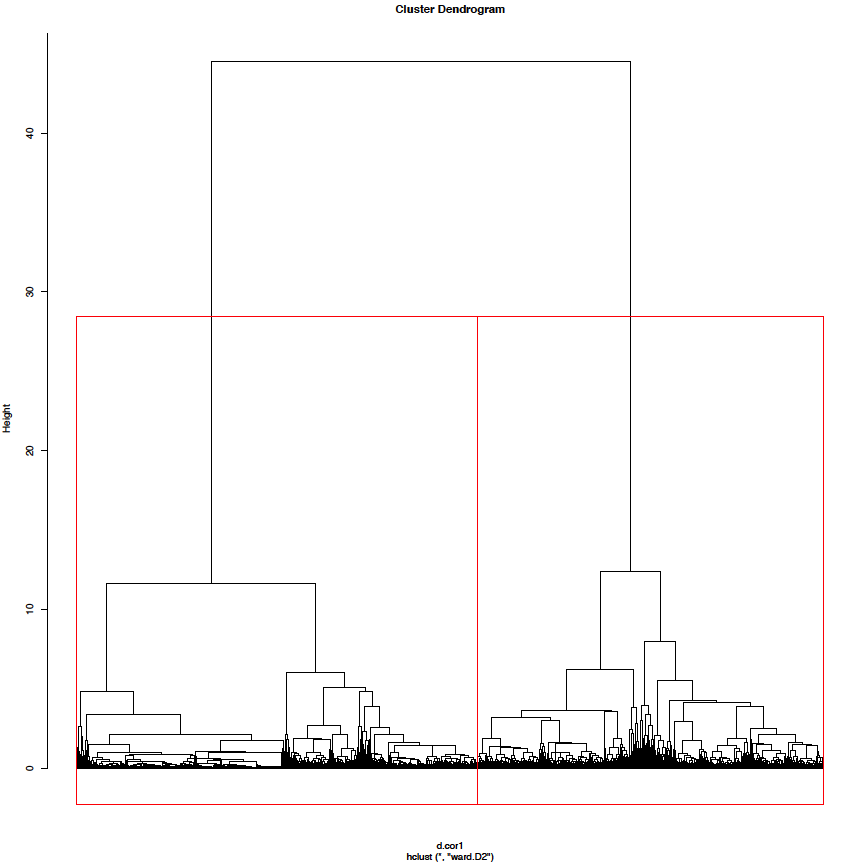
\includegraphics[width=0.9\textwidth]{Figures/Chapter4/hclust/immgen_tcell_only_hclust_CLUSTER1.png}
\caption{\small{Dendrogram depicting the result of hierarchical clustering of Cluster 1. Again, the data is partitioned into two clusters due to a lack of more detailed visual information regarding cluster separation. } }
\label{fig:17}
\end{figure}



\section{Distribution of ImmGen Coarse module genes within Tcell Hclust clusters}

Given the large number of gene modules produced by hierarchical clustering, it is perhaps unsurprising that when the distribution of genes among these clusters is compared to the ImmGen Coarse modules, the results are somewhat difficult to interpret from a biological perspective. Indeed, as can be seen from Table 4.2, when genes from a given ImmGen Coarse module are matched to a hierarchical clustering module, the overlap only extends to several genes at most. This is concerning as given that the ImmGen assignments all show at least a degree of cohesion in terms of functional annotation, the distribution of hierarchical clustering modules suggests that these properties have been lost during module partitioning. As both WGCNA and this form of hierarchical clustering separate observations based on correlations it would be interesting to directly compare their results to see how similar or otherwise the module assignments are.  

\begin{landscape}
\small 
\begin{longtable}{|p{1.5cm}|p{1.25cm}|p{21cm}|}
\caption{Table detailing how genes assigned to each ImmGen Coarse module are dispersed within the modules generated by re-clustering of T cell samples with Hclust}\\
\hline
ImmGen Coarse mod & Coarse mod size & Distribution of genes among Hclust T cell data modules \\
\hline
1 & 334 & 297 (2) 300 (2) 325 (2) 347 (2) 349 (3) 353 (2) 354 (3) 361 (3) 362 (6) 365 (4) 380 (11) 381 (4) 390 (27) 391 (7) 392 (5) 393 (33) 395 (4) 398 (8) 399 (9) 403 (2) 407 (3) 408 (3) 412 (2) 419 (22) 420 (8) 422 (17) 429 (3) 431 (2) 438 (23) 439 (12) 440 (6) \\
2 & 229 & 266 (2) 269 (2) 270 (10) 276 (2) 278 (2) 287 (2) 292 (3) 295 (2) 297 (4) 298 (4) 300 (3) 303 (14) 308 (2) 325 (8) 326 (5) 327 (3) 336 (2) 347 (3) 348 (6) 349 (12) 350 (6) 353 (4) 354 (5) 362 (4) 364 (2) 368 (2) 374 (4) 382 (2) 390 (6) 392 (5) 393 (7) 394 (2) 395 (3) 398 (4) 399 (2) 400 (3) 419 (8) 422 (3) 430 (2) \\
3 & 344 & 4 (2) 255 (2) 266 (4) 268 (8) 269 (4) 270 (3) 272 (9) 274 (4) 275 (12) 278 (4) 284 (4) 285 (2) 288 (5) 290 (4) 297 (23) 298 (15) 302 (4) 303 (17) 308 (2) 310 (2) 312 (8) 319 (5) 320 (7) 324 (2) 325 (2) 327 (7) 336 (2) 347 (5) 348 (3) 349 (21) 350 (2) 353 (24) 354 (15) 355 (3) 361 (2) 368 (2) 374 (2) 382 (3) 390 (6) 393 (4) 398 (3) 400 (3) 412 (2) 419 (4) 439 (2) \\
4 & 118 & 275 (2) 280 (2) 297 (2) 307 (2) 323 (12) 324 (5) 325 (2) 326 (3) 327 (2) 335 (6) 336 (5) 339 (9) 340 (2) 347 (2) 350 (5) 354 (2) \\
5 & 313 & 266 (3) 267 (6) 268 (2) 269 (2) 270 (3) 271 (2) 273 (13) 277 (3) 278 (2) 280 (4) 284 (5) 285 (6) 287 (3) 288 (2) 297 (8) 298 (31) 300 (5) 302 (2) 303 (7) 308 (18) 310 (2) 319 (2) 320 (7) 321 (5) 322 (14) 324 (4) 325 (4) 326 (2) 327 (4) 336 (3) 347 (2) 348 (2) 349 (9) 350 (2) 353 (19) 354 (13) 355 (2) 364 (2) 375 (2) 383 (2) 386 (2) 390 (5) 392 (3) 393 (3) 394 (3) 419 (2) 430 (2) 431 (3) 439 (4) 440 (2) \\
6 & 111 & 268 (3) 272 (2) 273 (3) 275 (5) 284 (2) 285 (3) 288 (3) 298 (9) 303 (4) 308 (4) 312 (6) 320 (5) 322 (3) 325 (2) 347 (2) 348 (3) 349 (2) 353 (16) 354 (7) \\
7 & 30 & 285 (2) 303 (2) 310 (2) 319 (4) 325 (4) 327 (5) \\
8 & 23 & 319 (2) 348 (2) 353 (5) \\
9 & 15 & 269 (2) 298 (2) 322 (3) \\
10 & 14 & 285 (3) 298 (2) \\
11 & 153 & 303 (2) 305 (33) 310 (5) 316 (8) 328 (6) 345 (3) 347 (8) 348 (6) 352 (35) 353 (8) 354 (5) 358 (4) 359 (3) \\
12 & 46 & 305 (8) 310 (4) 315 (2) 328 (3) 347 (3) 348 (4) 352 (9) 353 (6) 354 (2) \\
13 & 101 & 268 (3) 269 (2) 300 (2) 303 (6) 310 (2) 319 (4) 322 (2) 324 (2) 325 (3) 327 (7) 348 (5) 349 (2) 350 (2) 353 (6) 354 (3) 373 (2) 385 (3) 398 (3) 400 (5) 419 (2) 423 (3) 439 (2) \\
14 & 73 & 292 (4) 303 (5) 305 (4) 310 (7) 325 (2) 326 (2) 347 (3) 348 (8) 352 (8) 353 (7) 354 (3) \\
15 & 38 & 292 (2) 303 (2) 305 (2) 310 (7) 316 (2) 327 (2) 347 (6) 353 (4) 354 (2) \\
16 & 363 & 287 (3) 293 (2) 298 (2) 303 (2) 306 (2) 324 (2) 347 (2) 348 (2) 349 (3) 354 (2) 361 (5) 362 (5) 363 (2) 377 (3) 384 (2) 385 (6) 387 (2) 390 (16) 391 (21) 392 (10) 393 (4) 394 (3) 398 (2) 399 (10) 400 (7) 403 (5) 404 (2) 419 (40) 420 (8) 421 (2) 422 (14) 428 (5) 429 (6) 430 (13) 433 (2) 434 (2) 439 (13) 440 (13) \\
17 & 201 & 270 (2) 283 (2) 306 (2) 307 (2) 347 (2) 361 (2) 363 (2) 390 (6) 391 (11) 392 (3) 394 (4) 399 (6) 419 (19) 420 (9) 421 (2) 422 (12) 423 (2) 429 (3) 439 (6) 440 (9) \\
18 & 146 & 301 (2) 355 (2) 361 (3) 364 (2) 370 (2) 378 (2) 385 (3) 390 (2) 391 (5) 398 (3) 399 (3) 400 (8) 401 (2) 404 (2) 408 (2) 417 (2) 419 (4) 420 (6) 421 (3) 422 (4) 423 (3) 430 (11) 432 (2) 433 (2) 439 (5) 440 (5) \\
19 & 125 & 311 (4) 347 (3) 369 (3) 391 (2) 395 (4) 399 (2) 401 (14) 403 (16) 404 (8) 406 (4) 412 (2) 413 (5) 420 (5) 421 (4) 429 (6) 432 (5) 433 (3) 434 (2) \\
20 & 54 & 314 (6) 323 (2) 329 (6) 332 (2) 335 (2) 340 (2) 347 (3) 350 (2) 353 (10) \\
21 & 82 & 347 (3) 348 (2) 361 (4) 362 (2) 365 (2) 380 (4) 382 (2) 390 (5) 393 (6) 395 (6) 398 (6) 399 (2) 407 (6) 408 (2) 419 (2) 422 (2) \\
22 & 39 & 270 (2) 349 (2) 362 (2) 374 (3) 390 (4) 393 (5) 398 (2) 399 (3) 407 (2) \\
23 & 54 & 272 (2) 275 (2) 288 (2) 290 (2) 298 (3) 312 (2) 319 (4) 325 (3) 347 (2) 348 (2) 349 (2) 350 (2) 353 (4) 354 (2) \\
24 & 486 & 6 (4) 18 (3) 19 (3) 37 (3) 40 (2) 41 (2) 42 (2) 43 (3) 45 (3) 46 (4) 48 (2) 53 (2) 75 (4) 103 (2) 105 (2) 106 (2) 113 (2) 123 (3) 126 (3) 128 (2) 132 (3) 147 (2) 159 (2) 167 (2) 173 (2) 178 (2) 185 (2) 235 (2) 271 (2) 297 (8) 302 (4) 304 (3) 306 (3) 326 (2) 347 (13) 348 (16) 349 (16) 350 (8) 353 (2) 355 (20) 361 (4) 362 (5) 363 (9) 364 (2) 369 (5) 371 (4) 376 (2) 384 (2) 387 (2) 390 (3) 391 (7) 392 (8) 393 (3) 394 (3) 395 (18) 396 (4) 397 (6) 398 (8) 399 (17) 400 (6) 401 (10) 402 (4) 405 (4) 407 (3) 408 (6) 411 (6) 413 (6) 415 (2) 419 (2) 421 (2) 429 (7) 430 (3) 431 (3) 432 (3) 439 (5) \\
25 & 438 & 2 (3) 8 (3) 9 (2) 18 (2) 37 (2) 39 (2) 40 (2) 43 (2) 45 (3) 46 (2) 54 (2) 75 (2) 102 (2) 108 (2) 115 (2) 168 (2) 185 (2) 235 (3) 271 (2) 299 (6) 304 (2) 305 (2) 306 (2) 311 (2) 319 (2) 347 (34) 348 (9) 349 (8) 353 (2) 354 (3) 355 (24) 361 (2) 362 (2) 363 (2) 369 (2) 371 (6) 378 (3) 383 (2) 384 (2) 386 (3) 390 (7) 391 (3) 392 (3) 394 (3) 395 (10) 397 (7) 398 (3) 399 (6) 400 (5) 401 (7) 402 (5) 403 (9) 404 (3) 405 (4) 406 (4) 407 (2) 408 (8) 410 (9) 411 (8) 412 (2) 413 (12) 415 (5) 419 (4) 420 (4) 421 (3) 422 (2) 429 (14) 432 (4) \\
26 & 247 & 1 (4) 2 (3) 3 (5) 6 (2) 8 (2) 9 (2) 19 (2) 38 (2) 40 (4) 42 (4) 43 (3) 44 (3) 53 (3) 61 (2) 63 (2) 75 (2) 102 (2) 105 (2) 107 (2) 130 (2) 147 (2) 149 (3) 154 (2) 160 (2) 162 (2) 167 (5) 174 (2) 176 (4) 347 (13) 348 (6) 349 (2) 355 (4) 366 (2) 369 (2) 370 (2) 390 (3) 392 (2) 395 (7) 396 (2) 397 (2) 398 (2) 399 (6) 400 (2) 406 (2) 408 (2) 413 (2) 429 (5) \\
27 & 72 & 37 (2) 54 (2) 228 (2) 297 (2) 347 (4) 390 (2) 399 (2) \\
28 & 55 & 178 (2) 347 (9) 348 (3) 349 (2) 395 (3) 399 (2) \\
29 & 37 & 299 (2) 349 (4) 355 (4) 395 (2) 401 (2) \\
30 & 76 & 6 (2) 113 (2) 124 (2) 128 (3) 150 (2) 347 (4) 349 (3) 355 (4) 395 (2) 399 (2) 408 (3) 410 (2) 411 (4) 412 (2) 413 (2) 419 (2) \\
31 & 40 & 39 (2) 43 (2) 57 (2) 60 (2) 179 (2) 402 (3) 411 (2) 413 (4) 414 (2) \\
32 & 101 & 40 (2) 317 (3) 324 (2) 347 (2) 348 (2) 361 (2) 362 (2) 377 (2) 387 (5) 395 (3) 397 (3) 399 (5) 400 (3) 404 (2) 419 (2) 424 (5) 429 (13) 432 (2) \\
33 & 147 & 3 (3) 6 (2) 18 (2) 27 (2) 28 (2) 29 (2) 44 (2) 114 (5) 121 (3) 123 (2) 133 (3) 301 (2) 348 (3) 349 (5) 355 (4) 362 (3) 368 (2) 394 (2) 395 (5) 396 (3) 397 (2) 398 (2) 399 (3) 400 (3) 409 (3) 419 (2) \\
34 & 117 & 198 (2) 361 (3) 369 (3) 390 (3) 391 (5) 393 (2) 395 (3) 398 (4) 399 (5) 404 (2) 412 (2) 419 (6) 420 (4) 421 (4) 422 (5) 428 (2) 429 (8) 430 (2) 434 (2) 440 (5) \\
35 & 268 & 1 (2) 3 (5) 4 (2) 9 (2) 18 (3) 21 (3) 23 (2) 30 (2) 37 (7) 38 (6) 39 (4) 40 (5) 41 (2) 42 (4) 43 (4) 44 (4) 52 (3) 54 (3) 58 (2) 59 (2) 63 (3) 66 (2) 97 (2) 98 (3) 100 (2) 101 (5) 106 (3) 108 (2) 111 (3) 121 (2) 123 (6) 124 (8) 129 (2) 145 (7) 146 (3) 149 (2) 150 (2) 151 (2) 154 (4) 158 (4) 160 (3) 163 (2) 165 (2) 167 (5) 173 (6) 174 (3) 175 (4) 176 (2) 182 (2) 183 (2) 184 (2) 185 (3) 231 (4) 233 (2) 234 (2) 347 (5) 395 (6) 398 (2) 399 (2) 406 (2) 408 (3) 414 (2) \\
36 & 202 & 1 (2) 3 (5) 4 (3) 9 (3) 16 (2) 37 (6) 40 (7) 41 (4) 42 (5) 43 (5) 44 (6) 54 (3) 55 (2) 56 (2) 57 (2) 59 (4) 60 (2) 67 (2) 76 (2) 96 (4) 105 (3) 111 (2) 121 (4) 123 (3) 124 (5) 128 (2) 131 (3) 145 (2) 150 (4) 153 (2) 158 (3) 162 (2) 163 (2) 164 (2) 167 (2) 173 (4) 174 (3) 175 (2) 181 (2) 184 (3) 213 (2) 232 (2) 233 (2) 238 (2) 347 (3) 395 (2) 406 (2) 412 (2) 413 (2) \\
37 & 41 & 4 (2) 41 (4) 43 (4) 123 (2) 145 (2) 158 (2) \\
38 & 42 & 6 (3) 8 (2) 40 (5) 116 (2) \\
39 & 45 & 40 (2) 42 (3) 54 (2) 105 (2) 124 (3) 145 (2) 154 (2) 158 (2) 174 (2) \\
40 & 67 & 1 (2) 40 (2) 46 (2) 51 (2) 63 (2) 111 (2) 128 (2) 129 (2) 347 (9) 355 (6) 395 (2) 406 (2) \\
41 & 54 & 3 (3) 6 (3) 37 (3) 40 (2) 44 (2) 124 (2) 347 (2) 400 (2) \\
42 & 53 & 299 (2) 304 (3) 308 (2) 347 (10) 348 (4) 349 (3) 354 (2) 355 (9) \\
43 & 46 & 347 (10) 348 (2) 355 (6) 407 (2) 431 (2) \\
44 & 118 & 2 (2) 45 (2) 48 (3) 183 (2) 297 (3) 319 (2) 324 (2) 347 (4) 348 (10) 349 (4) 350 (4) 355 (5) 395 (2) 398 (3) 400 (3) 401 (3) \\
45 & 315 & 270 (2) 280 (2) 289 (2) 300 (3) 303 (2) 330 (2) 347 (5) 348 (6) 349 (9) 350 (3) 355 (2) 361 (8) 362 (5) 363 (2) 367 (3) 368 (4) 369 (8) 374 (2) 376 (3) 380 (3) 381 (2) 382 (3) 384 (2) 390 (13) 391 (15) 392 (6) 393 (6) 395 (5) 397 (3) 398 (10) 399 (15) 400 (9) 403 (4) 404 (5) 406 (3) 407 (2) 412 (2) 419 (6) 420 (14) 421 (5) 422 (4) 429 (14) 439 (2) 440 (5) \\
46 & 155 & 89 (2) 266 (3) 269 (5) 276 (3) 278 (4) 280 (2) 284 (2) 297 (2) 302 (4) 303 (3) 308 (3) 319 (2) 324 (2) 325 (4) 326 (4) 348 (4) 349 (6) 350 (2) 353 (5) 354 (5) 362 (6) 371 (3) 376 (3) 390 (4) 391 (2) 395 (4) 398 (2) 399 (3) 401 (2) 419 (2) \\
47 & 134 & 299 (4) 301 (4) 304 (2) 306 (2) 310 (2) 315 (2) 319 (2) 347 (19) 348 (10) 349 (4) 353 (2) 354 (9) 355 (17) 364 (2) 398 (4) 400 (3) 409 (2) 419 (3) \\
48 & 134 & 353 (2) 355 (2) 361 (8) 362 (3) 364 (2) 375 (3) 377 (2) 387 (2) 390 (7) 391 (6) 392 (3) 395 (3) 398 (4) 399 (2) 400 (5) 401 (2) 403 (5) 404 (3) 406 (2) 407 (3) 419 (4) 420 (2) 430 (2) 431 (3) 432 (2) 439 (3) \\
49 & 108 & 39 (2) 266 (2) 276 (2) 297 (5) 298 (2) 303 (3) 306 (3) 324 (3) 347 (3) 348 (3) 349 (3) 350 (4) 354 (3) 355 (3) 362 (2) 366 (3) 368 (2) 370 (2) 390 (6) 392 (2) 395 (2) 398 (3) 400 (2) \\
50 & 91 & 48 (2) 297 (2) 301 (2) 347 (7) 348 (6) 349 (3) 350 (5) 355 (6) 382 (2) 390 (2) 392 (2) 398 (6) 399 (3) 400 (3) \\
51 & 51 & 361 (4) 374 (2) 380 (5) 381 (2) 390 (4) 391 (3) 393 (4) 395 (2) 398 (2) 419 (3) 420 (4) \\
52 & 149 & 291 (3) 307 (10) 347 (3) 350 (4) 353 (4) 377 (2) 390 (5) 391 (4) 392 (3) 398 (4) 399 (5) 419 (10) 420 (3) 422 (9) 428 (2) 429 (3) 430 (6) 434 (2) 439 (4) 440 (4) \\
53 & 97 & 132 (2) 361 (2) 391 (2) 392 (7) 395 (5) 397 (2) 399 (2) 401 (2) 419 (10) 420 (2) 422 (2) 429 (6) 430 (2) 439 (4) 440 (2) \\
54 & 38 & 369 (2) 390 (3) 391 (3) 399 (2) 420 (3) 422 (3) 429 (2) 440 (5) \\
55 & 26 & 347 (4) 348 (3) 349 (2) \\
56 & 71 & 297 (2) 301 (12) 329 (2) 348 (4) 395 (3) 396 (2) 400 (2) 401 (7) 413 (2) 429 (2) 430 (2) \\
57 & 64 & 348 (2) 398 (4) 400 (6) 409 (5) 412 (2) 419 (2) 431 (15) \\
58 & 55 & 4 (3) 37 (2) 43 (3) 55 (2) 100 (2) 121 (2) 130 (2) 401 (2) 406 (2) 412 (2) \\
59 & 15 & 361 (2) 378 (2) 395 (2) \\
60 & 19 & 9 (2) 47 (2) 402 (2) \\
61 & 45 & 378 (2) 391 (5) 396 (2) 400 (4) 419 (2) 430 (3) 440 (3) \\
62 & 62 & 349 (2) 369 (2) 371 (2) 377 (2) 395 (4) 398 (2) 401 (3) 403 (4) 406 (2) 419 (2) 429 (2) \\
63 & 37 & 297 (2) 306 (2) 319 (2) 355 (2) 384 (2) 392 (4) 401 (2) 419 (5) \\
64 & 26 & 367 (2) 391 (4) 399 (2) 429 (2) \\
65 & 37 & 401 (7) 414 (4) 421 (2) 432 (10) \\
66 & 21 & 59 (2) 60 (2) \\
67 & 19 & 391 (3) 419 (4) 440 (2) \\
68 & 14 & 371 (3) 429 (4) \\
69 & 22 & 7 (4) 11 (2) \\
70 & 13 & 416 (2) 430 (2) \\
71 & 19 & 401 (2) 403 (6) 432 (2) \\
72 & 13 & \\
73 & 12 & \\
74 & 15 & \\
75 & 12 & 385 (2) 419 (3) \\
76 & 15 & 348 (2) \\
77 & 11 & 375 (2) \\
78 & 18 & 390 (2) 399 (2) 408 (2) 431 (2) \\
79 & 7 & \\
80 & 56 & 44 (2) 162 (2) 341 (2) 361 (2) 398 (2) 410 (2) \\
81 & 211 & 1 (2) 6 (3) 8 (2) 11 (2) 42 (3) 43 (3) 103 (4) 114 (5) 133 (2) 173 (2) 174 (2) 347 (2) 348 (3) 349 (2) 353 (4) 354 (2) 361 (2) 365 (2) 370 (2) 390 (3) 395 (3) 398 (5) 399 (2) 400 (3) 401 (2) 403 (3) 405 (2) 408 (2) 411 (3) 420 (2) 429 (2) 432 (2) 434 (2) \\
\hline
\end{longtable}
\end{landscape}

\section{K-means}

The two methods utilised in the above re-clustering analyses of the T cell data both rely on measurement of the correlations between gene expression profiles to act as the clustering metric. Whilst this may seem like logical approach when dealing with expression data, there are alternatives. With this in mind, the decision was made to perform a third analysis using K-means which does not take account of correlation values between observation. It was hoped that this would provide a means by which the relative importance of the use of correlations as a key component of gene clustering could be quantified to some extent. Unlike either WGCNA or H-clust it is necessary to define the number of clusters between which observations will be split before K-means can be run. The best technique used to determine K is the subject of much debate and this process often involves a degree of trial and error. One of the most popular methods to determine K is the "Elbow" method, described in Chapter \ref{Chapter3}, and the plot displayed in a figure 4.8 represents how the variance within the dataset decreases as the number of clusters K increases. As is evident from this plot, this algorithm produces a very different clustering solution for the T cell data set when compared to WGCNA or hierarchical clustering. Indeed, using the "Elbow" plot depicted in figure 4.8 to choose a value for \textit{k} where the greatest proportion of variance is explained within as few clusters as possible results in 9 gene clusters/modules being produced. Of these 9 modules, one contained over 13000 genes and as such was designated as a "bin" module and therefore was removed from further analysis. The remaining modules range in size from 6 to 4506 genes which, given the small number of modules in total, is quite a surprisingly large variation. If these module assignments were to be believed, it would suggest that this dataset can only be segregated into a handful large groups as well as several very small ones. Given that the purpose of this re-clustering analysis is to identify modules which are likely to represent biologically relevant, cohesive gene groups, it seems that K-means is not a particularly appropriate algorithm to use. Instead, it seems to be favourable to take advantage of alternative clustering methods which are able to incorporate correlation values between genes when splitting the data set. 

\begin{figure}[H] 
    \centering
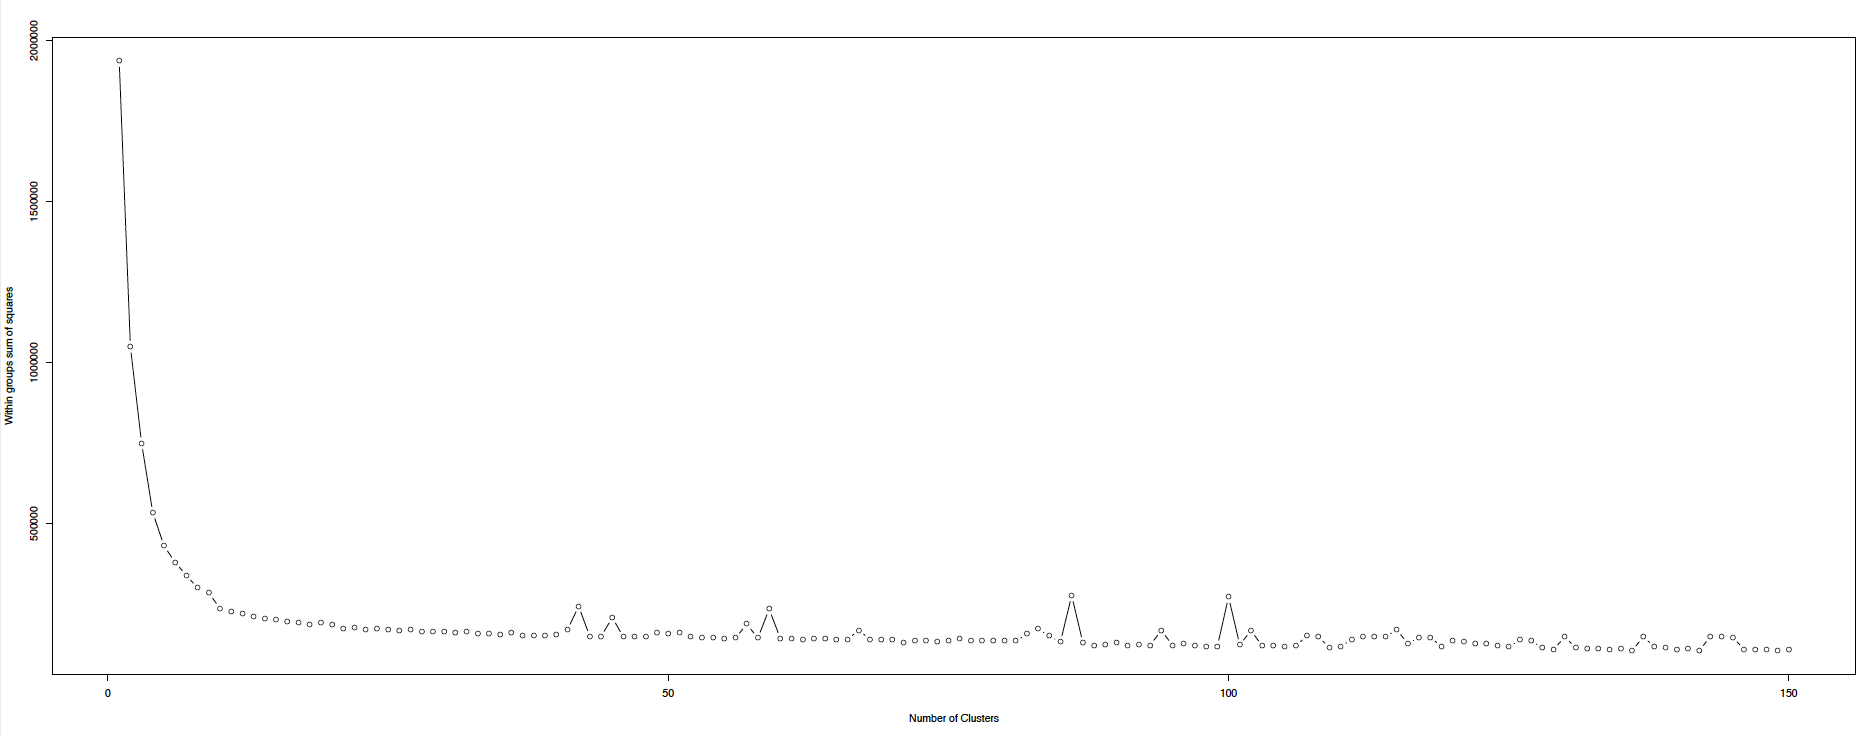
\includegraphics[width=0.95\textwidth]{Figures/Chapter4/kmeans/immgen_tcell_only_wssplot.png}
\caption{\small{An "elbow" plot showing how increasing the number of \textit{K} clusters results in a decrease in the overall within-module variance of the T cell data. The optimal value of \textit{K} is believed to sit at the point where adding additional clusters does not result in a substantial increase in the proportion of variance explained i.e. the "elbow" of the plot.} }
   \label{fig:18}
\end{figure}

\section{Distribution of ImmGen Coarse module genes within T cell K-means clusters}

For completeness we performed the same comparison of gene assignments between the ImmGen coarse modules and those produced by \textit{k}-means clustering, although given the small number of clusters resulting from the \textit{k}-means analysis, it is fair to say that this comparison is likely to be of limited value. Indeed, inspection of table 4.3 shows that \textit{k}-means module gene assignments are split across many of the ImmGen modules, providing further evidence that the clusters produced during the latest analysis of the T cell dataset do not represent modules of closely related gene expression profiles. It is possible that re-clustering of each \textit{k}-means module individually may result in better defined, more biologically relevant gene groups, but given that this algorithm clusters based purely on physical distances between data points, the results are unlikely to better those of more complex clustering methodologies such as WGCNA when it comes to the clustering of gene expression data.

\begin{landscape}
\small 
\begin{longtable}{|p{1.5cm}|p{1.25cm}|p{21cm}|}
\caption{Table detailing how genes assigned to each ImmGen Coarse module are dispersed within the modules generated by re-clustering of T cell samples with K-means}\\
\hline
ImmGen Coarse mod & Coarse mod size & Distribution of genes among K-means T cell data modules \\
\hline

1 & 334 & 2 (74) 7 (67) 4 (20) 3 (4) 1 (97) \\
2 & 229 & 3 (5) 2 (80) 1 (58) 7 (30) 4 (6) \\
3 & 344 & 7 (25) 2 (166) 3 (2) 1 (74) \\
4 & 118 & 3 (15) 2 (22) 4 (17) 6 (10) 7 (9) 1 (9) \\
5 & 313 & 2 (131) 1 (86) 7 (36) 3 (3) 4 (10) \\
6 & 111 & 7 (7) 1 (28) 2 (52) 4 (2) \\
7 & 30 & 2 (9) 1 (10) 4 (3) 7 (5) \\
8 & 23 & 1 (5) 2 (8) 4 (2) \\
9 & 15 & 1 (5) 2 (5) 7 (2) \\
10 & 14 & 1 (6) 7 (2) 2 (4) 4 (2) \\
11 & 153 & 1 (12) 2 (52) 7 (7) 8 (10) 4 (2) \\
12 & 46 & 2 (20) 1 (3) 7 (3) \\
13 & 101 & 2 (40) 7 (13) 1 (16) 4 (11) \\
14 & 73 & 2 (25) 7 (3) 1 (17) \\
15 & 38 & 2 (16) 7 (3) 1 (8) \\
16 & 363 & 2 (89) 1 (115) 7 (65) 4 (33) 3 (10) 6 (4) \\
17 & 201 & 1 (56) 3 (12) 4 (30) 7 (43) 6 (7) 2 (30) 5 (2) \\
18 & 146 & 7 (22) 2 (36) 1 (29) 4 (10) 3 (7) \\
19 & 125 & 1 (17) 2 (32) 3 (3) 4 (2) 7 (2) \\
20 & 54 & 3 (2) 1 (11) 2 (16) 7 (5) 6 (4) 4 (2) \\
21 & 82 & 2 (30) 7 (4) 1 (12) \\
22 & 39 & 2 (16) 1 (9) 7 (3) \\
23 & 54 & 7 (6) 2 (22) 1 (15) 4 (2) \\
24 & 486 & 2 (135) 1 (39) 7 (11) 4 (3) \\
25 & 438 & 2 (120) 1 (31) 7 (12) \\
26 & 247 & 1 (7) 2 (35) 7 (2) \\
27 & 72 & 2 (11) 1 (5) \\
28 & 55 & 1 (2) 2 (4) \\
29 & 37 & 2 (14) 1 (2) \\
30 & 76 & 2 (10) 1 (3) 7 (3) \\
31 & 40 & \\
32 & 101 & 2 (44) 1 (14) 7 (9) 4 (4) \\
33 & 147 & 2 (27) 7 (4) 1 (9) \\
34 & 117 & 1 (23) 2 (39) 4 (8) 7 (18) 3 (3) 6 (5) \\
35 & 268 & 2 (8) \\
36 & 202 & 2 (5) \\
37 & 41 & \\
38 & 42 & 2 (2) \\
39 & 45 & \\
40 & 67 & 2 (4) \\
41 & 54 & 2 (2) \\
42 & 53 & 2 (20) 1 (2) \\
43 & 46 & 2 (2) \\
44 & 118 & 7 (5) 2 (26) 1 (4) \\
45 & 315 & 2 (125) 1 (66) 7 (26) 4 (7) 3 (6) \\
46 & 155 & 2 (64) 1 (39) 4 (7) 7 (8) \\
47 & 134 & 2 (44) 7 (4) 1 (9) \\
48 & 134 & 7 (11) 2 (54) 1 (24) \\
49 & 108 & 2 (47) 1 (21) 7 (8) \\
50 & 91 & 2 (33) 1 (9) \\
51 & 51 & 2 (20) 1 (19) 4 (2) \\
52 & 149 & 4 (10) 7 (21) 2 (41) 1 (36) 3 (7) 6 (2) \\
53 & 97 & 1 (25) 2 (28) 7 (12) 4 (9) \\
54 & 38 & 2 (10) 4 (5) 1 (10) 7 (9) \\
55 & 26 & 2 (8) 1 (4) \\
56 & 71 & 2 (23) 1 (6) 4 (2) \\
57 & 64 & 2 (25) 1 (5) 7 (3) 4 (2) \\
58 & 55 & \\
59 & 15 & 2 (5) \\
60 & 19 & 2 (6) \\
61 & 45 & 2 (13) 1 (16) 7 (4) \\
62 & 62 & 2 (26) 1 (5) \\
63 & 37 & 1 (17) 2 (9) 7 (4) \\
64 & 26 & 1 (5) 2 (12) 3 (2) \\
65 & 37 & 2 (7) 1 (2) \\
66 & 21 & \\
67 & 19 & 1 (9) 7 (4) 2 (3) \\
68 & 14 & 2 (8) 1 (2) 7 (2) \\
69 & 22 & \\
70 & 13 & 2 (4) \\
71 & 19 & 2 (9) \\
72 & 13 & 2 (3) \\
73 & 12 & \\
74 & 15 & \\
75 & 12 & 1 (4) 2 (5) \\
76 & 15 & 2 (3) \\
77 & 11 & 2 (6) 1 (3) \\
78 & 18 & 1 (4) 2 (5) \\
79 & 7 & \\
80 & 56 & 2 (6) 6 (3) \\
81 & 211 & 7 (9) 1 (16) 2 (33) 3 (2) \\


\hline
\end{longtable}
\end{landscape}

\section{Conclusions and Future Work}

Here we present the results of re-clustering of T cell data from the publicly available ImmGen resource. WGCNA, Hclust and \textit{K}-means were all applied to this dataset with surprisingly varied results. Indeed, while WGCNA and Hclust produced many gene modules, \textit{K}-means clustering delivered only a handful. It is believed that this latter result is due to the fact that in \textit{K}-means clustering, no account is taken of the correlations between samples. In a biological context, correlation analysis is one of the key ways in which we can determine the relationship between genes in a given setting and so to ignore these connection seems rather counter intuitive. We therefore suggest that \textit{K}-means is not an appropriate choice for the clustering of large gene expression datasets. This work also highlights the need for the establishment of comprehensive and user-friendly module annotation and qualitative assessment techniques. Without these, it is not feasible to attempt detailed annotation of such large module lists and so we can not truly evaluate the above clustering results at this time.






\chapter{Quantitative analysis reveals epidermis-specific gene module: Evidence of T-cell reprogramming in GVHD target tissues?} % Main chapter title

\label{Chapter5} % For referencing the chapter elsewhere, use \ref{Chapter1} 

%----------------------------------------------------------------------------------------

\section{Overview}

In this Chapter we utilise our module-based refined testing protocol to survey the relative expression of the 31 WGCNA-derived MataHari gene modules in both the dermis and epidermis in the presence or absence of LCs. In this way we hoped to identify any modules which were both significantly associated with, and differentially expressed in, either the dermis or epidermis as well as evaluate how results obtained using our refined testing protocol compared to those produced by a more standard methodology, the Fisher's Exact Test. 

\section{Background - Depletion of Langerhans cells (LC) in the MataHari (Female $\to$ Male) model}

As mentioned in Chapter \ref{Chapter2}, once effector T cells have been activated and recruited to a specific tissue they will interact with various resident APC populations. In the skin this includes epidermal Langerhans cells (LC). It has been demonstrated that epidermal LCs are able to exert control over T cell activation ~\autocite{Igy2013} but whether they play an additional role in the pathogenic re-programming of effector T cells within tissues is currently unclear. If it was found that interactions between CD8$\textsuperscript{+}$ T cells and tissue resident LC populations did result in re-programming of the former population, this could help further our understanding of the specific events that culminate in target organ pathology in GVHD. 

To investigate the relationship between effector T cells and epidermal LCs we adapted our MataHari F $\to$ M BMT model to allow exploration of whether interaction with resident LCs was responsible for effector CD8$\textsuperscript{+}$ T cell reprogramming, particularly for inducing the epidermis-specific gene module, M28 that was identified during previous work with this GVHD mouse model (details in Chapter \ref{Chapter1}). Using Multi-photon imaging it was shown that seven days after BMT effector T cells migrating to the skin formed connections with radio-resistant, host-derived LCs in the epidermis, but no interactions with donor-derived cells were observed most probably due to low cell counts at this time point ~\autocite{Santos}. Depletion of host-derived LCs with diphtheria toxin ~\autocite{Ben2005,Kis2005} prior to BMT revealed that this population was required for the accumulation of effector T cells in the epidermis while the depletion of host-type dermal Langerin$+$ DCs had no effect ~\autocite{Santos}. A similar requirement for LCs in the process of CD8$\textsuperscript{+}$ T cell migration into the epidermis was also seen in the B6 into 129sv model. Although LCs are known to be highly motile ~\autocite{Kis2005}, experiments depleting LCs unilaterally in one ear of a mouse at the time of BMT resulted in loss of effector T cell populations in the manipulated ear only ~\autocite{Santos}. This finding supports the notion of the need for LCs \textit{in situ}. Interestingly, host-strain LC purified from allogeneic recipients compared to those undergoing syngeneic BMT showed high levels of enrichment for IFN-g-responsive genes. It is this group of genes that are also prevalent in the gene module M28 identified using the MataHari dataset. Additionally, when host IFN-$\gamma$ receptor signalling was blocked, LCs post allogeneic BMT failed to up-regulate MHC class I expression and CD8$\textsuperscript{+}$ T cell accumulation was reduced specifically in the epidermis but not within other tissues ~\autocite{Santos}.

\section{Analysis of MataHari WGCNA-derived gene modules with standard categorical association testing method} 

Having demonstrated a requirement for LCs in the successful migration and accumulation of effector T cells in the epidermal skin compartment, we hypothesised that any gene modules involved in establishment of an inflammatory environment should be highlighted by differential expression analysis of LC depleted versus LC replete populations. To investigate this theory we surveyed the relative expression of the 31 WGCNA-derived MataHari gene modules in both the dermis and epidermis in the presence or absence of LCs (using data from the LC depletion experiments mentioned in the previous section). For each of the differential expression datasets (dermal and epidermal) we applied both a standard Fisher's Exact Test as well as our module-based refined testing protocol. For any given gene module, by plotting the differential expression \textit{p}-value against the trait association \textit{p}-value obtained as part of the WGCNA analysis (Chapter \ref{Chapter3}) we hoped to identify any modules which were both significantly associated with, and differentially expressed in, the particular skin compartment being analysed. In the following sections we present the results of this analysis, focusing initially on data from effector T cells in the dermis and then turning to the epidermal population. Both association testing methodologies are described in detail in Chapter \ref{Chapter3}. 

\subsection{Analysis of dermal effector T cell populations} 

Figures 5.1 and 5.2 below plot the results of comparing the dermis WGCNA trait association \textit{p}-value for each module (the same values apply in both comparisons) against the differential expression \textit{p}-value obtained with Fisher's Exact Test and our own module-based refined test respectively. As can be seen from both plots, the MataHari modules do exhibit varying trait associations with the dermis which is unsurprising given the variety of functions there contain as a group (see Figure 1.5), but none are particularly strong statistically. When Fisher's Exact Test was applied to quantify the extent of modular differential expression changes following LC depletion, none of the gene modules were found to be significant. This would suggest that none of the MataHari modules contain substantially more genes differentially expressed in LC depleted versus control mice than any other. Turning to the results acquired when using our refined testing protocol to analyse the differential expression data from the LC depletion study (Figure 5.2), it is evident that we do indeed see enhanced significance of certain gene modules when overall direction of effect in terms of the up-/down-regulation of module genes is incorporated into the association testing methodology (for details see Chapter \ref{Chapter3}.2.3). Examination of Figure 5.3 reveals that three of the MataHari modules, namely M4, M17 and M23, show particularly enhanced association with the dermis in LC depleted mice compared to the values seen in Figure 5.1 when using Fisher's Exact Test in isolation. 

\begin{figure}[H] 
    \centering
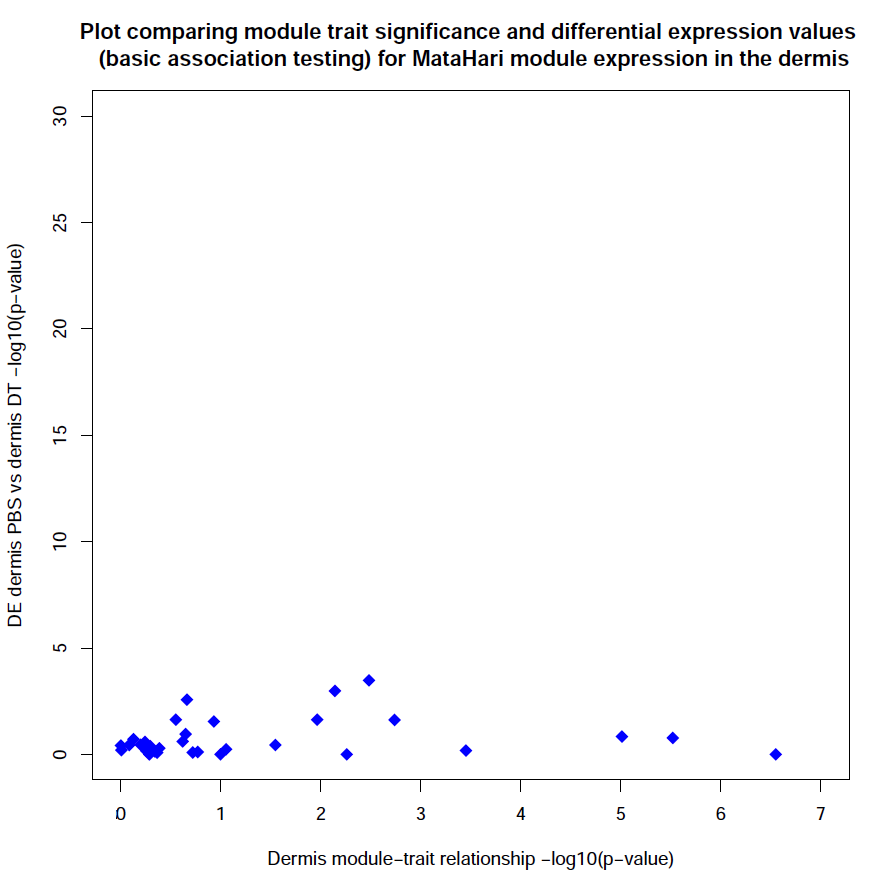
\includegraphics[width=0.6\textwidth]{Figures/Chapter5/Dermis_trait_vs_DE_BASIC.png}
\caption{\small{Graph of WGCNA-defined MataHari modules showing \textit{p}-values for correlation to dermis (x-axis) and differential expression association according to presence or absence of LC and quantified using Fisher's Exact Test (y-axis).} }
    \label{fig:23}
\end{figure}


\begin{figure}[H] 
    \centering
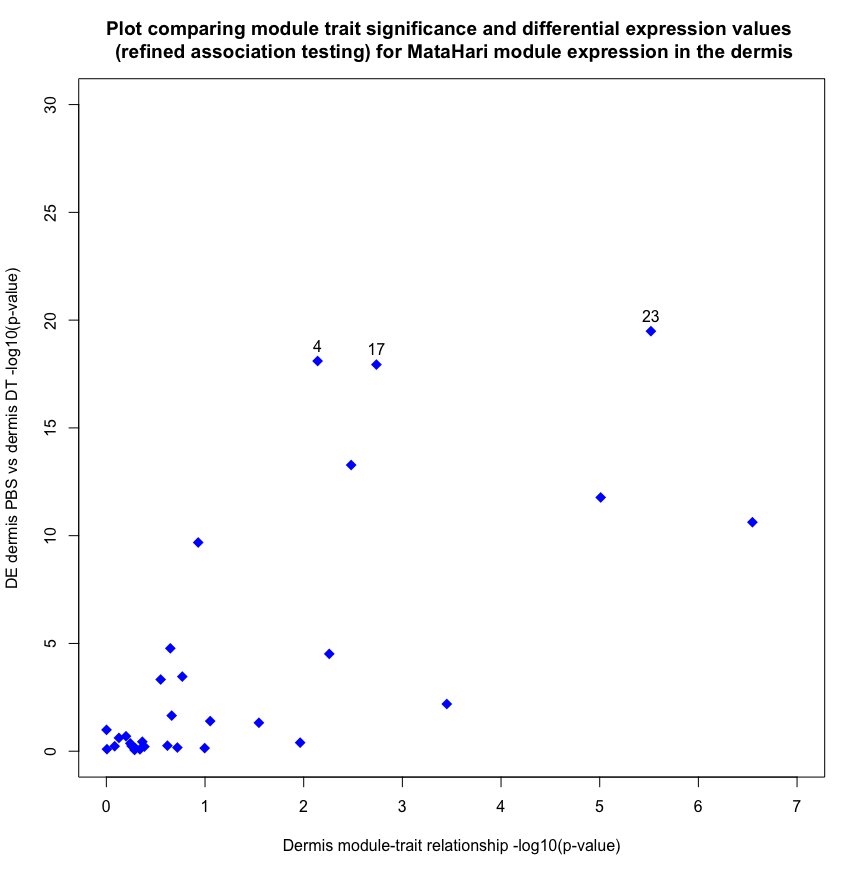
\includegraphics[width=0.6\textwidth]{Figures/Chapter5/Dermis_trait_vs_DE.png}
\caption{\small{Graph of WGCNA-defined MataHari modules showing \textit{p}-values for correlation to dermis (x-axis) and differential expression association according to presence or absence of LC and quantified using module-based refined test (y-axis).} }
    \label{fig:24}
\end{figure}

During previous work in the laboratory module based enrichment in Gene Ontology annotations were determined (Chapter \ref{Chapter3} for brief overview of WGCNA methodology) and these are summarised in Figure 1.5. Studying the annotations for M4, M17 and M23 the results are quite interesting when taken in the context of GVHD pathology. Module M4 represents a large collection of genes, many of which are involved in the key metabolic pathway responsible for ATP generation, oxidative phosphorylation ~\autocite{Santos}. The somewhat smaller gene module M17 is thought to be driven by genes encoding multiple Toll-like receptors which are known to play a key role in pathogen recognition and activation of innate immunity via the pathogen-associated molecular patterns (PAMPs) that are expressed on infectious agents ~\autocite{Santos}. These receptors also mediate the production of cytokines required for the development of effective immunity. Interestingly, the third gene module to show both significant differential expression and trait association with the dermis, M23, is comprised of many cytokine and cytokine receptor encoding genes ~\autocite{Santos}. As discussed in Chapter \ref{Chapter2}, cytokines modulate the balance between humoral and cell-based immune responses, and help regulate the maturation, proliferation and responsiveness of T cell populations. As summarised in Figure 1.5, expression of M17 and M23 was found to be enriched in the secondary lymphoid organs of allogeneic BMT recipients, while M23 was instead correlated with GVHD target organs in the same allogeneic recipient group ~\autocite{Santos}. Put together, these results indicate groups of differentially expressed genes showing association with the dermal skin compartment, in part highlighted through use of our refined testing protocol, that are known to be involved in modulating immune responses and cytokine activity. Thus by utilising modular direction of effect data we can enhance the sensitivity of differential expression based analysis, in this case highlighting changes in expression levels of inflammatory related genes when LCs are depleted in the dermis. 

\subsection{Analysis of epidermal effector T cell populations} 

Applying the same differential expression analyses in combination with WGCNA derived trait associations to epidermal data, we obtain the module association results depicted in Figures 5.3 and 5.4 below. 

\begin{figure}[H] 
    \centering
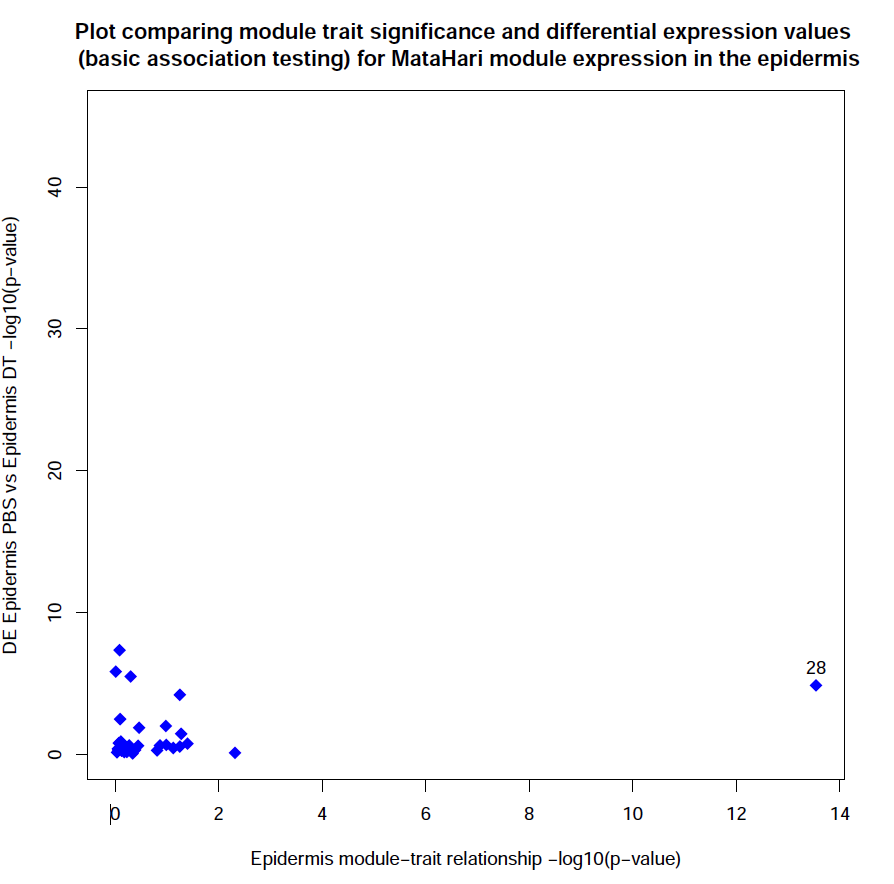
\includegraphics[width=0.5\textwidth]{Figures/Chapter5/Epidermis_trait_vs_DE_BASIC.png}
\caption{\small{Graph of WGCNA-defined MataHari modules showing \textit{p}-values for correlation to epidermis (x-axis) and differential expression association according to presence or absence of LC and quantified using Fisher's Exact Test (y-axis).} }
    \label{fig:25}
\end{figure}

As is clear from a comparison of Figures 5.1 and 5.3, there are notable differences between the relative significance of trait associations of the 31 MataHari gene modules in the dermis and epidermis. Whereas the modules showed a range of trait association values in the dermis data, they generally appear much more clustered at low significance values in the epidermis samples. That being said, the epidermis data reveals one marked exception, module M28. As evidenced by Figure 5.3, MataHari module M28 is strongly associated with the "dermis trait" and yet does not stand out in terms of differential expression significance. However, application of our module-based refined association test gives a very different picture. 

Figure 5.4 shows the difference made by including direction of effect data during the module association testing. Several of the MataHari modules now exhibit highly significant differential expression associations in the LC depletion dataset, with much stronger \textit{p}-values than seen in the dermis. What is more interesting however is that a substantial jump in significance is observable in the case of M28. As can be seen clearly in Figure 5.4, gene module M28 is unique in both the dermal and epidermal datasets as being significantly expressed in the epidermis and showing a very high level of differential expression in the presence or absence of LC (\textit{p}$<10^{-30}$). This effector T cell module was thus found to be highly specific for the epidermal compartment of the skin and as mentioned in Chapter \ref{Chapter1} contains genes relating to Interferon-$\gamma$ signalling including many pro-inflammatory cytokines (e.g. Ifng, Il2, Il3, Csf1 and Csf2), cytokine receptors and downstream adaptors (e.g. Il2ra, Il1r1, Il18rap) ~\autocite{Santos}.  Interferon-$\gamma$ is believed to be a primary driver gene for module M28 and follow-up experiments demonstrated the reduction of this genes mRNA and protein expression levels in LC depleted mice ~\autocite{Santos}. 

\begin{figure}[H] 
    \centering
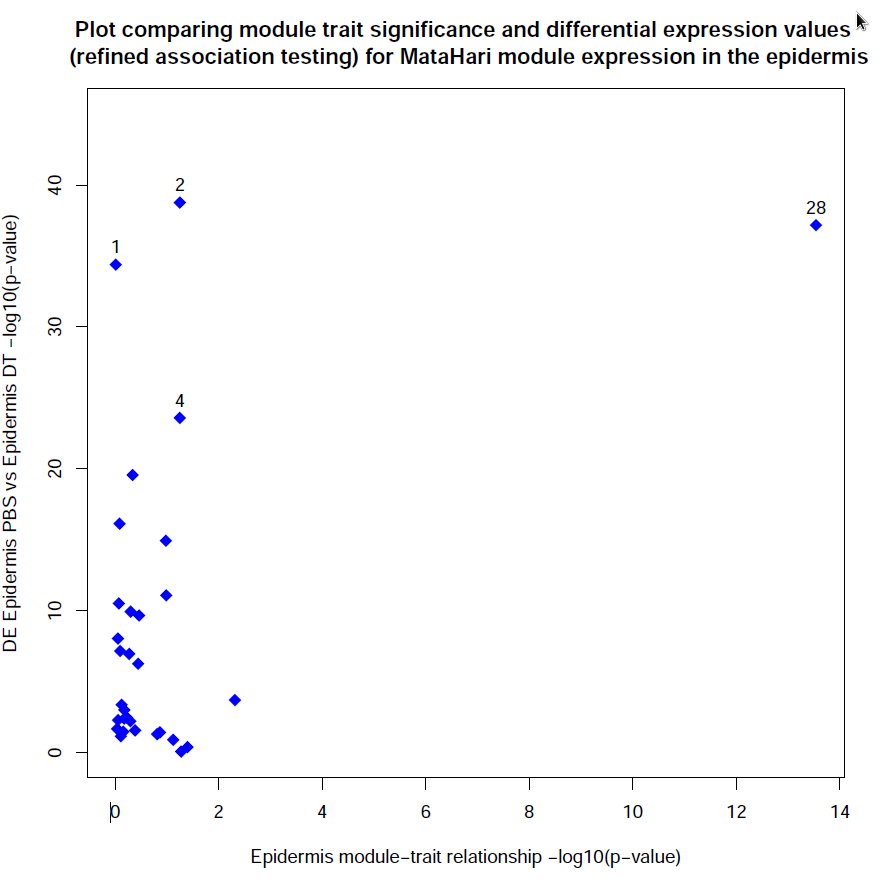
\includegraphics[width=0.6\textwidth]{Figures/Chapter5/Epidermis_trait_vs_DE.png}
    \label{fig:26}
\caption{\small{Graph of WGCNA-defined MataHari modules showing \textit{p}-values for correlation to dermis (x-axis) and differential expression association according to presence or absence of LC and quantified using module-based refined test (y-axis).} }
\end{figure}

\section{Conclusions}

When viewed as a whole, the results presented in this Chapter suggest the plausible existence of a feed-forward loop governing tissue-specific effector T cell pathogenicity in which Interferon-$\gamma$ production by effector T cells entering the epidermis up-regulates MHC I expression on LCs. This in turn, this facilitates LC-effector T cell cognate interaction, causing up-regulation of the M28 gene module, and enhanced effector T cell survival and localised cytokine production ~\autocite{Santos}. This work also emphasises the utility and potential power of the module-based refined association testing protocol developed as part of this project. It is clear from the results presented above that the increased sensitivity obtained by the incorporation or direction of effect data can reveal hidden signals in real datasets as well as simulated ones. 



\chapter{Conclusions} % Main chapter title

\label{Chapter6} % For referencing the chapter elsewhere, use \ref{Chapter1} 

%----------------------------------------------------------------------------------------

\section {Summary of key findings}

This report summarises the work undertaken within this PhD to date which is focused on the use of systems biology techniques to aid understanding of the mechanisms governing GVHD progression and in particular the influences of tissue specific T cell interactions on this pathology. 

In the introductory Chapter (Chapter \ref{Chapter1}) we provide an overview of GVHD pathology including a summary of risk factors, the involvement of known SNPs and a discussion of the target tissue specific patterns displayed during the progression of this disease. 

In Chapter \ref{Chapter2} we undertook a review of current knowledge of CD4$\textsuperscript{+}$ and CD8$\textsuperscript{+}$ T cells differentiation, subtype characteristics and details of the steps involved in their activation. The relevance of these mechanisms to GVHD research was also discussed in detail. 

Chapter \ref{Chapter3} represents a summary of the methods utilised in this project which can be divided into two main categories. The first concern clustering of expression data with the aim of generating a "module map" of T cell expression profiles which could subsequently be used to identify enriched pathways in other datasets. The second group of methods relates to the quantification of associations between gene modules and particular traits/experimental groups. Here we detail our module based refined testing protocol which incorporates modular direction of effect data into the association test. We evaluate this test using simulated data.

In Chapter \ref{Chapter4} we present the results of re-clustering of T cell data from the publicly available ImmGen resource. WGCNA, Hclust and \textit{k}-means were all applied to quantify how algorithms with a variety of clustering approaches handle large data sets. While WGCNA and Hclust produced many gene modules, \textit{k}-means clustering resulted in only a handful. We believe this only goes to highlight how useful correlation analysis can be when trying to group genes into biologically relevant clusters. This work also demonstrates the need for the establishment of comprehensive and user-friendly module annotation and qualitative assessment techniques.

Chapter \ref{Chapter5} we apply our module based refined testing scheme to a GVHD module data set resulting from earlier work in the laboratory. Our refined testing analysis helped identify one particular module of genes which seems to be involved in orchestrating GVHD pathology in the epidermis. Standard association testing did not pick up on this candidate module, thus emphasising the power of including direction of effect data in association testing analyses.

\section{Future work}

Within the remainder of this PhD we hope to address the following matters: 

\begin{enumerate}
    \item Given the apparent success of combining WGCNA with differential expression analysis in order to highlight potentially enriched/important gene modules in a given experiment, we would like to investigate whether it is possible to incorporate these currently separate analytical approaches into a single pipeline.
    \item As evidenced by the work undertaken in Chapter \ref{Chapter4}, we believe there is a lack of coherent and straightforward methods by which clustering solutions produced by different algorithms can be succinctly annotated and evaluated. We would like to address this by further researching the current annotation tools available and potentially investigating whether we can improve upon these in some way.
    \item If possible, we would like to incorporate the analysis of human GVHD related datasets into our work. This would allow for the parallels between mouse and human GVHD to be investigated. Access to human data would also enable us to determine whether our refined testing protocol is applicable to data originating from non-murine subjects.
\end{enumerate}

\printbibliography %Prints the entire bibliography with the titel "Whole bibliography"
% \nocite{*}
%\begin{appendices}
%These are your appendices.
%\end{appendices}

\end{document}